\documentclass{article}
\usepackage[utf8]{inputenc}
\usepackage{hyperref}
\usepackage{amssymb}
\usepackage{graphicx}
\graphicspath{ {./images/} }
\usepackage[italian]{babel}

%intestazione --------------------------------------------
\title{\
\large Fava Luca - a.a. 2020/2021 \\
\vspace{1cm}
\large appunti di \\
\Huge\textbf{Biologia Molecolare della Cellula 1}
}

\author{
Vittoria Ossanna \\
\small Telegram: \small\href{https://t.me/VittoriaOssanna}{@VittoriaOssanna}
\vspace{11cm}
}

\date{
\small \today
}

%inizio documento----------------------------------------
\begin{document}
\maketitle
\pagebreak

\tableofcontents
\pagebreak

\large{\addcontentsline{toc}{part}{Capitolo 1: Molecole, cellule e organismi modello}}
\Large\textbf{Capitolo 1: \\Molecole, cellule e organismi modello}


\section{Molecole della Vita}
\small
Ogni sistema biologico che si è sviluppato fino ad ora, segue gli stessi principi fisici e chimici e ognuno di essi è strutto della pressione selettiva. Possiamo dire che ogni organismo sviluppatosi è dunque derivante da un singolo genitore: \textit{LUCA (last universal common ancestor)}, un organismo unicellulare.

//parte comune

\subsection{Metabolismo}
\small
Gli organismi riescono a vivere e svolgere le loro funzioni vitali grazie al metabolismo, il quale viene diviso in anabolismo e catabolismo:
\begin{itemize}
    \item catabolismo: si processano molecole per scomporle e trarne energia
    \item anabolismo: si processano molecole per comporre strutture più grandi, utilizzando energia
\end{itemize}

\subsection{Dogma centrale della biologia}
\small
Il patrimonio genetico viene custodito all'interno della cellula grazie agli acidi nucleici: il DNA è incluso in ogni cellula dell'organismo vivente in copia uguale. \\
Lo stesso DNA è la base per la produzione di ogni proteina che fa parte dell'organismo: il Dogma Centrale della Biologia infatti esplica l'importanza del DNA per produrre mRNA che in ultimo verrà tradotto in proteine dai ribosomi.


\section{Cellula procariote}
La struttura dei procarioti risulta poco articolata se confrontata con la struttura eucariotica. I procarioti possiedono una parete cellulare (con strutture diverse tra Gram+ e Gram-), membrana cellulare (due nel caso dei Gram-), citoplasma e nucleoide. In quest'ultimo è incluso il materiale genetico, generalmente molto meno corposo rispetto a genomi di eucarioti. 
//scrivi il resto, guarda appunti di micro

  \begin{figure}[h]
            \centering
            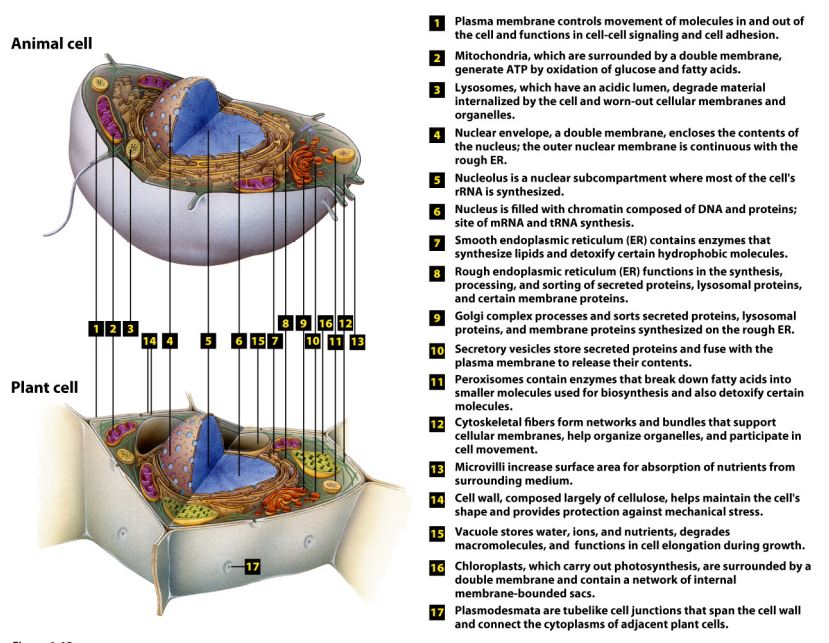
\includegraphics[width=1\textwidth]{images/schemagenerale.JPG}
            \caption{\small cellula animale e vegetale a confronto}
            \label{fig:mesh1}
        \end{figure}

\section{Cellula eucariote}
La struttura interna di una cellula eucariotica risulta più compartimentata e articolata rispetto a quella procariotica. La struttura stessa può variare nello stesso organismo a seconda per esempio del tessuto del quale fa parte. La cellula eucariote è composta da:
\begin{itemize}
    \item membrana plasmatica: controlla il trasporto delle sostanze dall'interno all'esterno e viceversa, si occupa di signaling e adesione
    \item mitocondri: sono organelli circondati da una doppia membrana: quella esterna ha pori grandi e funge da filtro mentre quella interna è più selettiva, lo spazio compreso nella membrana interna si chiama matrice mitocondriale. Generano ATP per ossidazione di glucosio o acidi grassi. Responsabile per la morte cellulare. In una cellula raramente è presente un unico mitocondrio: sono bensì presenti degli agglometari di organelli che comunicano tra loro. Contengono DNA proprio, in particolare un cromosoma circolare (vedi teoria endosimbiontica).
    \item lisosomi: degradano materiale interno alla cellula e materiale cellulare "usurato" o malfunzionante (in quest'ultimo caso si parla di autofagia)
    \item membrana nucleare: doppia membrana che circonda il nucleo, la membrana esterna è in continuità con il RE
    \item nucleo: è un organello dove avviene la sintesi di DNA e mRNA
    \item cromatina: è composta da DNA e proteine
    \item REL: il reticolo endoplasmatico ruvido sintetizza e processa le proteine
    \item RER: il reticolo endoplasmatico liscio contiene enzimi che sintetizzano i lipidie de-tossificano alcune molecole idrofobiche
    \item apparato del Golgi: processa e smista le proteine secrete dal RE e lipidi, è strutturato a cisterne in continuità con il RE
    \item vescicole secretorie: sono vescicole che contengono sostanze che devono essere secrete all'esterno o che viceversa (si fondono con la membrana per permettere il passaggio). Queste operazioni richiedono energia
    \item perossisomi: contengono enzimi che rompono gli acidi grassi
    \item fibre citoscheletriche: consistono nella rete di collegamento intracellulare, sono coinvolte nel movimento della cellula e nel mantenimento della sua struttura. 
    Si dividono in microtubuli (MT), filamenti intermedi (FI) e microfilamenti (MF)
    \item microvilli: aumentano la superficie di assorbimento di nutrienti \\
    \item parete cellulare: nelle cellule vegetali mantiene la forma cellulare e fornisce protezione
    \item vacuolo: nelle cellule vegetali mantiene acqua e nutrienti, degrada macromolecole e serve all'elongazione della cellula durante la crescita
    \item cloroplasti: nelle cellule vegetali compiono il processo di fotosintesi, sono circondati da una doppia membrana, hanno un DNA proprio (vedi teoria endosimbiontica).
    \item plasmodesmata: (?) nelle cellule vegetali, sono giunzioni che connettono il citoplasma di una cellula con quello di altre cellule adiacenti
    \item citoplasma: per esclusione si definisce citoplasma tutto ciò interno alla cellula che non si identifica in un organello.
    
\end{itemize}

       

\section{Organismi modello}

\subsection{Saccharomyces cerevisiae}
Il lievito (\textit{Saccharomyces cerevisiae}) è un organismo eucariote composto di una sola cellula. Proprio per questo motivo è stato ampiamente utilizzato come organismo modello e studiato a fondo. 
Il suo ciclo di vita consiste in una fase aploide e una fase diploide. Un altro motivo per il suo ampio utilizzo è proprio la velocità di duplicazione dovuta alla fase aploide che velocizza l'analisi in ricerca genetica. Risulta inoltre facile da manipolare e poco costoso economicamente. 
Il suo genoma è composto da circa 12.6 milioni di paia di basi (pb). Per dare un confronto, Escherichia coli ne possiede 4.6 milioni e il genoma umano oltre 3.2 miliardi. Possiede sequenze introniche e il meccanismo di espressione dei geni è simile a quella dell'uomo.

\subsection{Chlamydomonas reinhardtii}
L'alga unicellulare \textit{chlamydomonas reinhardtii} è "l'analogo vegetale" per il lievito visto nel paragrafo precedente. Contiene cloroplasti ed effettua la fotosintesi. Anche in questo caso, è un organismo facile da manipolare

\subsection{Caenorhabditis elegans}
Il nematode \textit{Caenorhabditis elegans} è un organismo pluricellulare conosiuto anche come \textit{Roundworm}. Ha fornito la base per molti studi, in particolare per quelli che riguardano la morte cellulare programmata. Da adulto, ha un numero costante di cellule pari a 959

\pagebreak
\setcounter{section}{0}

\large{\addcontentsline{toc}{part}{Capitolo 2: Struttura e funzioni delle proteine}}
\Large\textbf{Capitolo 2: \\ Funzioni e struttura delle proteine}

\section{Struttura gerarchica}
    \small
    L'intero insieme di proteine che può essere espresso dall'organismo prende il nome di \textbf{proteoma}. Il genoma consente di identificare molte più proteine rispetto a quelle effettivamente espresse.
    Le proteine si classificano in 
    \begin{itemize}
        \item dipeptidi: composti da due amminoacidi (AA)
        \item oligopeptidi: composti da meno di 20/30 AA
        \item polipeptidi: composti da 200/500 AA 
    \end{itemize}
    Gli AA di cui si compongono le proteine si dividono nelle seguenti categorie 
    \begin{itemize}
        \item non polari
        \item polari, che a loro volta si dividono in: 
        \begin{itemize}
            \item carichi positivamente
            \item carichi negativamente
            \item neutri
        \end{itemize}
    \end{itemize}
    Gli AA sono legati l'un l'altro tramite legami peptidici, la reazione che porta al legame è una reazione di consensazione (CREDO). La catena amminoacidica si legge a partire dall'AA che espone l'N-terminale fino all'AA che espone il C-terminale (perchè corrisponde all'ordine di sintesi del peptide).\\
    Ogni proteina sintetizzata assume una conformazione tridimensionale dovuti alle interazioni elettrostatiche tra gli AA. L'urea è una molecola che destabilizza la formazione di questi legami. Ci sono enzimi (chaperon) che concorrono alla formazione della conformazione tridimensionale corretta.
    
          \begin{figure}[h]
            \centering
            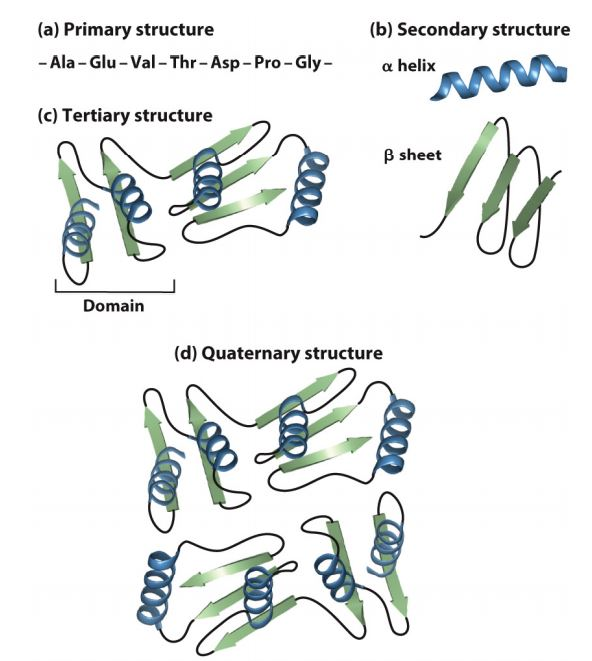
\includegraphics[width=0.5\textwidth]{images/proteinegerarchia.JPG}
            \caption{\small schema generale delle strutture proteiche}
            \label{fig:mesh1}
        \end{figure}
    
    \subsection{Folding}
        \small
        Per \textbf{Folding} si intende il processo di ripiegamento della catena amminoacidica. Questo evento consiste nella formazione di legami (solitamente legami a idrogeno) tra le catene laterali degli AA o il backbone della catena amminoacidica stessa (tutte le combinazioni sono possibili).
        Le ripiegature scorrette possono essere la causa di patologie (per esempio il morbo della mucca pazza).
    
        \subsubsection{Eccezioni}
            In alcuni casi il folding può avvenire tramite interazioni non-covalenti, nonostante ciò si instaurano legami covalenti tra catene polipeptidiche diverse (anche tra le catene laterali dello stesso polipeptide) (?)\\
            
            \textbf{Ponte di-solfuro}  \\
            Il ponte di solfuro si forma su due cisteine, che consolidano interazioni non-covalenti all'interno della cellula cosicché possa mantenere la stessa stabilità all'esterno.
            Esempio: in un anticorpo, le catene pesanti e leggere presentano ponti di-solfuro tra per stabilizzare la molecola.
    
    
    \subsection{Struttura primaria}
        La struttura primaria della proteina consiste nella sequenza amminoacidica di cui è composta, è polarizzata (?) e si considera il primo AA quello che espone l'N-terminale.
    
    
    \subsection{Struttura secondaria}
        La struttura secondaria consiste in ripiegamenti locali della sequenza di AA. Le due strutture secondarie che si riscontrano sono $\alpha -Elica$ ($\alpha E$) e $\beta -Foglietto$ ($\beta F$). 
        
        \subsubsection{$\alpha -Elica$}
            L'$\alpha E$ è un organizzazione 3D che consiste nella disposizione dei residui AA verso l'esterno, è resa stabile per i legami H tra gli atomi del backbone. 
            La sia struttura risulta sempre uguale a se stessa indipendentemente dai residui AA (un ossigeno si lega sempre ad un idrogeno dell'AA quattro posizioni più avanti). Il passo dell'elica corrisponde a 0.54 nm. Per compiere un giro sono necessari 3.6 AA.\\
            Alcuni AA interferiscono con la formazione della struttura, in particolare glicina e prolina.\\
            L'$\alpha E$ può assumere proprietà chimiche differenti a seconda della sequenza AA che la compone. Per esempio può contenere code idrofobiche nel caso l'$\alpha E$ sia destinata a fare parte di un complesso proteico trans-membrana.
            Può essere destrorsa o sinistrorsa.
        
        \subsubsection{$\beta -Foglietto$}
            Il $\beta F$ è basato sulle interazioni H tra gli atomi del backbone. Le catene laterali degli AA sono disposte alternativamente sopra e sotto il piano del foglietto. Anche in questo caso, la sua struttura è indipendente dalla catena AA ed è sempre uguale a se stessa. \\
            Gli \textit{strand} del foglio possono essere orientati in maniera:
            \begin{itemize}
                \item parallela (da un lato del foglietto si trovano tutti gli N-terminali)
                \item antiparallela (l'N-terminale si alterna tra i lati del foglio). 
                Viene chiamato $\beta -turn$ il ripiegamento che connette due filamenti antiparalleli, ha una composizione sistematica di 4 AA.
            \end{itemize}
            Esistono strutture ibride (porzioni parallele e antiparallele).
        
    
    \subsection{Struttura terziaria}
        Per struttura terziaria si intendono ripiegamenti di porzioni più ampie della sequenza AA. 
        
        \subsubsection{Coled-coil motiv}
            La struttura del Coiled-coil si può formare in presenza di due $\alpha E$ che si "arrotolano" su loro stesse. Le eliche che tendono a formare questa struttura comprendono delle sequenze AA specifiche chiamate \textit{heptad repeat} lunghe sette AA. 
            Le posizioni interne a questa sequenza sono spesso indicate con \textit{abcdefg} dove \textit{a} e \textit{d} sono AA idrofobici (1 e 4).
            Le due eliche, avendo caratteristiche simili, tendono ad associarsi per stabilizzarsi. Non si ripiegano necessariamente l'una sull'altra autonomamente.
        
        \subsubsection{Domini}
            Un dominio è una porzione della proteina che comprende più strutture secondarie e assumono una conformazione autonomamente.
        
        \subsubsection{Domini non strutturati}
            Un dominio non strutturato non assume conformazione propria, ma possono interagire con altre molecole per assumere una conformazione specifica. Possono svolgere una funzione di signaling o regolatoria.\\
            
            \textbf{Chaperon}\\
            Il folding di una proteina avviene infatti contemporaneamente alla sintesi, qualora la conformazione 3D attesa debba passare attraverso uno stato energicamente sfavorito, può intervenire uno \textit{Chaperon}, che collabora alla formazione della proteina matura.
        
    
    \subsection{Struttura quaternaria}
        Per struttura quaternaria si intende l'associazione di più polipeptidi per la formazione di un complesso funzionale. 
        Le proteine formate tendono ad assumere conformazioni standard (le conformazioni che effettivamente si riscontrano sono una piccola percentuale rispetto al totale delle combinazioni per un determinato numero di AA).\\
        Le associazioni tra polipeptidi differenti avvengono attraverso legami non-covalenti per la formazione di polimeri. Esistono degli agenti che permettono l'aggregazione di una molecola funzionante (?).
        
     
    
\section{Funzioni}
    Le funzioni delle proteine possono essere talvolta già associate ad una struttura terziaria. In alcuni casi il ruolo di un polipeptide è funzionale ad un complesso strutturalmente più complesso (ad esempio il ribosoma). \\
    Le funzioni principali delle proteine sono:
    \begin{enumerate}
        \item regolatoria
        \item strutturale
        \item movimento della cellula
        \item enzimatica
        \item trasporto
        \item signaling
    \end{enumerate}
    
    
    \pagebreak
\setcounter{section}{0}

\large{\addcontentsline{toc}{part}{Capitolo 3: Struttura della membrana}}
\Large\textbf{Capitolo 3: \\ Struttura della membrana}

\section{Lipidi}
\small
    I lipidi sono una classe di biomolecole che sono caratterizate da una porzione idrofoba. 
    
    \subsection{Acidi grassi}
        Gli acidi grassi sono una categoria di lipidi caratterizzati da una catena idrocarburica più o meno lunga. Qualora compaiano doppi legami tra i carboni della coda, si dice che l'acido grasso è \textit{insaturo}, si dice \textit{saturo} altrimenti. La presenza di code insature favoriscono il comportamento liquido della membrana, al contrario, la presenza di catene insature favoriscono al rigidità.
        
    \subsection{Fosfolipidi}
        I fosfolipidi sono una classe di lipidi composti da due catene idrocarburiche e una testa di glicerolo: la testa è fortemente idrofila mentre la coda fortemente idrofobica.
        Questa struttura conferisce la caratteristica \textit{anfipatica} alla molecola.\\
        La \textit{fosfatidilcolina} è il fosfolipide più abbondante nelle membrane, è composto di colina, fosfato, glicerolo e due code idrofobiche.
        \subsubsection{Fosfogliceridi}
            Sono una categoria di fosfolipidi che si differenziano tra loro in base alla composizione della testa polare, alla quale di aggiunge il di-acil-glicerolo. Tra queste possiamo ricordare \textit{fosfatidil serina}, \textit{fosfatidil inositolo} e \textit{fosfatidil colina}.
            
        \subsubsection{Plasmalogeni}
            Sono una sottoclasse di fosfolipidi caratterizzata da un gruppo vinil-etere in posizione 1 del glicerolo. Le catene idrocarburiche sono legate una tramite un legame etere e una tramite legame estere.
        
    \subsection{Trigliceridi}
        Sono una categoria di lipidi scarsamente anfipatica, proprio per questo motivo non fanno parte della membrana cellulare.
        
    \subsection{Sfingolipidi}
        Sono una categoria di lipidi simili ai fosfolipidi, al posto del glicerolo contengono sfingosina e una testa polare, al quale è legata una catena acida, un gruppo amminico e due gruppi ossidrili. Sono anche esse molecole anfipatiche. ???
        
    \subsection{Steroli}
        Sono una categoria di lipidi presenti negli animali (gli analoghi vegetale sono ergosterolo e stigmasterolo).
        Sono composti da quattro anelli idrocarburici e una coda idrocarburica non polare.\\
        Anche questa categoria presenta caratteristiche anfipatiche dovute alla presenza di un gruppo ossidrile dal lato opposto della catena.\\
        Sono di dimensioni inferiori rispetto ai fosfolipidi, sono presenti nel doppio strato lipidico della membrana: il gruppo OH dello sterolo interagisce con la testa polare dei fosfolipidi e costituiscono una componente più interna.\\
        La funzione di queste molecole all'interno della membrana è legata alla fluidità del mosaico: una maggior concentrazione aumenta la rigidità (nel caso si introducano artificialmente si assiste al comportamento inverso).
        
    \subsection{Glicolipidi}
        I glicolipidi sono una categoria di lipidi che contengono uno zucchero come residuo legato alla testa polare. Sono presenti solo nello strato esterno della membrana. L'aggiunta dello zucchero avviene a livello del Golgi. \\
        La loro funzione comprende l'interazione tra la cellula e l'ambiente, sono punti di ingresso per tossine e sono utili per cariche elettriche e pH. ???
    
\section{Doppio strato lipidico}
    La membrana plasmatica consiste di un doppio strato lipidico, formato prevalentemente da fosfogliceridi, steroli, glicolipidi e sfingolipidi. Tra questi i primi sono i più abbondanti.\\
    La struttura planare di doppio strato lipidico è energicamente sfavorita, se la si pone in soluzione infatti tenderà a richiudersi su se stessa formando un liposoma chiuso (detti micelle qualora non contengano all'interno soluzione acquosa).
    \vspace{0.5cm}
    I vari tipi di lipidi sono presenti in percentuali differenti in porzioni della membrana differenti. Per esempio la sfingomielina è presente al 13\% nelle membrane mieliniche mentre si limita all'8\% nel Golgi e al 3\% nel RE.
    Fosfatidil etanolammina e fosfatidil serina sono invece presenti solo a livello del figlietto citosolico. 
    Al contrario, fosfatidil colina e sfingomielina sono presenti solo a livello del foglietto esoplasmatico.
    Questo suggerisce che i lipidi vengano aggiunti alla membrana e successivamente spostati (a livello di foglietto) da componenti dedicate.
    \subsection{Spostamenti dei lipidi di membrana}
        I lipidi di membrana possono effettuare degli spostamenti di tre tipi:
        \begin{enumerate}
            \item diffusione laterale: si fanno spazio tra i lipidi adiacenti
            \item rotazione sul proprio asse verticale
            \item flip-flop: cambiano il foglietto (da interno a esterno o viceversa).
        \end{enumerate}
        Quest'ultima tipologia di movimento è molto rara se la si considera isolatamente. Tuttavia esistono degli enzimi che catalizzano questo movimento, quali \textit{scramblasi} e \textit{flippasi}.
        \subsubsection{Scambrlasi e flippasi}
            La scramblasi è un enzima lipide-specifico che serve ad ababssare l'energia di attivazione per il flip-flop. \\
            La flippasi è un enzima che idrolizza ATP per promuovere l'asimmetria di lipidi specifici. \\
            Queste due molecole insieme determinano la distribuzione dei lipidi di membrana. Sono coinvolte anche nel caso in cui una cellula debba andare incontro a morte programmata: viene infatti promossa una asimmetria di fosfatidil serina, quindi viene riconosciuta da macrofagi e viene eliminata.
        
    \subsection{Volumi e disposizioni}
        Diverse tipologie di fosfolipidi occupano volumi differenti a seconda della loro composizione. In particolare:
        \begin{itemize}
            \item fosfatidil colina occupa un volume cilindrico
            \item fosfatidil etanolammina occupa un volume assimilabile ad un cilindro, la cui testa occupa il vertice
            \item sfingomielina occupa un volume cilindrico in altezza superiore alla fosfatidil colina
        \end{itemize}
        
        \begin{figure}[h]
            \centering
            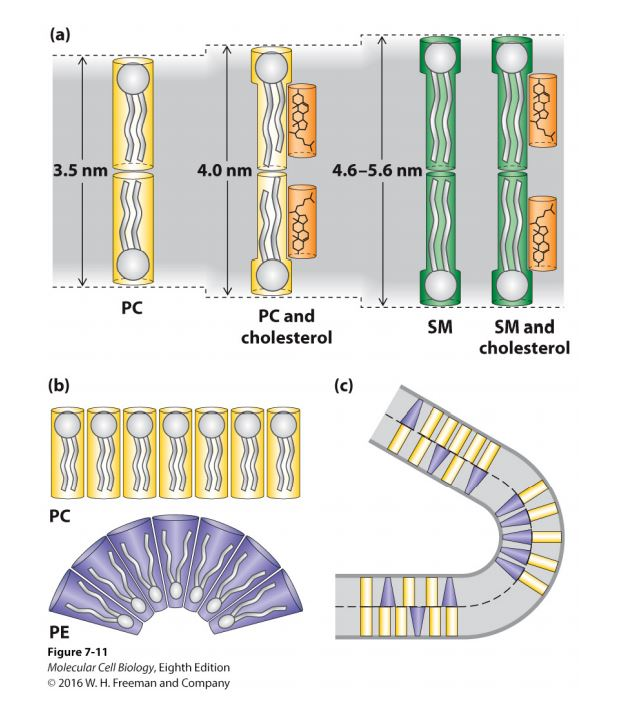
\includegraphics[width=0.5\textwidth]{images/doppiostrato.JPG}
            \caption{\small volume della membrana in relazione a lipidi differenti}
            \label{fig:mesh1}
        \end{figure}
        
        In base alle componenti dei foglietti lipidici, la membrana assume conformazione e spessore differente:
        \begin{itemize}
            \item un doppio strato di fosfatidil serina combinato con degli steroli aumenta lo spessore rispetto a un doppio strato di fosfatidil serina semplice
            \item un doppio strato di sfingomielina combinato con degli steroli \textit{non} aumenta lo spessore rispetto a un doppio strato di sfingomielina semplice. Essendo la sfingomielina \textit{un cilindro più alto}, questo doppio strati risulta più spesso di quello di fosfatidil serina.
            \item la presenza di fosfatidil etanolammina induce un ripiegamento.
        \end{itemize}

        Esistono processi che permettono una temporanea formazione di zattere lipidiche (composizione specifica locale di lipidi) per specializzazioni della membrana.\\
    
\section{Proteine di membrana}
    \small
    Ogni membrana incorpora delle proteine con funzionalità specifiche.
    \subsection{Tipologie di proteine di membrana}
        Le proteine di membrana possono essere integrali, ancorate a lipidi o periferiche di membrana. Molto raramente si può trattare di un $\alpha E$ associata ad un mono-strato.
        
         \begin{figure}[h]
            \centering
            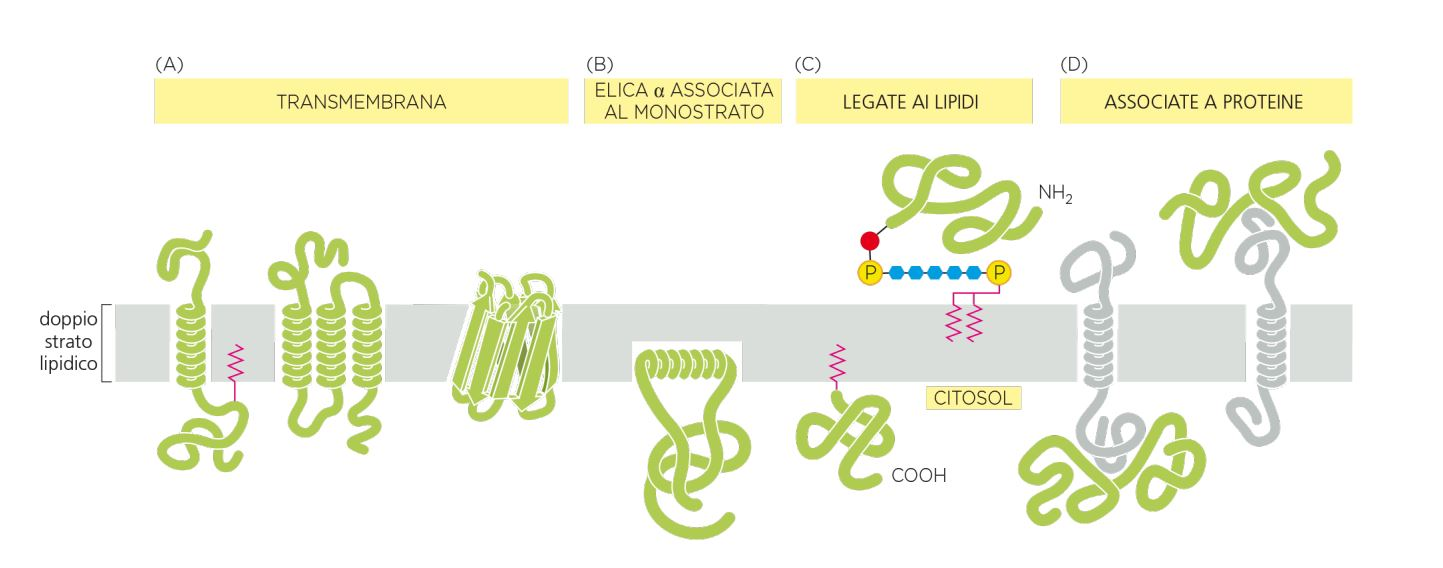
\includegraphics[width=1\textwidth]{images/proteinemembrana.JPG}
            \caption{\small tipologie di proteine di membrana}
            \label{fig:mesh1}
        \end{figure}
        
        \subsubsection{Integrali di membrana}
            Consistono di tre domini:
            \begin{enumerate}
                \item transmembrana: la porzione che effettivamente attraversa il doppio strato lipidico.
                \item luminale o extracellulare: il dominio che volge sul lumen o all'esterno della cellula
                \item citosolico: la parte che si interfaccia con il citosol
            \end{enumerate}
            Attraversano da parte a parte la membrana una (\textit{single pass}) o più volte (\textit{multi pass}) la membrana cellulare. Un passaggio è composto di un elica di circa 20/25 AA (a seconda della composizione della membrana attraversa spessori differenti).\\
            Una proteina single-pass termina solitamente con le cariche negative volte verso il lumen o porzione extracellulare e la porzione positiva verso il citosol.\\
            Di seguito degli esempi di proteine transmembrana costituite di $\alpha E$:
            \begin{itemize}
                \item {Glicoforina a dimero}:
                La struttura di questa proteina presa singolarmente attraversa la membrana tramite una sola $\alpha E$, la sua struttura quaternaria è composta di due di queste molecole.
                L'associazione di due proteine è promossa dall'interazione delle due $\alpha -E$ per formare un coiled-coil transmembrana.
                \item{Acuaporina}:
                L'acquaporina è un esempio di proteina multipass: la struttura terziaria è composta di sei $\alpha E$ transmembrana diagonali ad essa, quella quaternaria comprende quattro di questi domini e permette la formazione di canali acquosi.
                \item{Rodopsina}:
                La rodopsina è un esempio di proteina multipass composta di sette $\alpha E$ transmembrana perpendicolari ad essa.
                \item{TRC (\textit{T-cell-receptor})}:
                è una struttura che consiste di complessi carichi che si associano perchè energicamente favoriti.
            \end{itemize}
            Un canale transmembrana costituito di $F\beta$ sono le porine: sono strutturate a $\beta barile$, le componenti transmembrana sono idrofiliche verso l'interno e idrofobiche verso l'esterno. Generalmente le proteine di membrana con $F\beta$ sono più rigide.
            
        \subsubsection{Ancorate a lipidi}
            Le proteine ancorate ai lipidi non possiedono una porzione proteica ancorata al doppio strato, bensì sono solamente affacciati sul citosol o sulla porzione extracellulare.
            Sono tipicamente globulari, possiedono una componente idrofilica e sono covalentemente legate ai lipidi tramite una delle seguenti reazioni:
            \begin{itemize}
                \item alcilazione
                \item prenilazione
                \item GPI anchor (\textit{glicosil fosfatidil inositolo}, un glicolipide, componente saccaridica si lega alla proteina), tipicamente extracellulari
            \end{itemize}
            
        \subsubsection{Periferiche di membrana}
            Sono associate temporaneamente alla membrana tramite legami non covalenti, per esempio possono associarsi ad altre proteine transmembrana. Esistono diverse fosfolipasi che idrolizzano legami differenti. Sono usate sperimentalmente su cellule intatte per verificare la composizione del foglio esterno della membrana. Enzimi idrofili?
        
        \subsubsection{Proteine e lipidi glicosilati}
            A livello della membrana sono comprese anche proteine e lipidi associati alla membrana glicosilati. \\
            Nelle cellule eucariotiche il \textit{cortex} è costituito in larga parte di \textit{spettrina} che forma reticolo sulla faccia citoplasmatica che si associa ad altre proteine transmembrana e ne conferisce determinate proprietà meccaniche.\\
            Ad esempio i gruppi sanguigni umani sono oligosaccaridi ancorati sul lato extracellulare della membrana. Hanno una configurazione di base alla quale possono aggiungersi precisi monosaccaridi per determinare i gruppi A o B. 
            
    \subsection{Detergenti}
        Al fine di studiare le componenti proteiche facenti parte della membrana cellulare, è possibile utilizzare un detergente per estrarle tramite solubilizzazione con un \textit{detergente}.\\
        I detergenti sono sostanze anfipatiche che stabilizzano la porzione idrofoba della proteina. Possono essere ionici o non-ionici.
        \subsubsection{Ionici}
            Sono detergenti "aggressivi", talvolta sono troppo efficaci al fine dell'estrazione della proteina e possono portare alla denaturazione della proteina. Formano una micella attorno alla proteina. Un esempio è \textit{SDS}, che ha carica netta e viene associato ad uno ione.
        \subsubsection{Non-ionici}
            Sono detergenti con una polarità ma non una carica netta, questo permette di evitare la denaturazione della proteine, dissolvendo le proteine ma non formando micelle nette. 
            Sopra una certa concentrazione del detergente anche in questo caso di va incontro alla formazione di una micella: si parla ci \textit{CMC}, ovvero \textit{critical mycell concentration}.
        
    \subsection{Studio delle proteine di membrana}
        \subsubsection{FRAP}
            FRAP (\textit{fluorecence recovery after photoblieaching}) è una tecnica che si può usare sperimentalmente per verificare la migrazione dei lipidi sulla membrana. \\
            Il processo consiste nel marcare una determinata zona della membrana cellulare con fluorescenza. Applico un bleaching in un dominio di membrana limitato ("spegnendo" la fluorescenza localmente) e osservo nel tempo la ricomparsa della fluorescenza in quella zona.\\
            La ricomparsa della fluorescenza in rapporto al tempo indica la capacità di migrazione dei lipidi attraverso la membrana, ovvero il \textit{coefficente di diffusione}.
        \subsubsection{SPT o SMT}
            SPT o SMT (\textit{single particle/molecule tracking}) è una tecnica per visualizzare il movimento di una singola molecola nel tempo.\\
            Analizzandone il tracciato si può dedurre se una molecola è libera o ha una bassa motilità.
        
\pagebreak
\setcounter{section}{0}

\large{\addcontentsline{toc}{part}{Capitolo 4: DNA e cromosomi}}
\Huge\textbf{Capitolo 4: \\DNA e cromosomi}
\small
\section{Storia, scoperte ed esperimenti}
    L'informazione genetica di una cellula è contenuta all'interno dei cromosomi. Questi sono fatti di acidi nucleici e proteine. Inizialmente si pensava che le proteine fossero la base dell'informazione genetica perchè si associava la variabilità degli AA a una maggiore variabilità genetica.
    \subsection{Fredrick Griffith}
        Nel 1928, Griffith esegue un esperimento che certifica la trasformazione batterica. Prende due ceppi di Streptococcus pneumonae:
        \begin{itemize}
            \item ceppo S (smooth, presenta glicocalice), patogeno per l'organismo topo
            \item ceppo R (rough), innocui per il topo
        \end{itemize}
        Si effettuano i seguenti esperimenti:
        \begin{enumerate}
            \item inoculo del ceppo S nel topo, il topo muore. Facendo una biopsia post mortem si riesce a risontrare lo stesso ceppo nell'organismo.
            \item inoculo del ceppo R nel topo, il topo non ne risente.
            \item inoculo del ceppo S inattivato al calore nel topo, il topo non ne risente.
            \item inoculo del ceppo S inattivato al calore insieme al ceppo R nel topo, il topo sviluppa la malattia e muore. Facendo una biopsia si riscontra il ceppo S.
        \end{enumerate}
        Si deduce che avviene una cerca comunicazione tra i batteri per lo scambio di informazioni, si parla quindi di \textit{trasformazione batterica}.
        
    \subsection{Avery, MacLeod e McCarty}
        Nel 1944, questi scienziati condussero esperimenti sul ceppo patogeno S di cui si è parlato nell'esperimento precedente. In particolare il ceppo S viene esposto a tre enzimi:
        \begin{enumerate}
            \item DNAasi
            \item RNAasi
            \item Proteasi
        \end{enumerate}
        Si osserva che solo nel primo caso il ceppo non è più in grado di eseguire la trasformazione batterica di cui si parlava nell'esperimento precedente. Di conseguenza il DNA degradato era responsabile per il mancato trasferimento dell'informazione genetica.
    
    \subsection{Hershey e Chase}
        Nel 1952, Hershey e Chase usarono un batteriofago T2 contro E. Coli. Si era a conoscenza che il fago contenesse le informazione genetiche per produrre copie di se stesso e si sapeva che il virus fosse composto solo di DNA e proteine.
        \begin{enumerate}
            \item Si marcarono le proteine con l'isotopo S35 e il DNA con P32. 
            \item E. Coli ospita i fagi e ne avviene la replicazione
            \item Il tutto viene centrifugato per ottenere l'isolamento delle molecole pesanti.
        \end{enumerate}
        Il battere infettato contiene P32, di conseguenza è il DNA a veicolare l'informazione genetica.
    
    \subsection{Watson, Crick e Franklin}
        Nel 1953, questi tre scienziati cercarono di comprendere la struttura tridimensionale della molecola del DNA. Si scoprì che è composta dalle quattro basi azotate legate tra loro attraverso un numero differente di legami H (tre per la coppia CG e due per AT). 
        La conformazione tridimensionale prescinde dalle basi azotate presenti all'interno. A e G sono purine (due anelli) mentre C e T sono pirimidine (singolo anello).\\
        Grazie alla cristallografia a raggi X, si dedusse la conformazione a doppia elica del DNA associate in maniera antiparallela.\\
        Si giunse alla conclusione che ogni cellula racchiudeva il meccanismo per la sua duplicazione, trasferendo alla cellula figlia la stessa informazione genetica.
    
\section{Struttura}
    \small
    La cellula eucariotica è diploide (ad esclusione dei gameti), quelle umane comprendono circa 3.2 miliadri di pb, divisi in 22 coppie di cromosomi più una sessuale. Il cariotipo è l'insieme di tutti i cromosomi.\\
    I geni sono le sequenze del DNA deputate alla produzione di proteine, ovvero geni. Nell'uomo le sequenze codificanti sono meno dell'1\%. 
    Il resto è composto da DNA intergenico che ha tuttora funzioni ignote (DNA \textit{spazzatura}, probabilmente non sono inutili ma hanno una funzione non ancora intuita), tuttavia certamente non codificanti.\\
    Un gene è codificato da uno dei due filamenti, il filamento complementare solitamente non è codificante.\\
    Per traslocazione si intende lo spostamento di specifiche porzioni del genoma in porzioni differenti del DNA, causando possibilmente un fenotipo patologico. Questo tipo di eventi avviene spesso nelle cellule tumorali.\\
    C'è correlazione tra il numero di geni e la complessità dell'organismo ma non tra la lunghezza effettiva del genoma (o numero di cromosomi) e complessità dell'organismo.
    
    \subsection{Fasi del ciclo cellulare}
        Le fasi del ciclo di vita della cellula si possono dividere in:
        \begin{itemize}
            \item Interfase in cui è presente il nucleo ben definito. Abbiamo espressione genica e la replicazione dei cromosomi è attiva. 
            L'interfase è composta da fase G0 (fase di vita cellulare esonerata dal ciclo replicativo), G1 (periodo durante il quale si costituiscono nuovi componenti per fare fronte alle fasi successive), S (\textit{sintesi}, viene sintetizzato nuovo DNA) e G2 (nuovo periodo in cui accrescono le quantità di molecole necessarie).\\
            \item Fase M, ovvero la mitosi (divisa in profase, prometafase, metafase, anafase e telofase). Durante la mitosi avviene la compattazione del materiale genetico in cromosomi e la segregazione ai poli.
        \end{itemize}
    
     \begin{figure}[h]
            \centering
            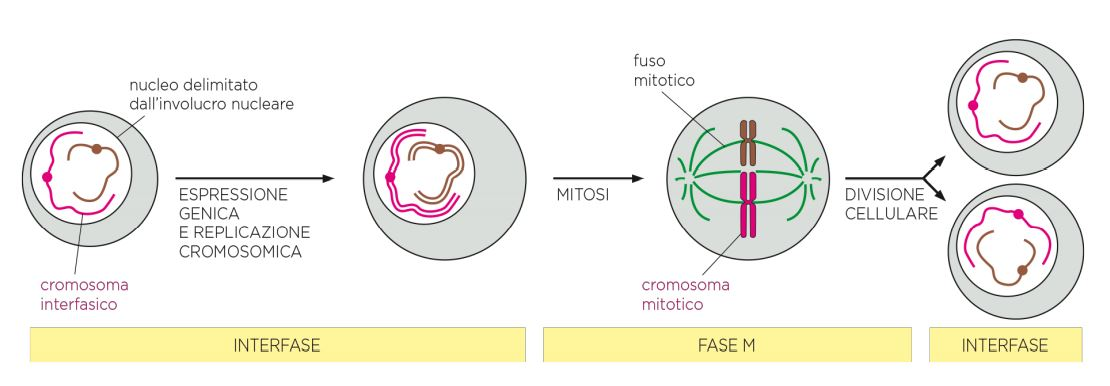
\includegraphics[width=1\textwidth]{images/mitosiBreve.JPG}
            \caption{\small fasi del ciclo cellulare in breve}
            \label{fig:mesh1}
        \end{figure}
    
    \subsection{Cromosomi eucariotici}
        I cromosomi (dopo la fase S) sono composti da due cromatidi fratelli, una zona centromerica, molteplici origini di replicazione (ORI) e telomeri alle estremità.\\
        Durante la fase S, ORI viene localmente "aperto" e si procede alla sintesi di un nuovo filamento sullo stampo dei due disponibili. I due cromatidi sono tenuti assieme dal cinetocore (nella zona centrometica) che consente interazioni con elementi citoschelettrici.
        I telomeri sono sequenze nucleotidiche ripetute alle estremità del filamento che consentono la replicazione di queste.\\
        Durante la fase I, il DNA è molto più svolto all'interno del nucleo formando la cromatina. Si nota comunque che cromosomi diversi sono confinati in aree specifiche della cromatina.\\
        Il DNA può assumere due gradi di avvolgimento:
        \begin{itemize}
            \item regioni eterocromatiche, zone che contengono geni non esprimibili a causa dell'elevata compattezza
            \item regioni eucromatiche, sono la maggioranza e possono contenere geni esprimibili.
        \end{itemize}
        Il cromosoma svolto è 10.000 volte più lungo del cromosoma mitotico (cinque ordini di grandezza).
        
        \subsubsection{Riavvolgimenti e compattazione}
            Per \textit{nucleosoma} si intende il DNA avvolto su dischi proteici, composti da proteine \textit{istoniche}, per la formazione di una struttura a \textit{collana di perle}. Attorno al disco si arrotolano 1.7 giri di DNA (147 basi per formare un nucleosoma). 
            Tra una proteina e l'altra di identifica il DNA di connessione. Questa struttura può essere disassemblata da enzimi che conducono attività nucleasica.\\
            
            \textbf{Istoni}\\
                Il disco proteico è composto da otto istoni (subunità), in particolare di quattro polipeptidi, ognuno presente in due copie: H2A, H2B, H3 e H4.\\
                Gli istoni sono molto basici (per associarsi al DNA carico negativamente), l'N-terminale protrude all'esterno del disco per ogni istone. Sono proteine estremamente conservate tra speci diverse. Il DNA avvolto attorno ai dischi risulta 3 volte più corto.\\
                L'istone H1 non fa parte del core dell'ottamero, ma si associa a nucleosomi differenti e trasforma la struttura in fibra cromatinica. Non è ancora conosciuto il procedimento attraverso il quale il DNA si ripieghi formando anse.
                Nel caso della porzione di DNA su cui si andrà a formare il cinetocore si ha una differenza locale nella struttura istonica (CEMP-A al posto di H3, dalla quale dipende la formazione delle altre proteine del cinetocore).
                
            \begin{figure}[h]
                \centering
                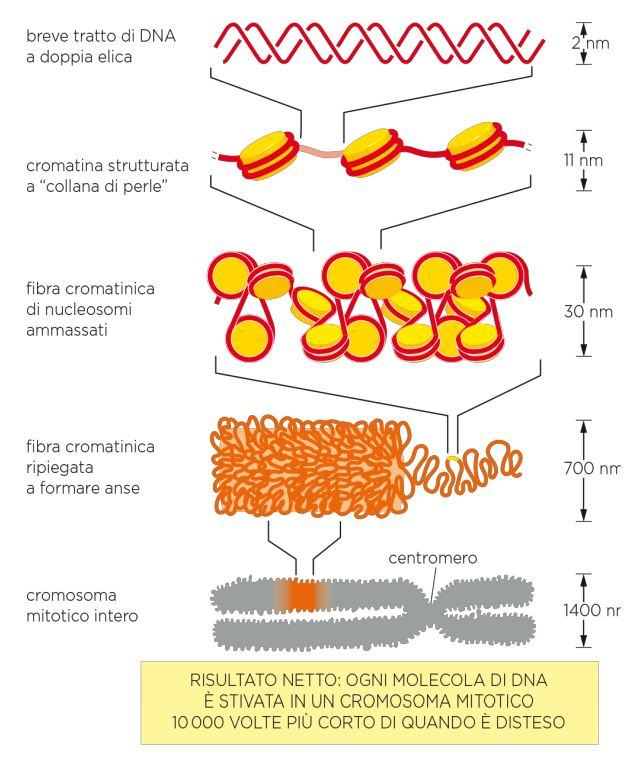
\includegraphics[width=0.75\textwidth]{images/compattazioneDNA.JPG}
                \caption{\small schema degli stadi della compattazione del DNA in cromosomi}
                \label{fig:mesh1}
            \end{figure}
        
        \subsubsection{Svolgimenti e decompattazione}
            Lo svolgimento del materiale genetico richiede energia ed è dunque sfavorito. Sono quindi necessari dei complessi per la decondensazione della cromatina. Ogni N-terminale degli istoni può subire delle modifiche chimiche post traduzionali (metilazione, fosforilazione, acetilazione) in maniera specifica che fungono da segnale: determinano la struttura 3D e hanno significati diversi, ad esempio possono indicare lo spegnimento del gene o il suo aumento di espressione.\\
            L'accessibilità della sequenza nucleotidica ne determina l'espressione:
            \begin{enumerate}
                \item eucromatina: è la porzione più abbondante e rappresenta contenuto accessibile ed esprimibile
                \item eterocromatina: è una porzione non accessibile e non esprimibile perchè molto compatta, ne fanno parte telomeri e centromero.
                \item porzioni intermedie tra eterocromatina e eucromatina
            \end{enumerate}
            L'accessibilità à determinata dalle modifiche istoniche della cromatina: una modifica dell'istone può propagarsi "automaticamente" fino a una determinata sequenza isolante che funge da barriera.\\
            Nel caso di un individuo di sesso femminile, vengono utilizzate le informazioni presenti solamente su uno dei due cromosomi sessuali, per questo uno dei due viene "spento" effettuando per l'appunto modifiche post traduzionali dell'istone (diventa interamente eterocromatico). In alcuni casi (come quello del gatto calico) vengono silenziate zone solo localmente. Questo avviene in fasi precoci dell'embriogenesi.
        
\section{Duplicazione}
    Ogni filamento di DNA viene usato come stampo per la sintesi di una nuova molecola di DNA completa. Il processo avviene in maniera semiconservativa. I legami H tra le basi azotate conferiscono grande stabilità alla molecola, per denaturare la struttura occorre aumentare la temperatura superando i 95° C. 
    La duplicazione del genoma umano (3.2 miliardi di basi) avviene in meno di 8 ore.\\
    La temperatura di melting tuttavia dipende dalla percentuale di basi azotate (oltre alla sua lunghezza) presenti sul filamento: infatti se sono presenti più G o C, la temperatura di denaturazione sarà più alta perché sono legate attraverso tre interazioni H al posto di due (quelle tra A e T). 
    In particolare si assume una regola spannometrica per cui per ogni C o G si aumenta la temperatura di 4°C e per ogni A e T si aumenta di 2°C.\\
    Tuttavia nella fase di replicazione, il DNA deve essere localmente denaturato per consentire l'appaiamento delle basi, in questo caso la temperatura sarà stabile a 37°C e la denaturazione non sarà mediata dalla temperatura.
    L'inizio della denaturazione del DNA per la replicazione avviene in una zona che comprende A e T per facilitare il processo.\\
    L'origine della replicazione nel genoma batterico è identificata da un'unica ORI (il cromosoma è circolare, in più non sono presenti istoni).
    Per le cellule eucariotiche, e in particolare quelle umane, esistono più di 10.000 ORI differenti, più di una per ogni cromosoma (circa 220 per cromosoma, ovviamente dipende dalla dimensione del cromosoma). Quindi in fase di replicazione convivono più bolle replicative.
    
    \subsection{Teorie di replicazione}
        Le teorie sulla replicazione del DNA si dividevano in tre categorie:
        \begin{enumerate}
            \item conservativa: il nuovo filamento di DNA sintetizzato non eredita fisicamente nessuna porzione del DNA padre ma è tutto prodotto ex novo.
            \item semi-conservativa: un filamento di ogni molecola di DNA deriva dal padre.
            \item dispersiva: ogni filamento del padre è segmentato e ricucito tra due figli, ogni filamento contiene delle porzioni randomiche derivanti dal padre.
        \end{enumerate}
        \subsubsection{Meselson e Stahl}
            Nel 1958, questi due scienziati provarono la semiconservatività del processo di duplicazione del DNA. In particolare prepararono due colture batteriche marcate rispettivamente con isotopi di N15 e N14. La densità del primo risulterà maggiore di quella del secondo.\\
            Queste due colture vengono messe in contatto e si lasciato incubare nuovamente. Successivamente, centrifugando il campione ottenuto (centrifugazione a gradiente) si osserva che i batteri formavano uno strato omogeneo: questo condusse ad un esclusione della teoria conservativa perché se quello fosse stato il caso sarebbero state visibili due bande distinte.\\
            Sottoponendo poi il DNA delle colture ad una denaturazione, si è potuto notare che si venivano a formare due fasce ben definite, prova del fatto che la duplicazione del DNA avviene in maniera semi-conservativa (se così non fosse stato, si sarebbe riscontrata una fascia uniforme).
        
        \subsection{Neosintesi}
            Il processo di neosintesi comincia con la formazione di una forcella replicativa (locale denaturazione del DNA) e la sintesi avviene su entrambi i filamenti esposti, quindi bidirezionale. \\
            L'enzima che catalizza la sintesi è la DNA Polimerasi (DNA-P) che aggiunge nuovi nucleotidi in direzione 5' - 3'. La sintesi quindi avviene solo sull'estremità 3'.\\
            Il filamento stampo determina la sequenza nucleotidica, le basi vengono legate tra loro tramite un legame fosfodiesterico, rilasciando una molecola di acqua (condensazione).
            La DNA-P lavora in maniera processiva, ovvero inserisce continuativamente i nucleotidi senza dissociarsi. Non tutte le forcelle operano in modo sincrono. \\
            Muovendosi, la forcella replicativa denatura i filamenti di cui uno risulta leggibile da 5' - 3' mentre uno da 3' - 5'. 
            \subsubsection{Leading strand}
                Il filamento che viene letto in direzione 5' - 3' è detto \textit{leading strand} e la sua sintesi avviene in modo continuativo ad opera della DNA-P.
            
            \subsubsection{Lagging strand}
                Il filamento disponibile in direzione 3' - 5' non può essere sintetizzato in maniera diretta dalla DNA-P perchè essa può procedere solo aggiungendo nucleotidi all'estremità 3'. Per questo la DNA-P sintetizza nuovo DNA in frammenti 5' - 3' (Okazaki fragments) che verranno poi "ricuciti" successivamente.
            
            \begin{figure}[h]
                \centering
                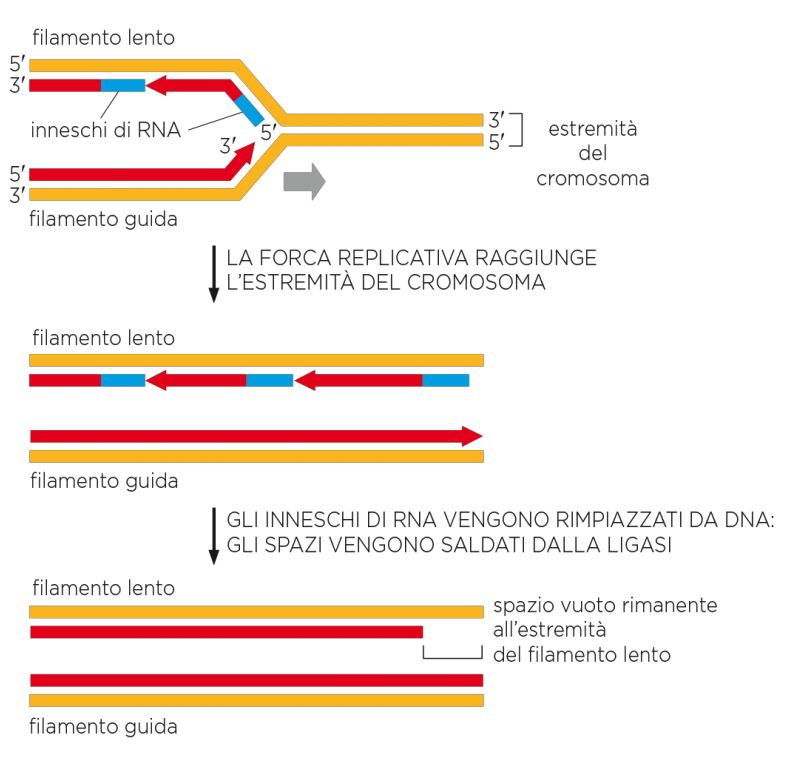
\includegraphics[width=0.75\textwidth]{images/forcellareplicativa.JPG}
                \caption{\small forcella replicativa, frammenti di Okazaki, leading strand e lagging stand}
                \label{fig:mesh1}
            \end{figure}
        
        \subsection{DNA-polimerasi}
            La DNA-P è formata da due domini funzionali:
            \begin{itemize}
                \item un dominio P: consiste nel sito catalitico per la polimerizzazione
                \item un dominio E: che funge da sito catalitico per l'autocorrezione (proof reading, vedi in seguito)
            \end{itemize}
            La direzione per la polimerizzazione è unica (verso 3') e per sintetizzare il resto del filamento occorre partire da uno già esistente ossia una sequenza \textit{primer}.  \\
            Un primer è uno stratch nucleotidico complementare ad un altro acido nucleico che è necessario per iniziare l'attività di DNA-P. Nel contesto umano, il primer consiste in un frammento di RNA di circa 10 pb sintetizzato dalla primasi.\\
            Per il lagging strand ci sono delle sequenze primer per ogni frammento di Okazaki. Nel momento in cui DNA-P raggiunge un primer dopo aver sintetizzato il frammento, interviene una nucleasi che degrada il primer e una specifica DNA-P (*) prosegue utilizzando le basi con desossiribosio corrette: questa è meno processiva di DNA-P menzionata fino ad ora per limitare i danni.
            Successivamente interviene la DNA ligasi che forma il legame tra i due frammenti di Okazaki consumando ATP.
                
        \subsection{Step della sintesi}
            \begin{enumerate}
                \item \textbf{attività dell'elicasi}\\
                L'elicasi idrolizza ATP per catalizzare la denaturazione del filamento. La DNA-P lavora subito dopo la denaturazione così da evitare che le basi si riassocino (per il leading strand). Il lagging strand invece rimane singolo finchè non interviene la primasi.\\
                Esistono delle \textit{single strand DNA binding proteins} che evitano che il filamento di DNA si ripieghi su se stesso.
                \item \textbf{clamp}\\
                La DNA-P si associa al filamento e viene mantenuta stabile da un trimero chiamato \textit{sliding clamp}, negli eucarioti \textit{PCNA} ovvero \textit{Proliferating cell nuclear antigen}. Di questa proteina è stata studiata la distribuzione per capire se la cellula sta replicando il DNA.
                \item \textbf{topoisomerasi}\\
                Vi è la formazione di una tensione sul DNA non denaturato che viene risolta dalla topoisomerasi che opera dei piccoli "tagli" su un filamento in modo da eliminare i superavvolgimenti (e successivamente interviene la ligasi per riallacciare la sequenza).
                \item \textbf{telomeri}\\
                Non è possibile secondo questo procedimento effettuare la sintesi dell'inizio della sequenza del lagging strand in 5'. Per evitare l'accorciamento del DNA a scapito di sequenze utili, sono presenti le sequenze telomeriche all'estremità. Sono delle porzioni di DNA con delle caratteristiche specifiche:
                \begin{itemize}
                    \item sono delle sequenze che proteggono il cromosoma generando un segnale che invoca l'intervento di cromatina (eterocromatica) dedicata per la protezione delle estremità (un'estremità libera per la cellula genera segnali di stress)
                    \item forniscono meccanismo per la sintesi delle estremità tramite una ribonucleoproteina dedicata. Questa aggiunge sequenze su un filamento stampo consentendo l'appaiamento della fine del DNA, le sequenze sono complementari a quella che viene portata dalla telomerasi. 
                \end{itemize}
            \end{enumerate}
            \begin{figure}[h]
                \centering
                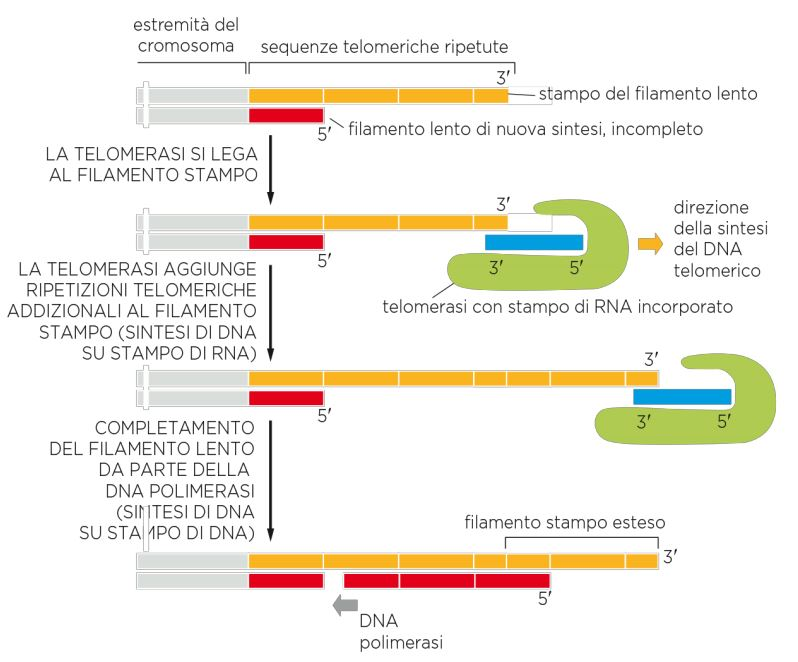
\includegraphics[width=0.75\textwidth]{images/telomero.JPG}
                \caption{\small funzionamento della sequenza telomerica}
                \label{fig:mesh1}
            \end{figure}
            
            \subsubsection{Telomeri e senescenza}
                Nelle celllule somatiche gli enzimi per la telomerasi non sono espressi e la sequenza telomerica si accorcia ad ogni ciclo di replicazione. 
                Al contrario nelle cellule uovo e negli spermatozoi al sequenza telomerica raggiunge la sua lunghezza massima.\\
                Per senescenza si intende il processo degradativo della cellula a causa della perdita dei porzioni telomeriche.\\
                
                \textbf{Esperimento di Hayflick}\\
                Nel 1962, Hayflick condusse un esperimento su cellule epiteliali. Se ne favorisce la proliferazione e si nota che questo processo non viene sostenuto per una quantità temporale indeterminata:
                si evidenzia una fase di crisi dopo circa 50 duplicazioni per poi fare fronte al decadimento effettivo della coltura. Le cellule restano in vita ma non proliferano.\\
                Nelle cellule di un neonato questo processo avviene dopo a confronto di cellule di un anziano. Si associa alla senescenza l'esaurimento delle sequenze telomeriche.\\
                Le cellule tumorali esprimono la telomerasi, quindi non vanno incontro a senescenza: per questo motivo si duplicano per tempi indetermianti.
                
\section{Mutazioni ed errori}
    Le mutazioni a livello di sequenza nucleotidica possono causare gravi patologie o essere incompatibili con la vita.
    Il tasso di errore della DNA-P è molto basso (1 su 10.000.000) perchè gli appaiamenti corretti sono favoriti energicamente. Tuttavia il $\Delta$ energetico non è tale da giustificare un tasso di errore così basso.\\
    L'appaiamento corretto delle basi è dovuto a altri fattori, ovvero: 
    \begin{itemize}
        \item la catalisi di introduzione di un nuovo nucleotide è selettiva per l'appaiamento corretto (forza il nucleotide corretto)
        \item nel caso la polimerasi eucariotica compia un errore svolge un \textit{attività di correzione di bozze} (proof reading), ovvero un'attività che coesiste all'elongazione ma controlla l'appaiamento corretto. \\
        Nel caso la polimerasi sbagli, viene riconosciuto l'errore, torna indietro idrolizzando il legame, rimuovendo il nucleotide sbagliato e inserendo quello corretto. \\
    \end{itemize}
    Risulta necessario per l'attività di proof reading di essere direzionata, infatti rimuovendo l'ultimo nucleotide aggiunto risulta disponibile l'elongazione al 3', se così non fosse ci sarebbe l'estremità al 5' libera che la DNA-P non potrebbe elongare per la sua natura.\\
    
    \subsection{Mutazioni tramite processi spontanei}
        \subsubsection{Depurinazione}
            Per depurinazione si intende la perdita di una purina per idrolisi. Avviene perchè la DNA-P perde una base nel processo di sintesi.
        \subsubsection{Deamminazione della citosina}
            La citosina perde un gruppo amminico e diventa uracile. Nelle replicazioni successive verrà inserita una adenina al posto di una guanina.
    
    \subsection{Mutazioni tramite altri processi}
        \subsubsection{Dimeri di timina}
            La formazione di dimeri di timina non è un processo spontaneo ma aumenta all'aumentare delle radiazioni (UV). Si effettua un legame chimico tra due timine sullo stesso filamento, quando la DNA-P cerca di sintetizazre il filamento non riesce ad interpretare la base da associare.
        \subsection{Radiazioni ionizzanti}
            Vengono introdotti ioni nella struttura chimica del DNA rompendo la struttura stessa.
            I telomeri vengono protetti da cappucci proteici.
            Le terminazioni del DNA possono essere ricucite da una ligasi secondo due alternative:
            \begin{itemize}
                \item \textbf{non omologus ends join}: la ligasi salda qualunque estremità piatta, senza cappucci proteici o telomeri. Questo tipo di saldatura è prona ad errori e può succedere un inserimento o una delezione di una base.
                \item \textbf{omologus ends join}: avviene solamente qualora il DNA sia già stato replicato (G2) e il duplex danneggiato è prossimo a quello omologo. La cellula cerca la sequenza non danneggiata per aggiustare il filamento danneggiato.
            \end{itemize} 
            Per esempio l'anemia falciforme è dovuta alla mutazione di un unico nucleotide, la stessa mutazione ha riscontrato una certa importanza nella difesa della malaria (nelle zone del mondo in cui la malaria è più diffusa è anche più diffuso questo tipo di anemia).\\
            Nel caso di una mutazione dei geni coinvolti nella riparazione degli errori, abbiamo un acucmulo di mutazioni a cascata.
        
     \subsection{Metodi di riparazione}
        \subsubsection{Nucleotide excision repair}
            Viene scisso il nucleotide sbagliato e viene sostituito da DNA-P(*), successivamente interviene la ligasi.
        \subsubsection{Mismatch repair}
            Viene tolta la base sabagliata e viene corretta, non è scontato sapere quale delle due basi sui due filamenti sia quella corretta.

\pagebreak
\setcounter{section}{0}

\large{\addcontentsline{toc}{part}{Capitolo 5: Dal DNA alle proteine}}
\Huge\textbf{Capitolo 5: \\Dal DNA alle proteine}

\vspace{1cm}
\small
I geni sono sequenze di DNA che danno origine a proteine, non tutti i geni sono espressi allo stesso modo (solamente quelli codificanti), infatti esistono dei sistemi che ne regolano l'espressione. 
Non tutti i geni sono contemporaneamente espressi, un gene può essere trascritto molteplici volte.\\
L'RNA differisce dal DNA per alcune caratteristiche:
\begin{itemize}
    \item lo zucchero che lo compone è ribosio invece che desossiribosio (è presente un gruppo OH in 2' invece che un H)
    \item viene utilizzata la base uracile al posto della timina (U ha un gruppo H in posizione 5' mentre T ha un CH$_ {3}$), l'appaiamento con A è identico
    \item l'RNA solitamente consiste di un singolo filamento e ha molte forme eterogenee a livello strutturale. 
\end{itemize}

\section{Trascrizione}
    Il processo di trascrizione, ovvero la trascrizione dello stretch di DNA in uno di RNA, avviene grazie ad un melting locale della doppia elica di DNA, l'appaiamento delle basi con la temporanea formazione di un eteroduplex sfruttando l'appaiamento di nucleotidi. 
    Il tutto è mediato dalla RNA polimerasi (RNA-P) che lavora inserendo nucleotidi in 3' in maniera processiva. Solo un filamento di DNA viene utilizzato come filamento stampo.\\
    L'RNA è solitamente composto da poche kb. La formazione dell'eteroduplex trasla con l'avanzamento della RNA-P, non è necessaria la presenza di un primer, non corregge errori (non è grave come per la duplicazione del DNA in quanto si limita alla produzione di un singolo RNA e una singola proteina). 
    Il tasso di errore della RNA-P è di 1 su 10000 (tre ordini di grandezza più frequenti rispetto alla DNA-P).\\
    La sintesi avviene grazie all'idrolisi di ATP (analogamente a quando avviene per la sintesi del DNA).\\
    Solitamente avviene la trascrizione di più molecole di RNA contemporaneamente (ad opera di più RNA-P) da un singolo stretch di DNA. La RNA-P ha una velocità di circa 1.5 kb ogni 50 secondi.\\
    Ci sono molti tipi di RNA differenti, tra i quali \textit{RNA messaggero (mRNA)}, \textit{RNA ribosomiale (rRNA)}, \textit{RNA transfer (tRNA)} e \textit{micro RNA (miRNA)}. Quando si parla di espressione genica si parla della produzione di mRNA.
    
    \subsection{Differenze eucarioti e procarioti}
        Per gli eucarioti la traduzione avviene a livello citoplasmatico mentre la trascrizione a livello del nucleo. Vi è quindi un processo di esportazione dell'mRNA non scontato che passa attraverso i pori della membrana nucleare. Esiste un complesso di esportazione di mRNA maturo al citoplasma per la sua traduzione.\\
        Per i procarioti il ribosoma (per la traduzione) risulta essere nello stesso compartimento del nucleosoma (siccome non vi è una membrana nucleare per la compartimentazione). L'mRNA viene subito in contatto con i ribosomi che traducono la sequenza in proteina.
        
    \subsection{Trascrizione per procarioti}
        \begin{enumerate}
            \item la RNA-P riconosce quale sequenza trascrivere grazie alla presenza della subunità $\sigma$ (\textit{sigma}) che scansiona il duplex e identifica la \textit{sequenza promotore}, composta a 10/35 basi prima dell'effettivo inizio dello stretch da tradurre. 
            \item il complesso di iniziazione di associa stabilmente al DNA.
            \item la subunità $\sigma$ viene rilasciata e inizia la traduzione da parte di RNA-P: questa fase è detta \textit{elongazione}.
            \item RNA-P si dissocia dal filamento nel momento in cui incontra una \textit{sequenza terminatrice}, che viene inclusa nel trascrittto. Si rilascia il mRNA trascitto e la RNA-P si riassocia alla subulità $\sigma$. Questo processo prende il nome di \textit{terminazione}.
        \end{enumerate} 
        Il promotore identifica la direzione 5' a 3' della sequenza. Non viene utilizzato il filamento antiparallelo perchè verrebbero effettivamente prodotte proteine differenti (perchè si andrebbero a leggere codoni complementari).\\
        Geni diversi potrebbero essere trascritti a partire da filamenti diversi.
        \begin{figure}[h]
            \centering
            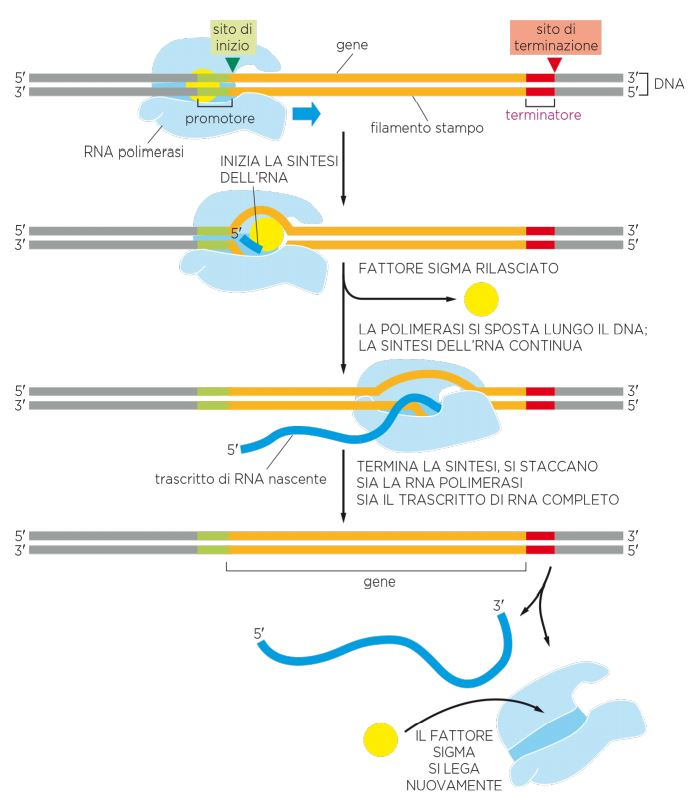
\includegraphics[width=0.4\textwidth]{images/trascrizioneProka.JPG}
            \caption{\small schema delle fasi della trascrizione procariotica}
            \label{fig:mesh1}
        \end{figure}
    
    \subsection{Trascrizione per eucarioti}
        Gli eucarioti hanno RNA-P differenti che assumono compiti specifici:
        \begin{itemize}
            \item RNA-P 1: trascrive la maggioranza del DNA ribosomiale 
            \item \textbf{RNA-P 2}: trascrive geni codificanti proteine 
            \item RNA-P 3: trascrive DNA ribosomiale 5s e tRNA
        \end{itemize}
        Vengono coinvolti altri \textit{transcription factor (TF)}, in particolare (TF II: opera con la RNA-P 2), quali 
        \begin{itemize} 
            \item TF IId è il più simile a $\sigma$ procariotico che utilizza una \textit{TATA binding protein} che si lega alla sequenza nucleotidica della TATA box (a monte della sequenza da trascrivere) che si lega al duplex per reclutare altri componenti specifici
            \item TF IIh: complesso multiproteico (di 9 subunità, compresa una che svolge attività elicasica) che determina la transizione da iniziazione a elongazione tramite attività enzimatica che modifica chimicamente una coda di RNA-P (fosforilazione con CDK7), quindi ne determina la processività.
        \end{itemize}
        Di seguito gli step della trascrizione per le cellule eucariotiche:
        \begin{enumerate}
            \item TF IId si attacca al DNA sulla sequenza specifica della TATA box che viene riconosiuta da TBP (TATA binding protein)
            \item distorsione del sito TATA
            \item formazione del complesso di iniziazione
            \item TF IIh espone il filamento stampo
            \item RNA-P comincia una fase di inizio abortivo (trascrive sequenze che poi vengono scartate fino ad arrivare alla conformazione finale)
            \item avviene la fosforilazione della quinta serina del CTD (ovvero il dominio C-terminale)
            \item RNA-P si stacca da TF IIh e inizia la fase di trascrizione
        \end{enumerate}
        \begin{figure}[h]
            \centering
            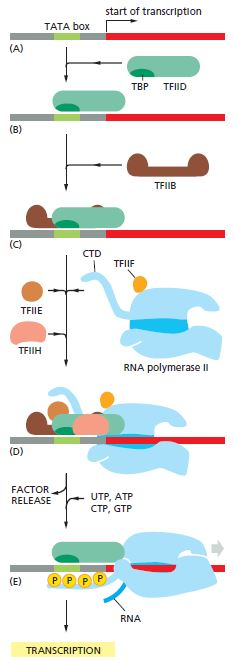
\includegraphics[width=0.3\textwidth]{images/trascrizioneEuka.JPG}
            \caption{\small schema delle fasi della trascrizione eucariotica}
            \label{fig:mesh1}
        \end{figure}
        
        \subsubsection{Maturazione dell'mRNA}
        L'RNA prodotto dalla trascrizione non è ancora pronto per essere utilizzato per la traduzione in proteine. Per la sua maturazione sono necessarie tre ulteriori fasi, ovvero l'apposizione di un capside all'estremità 5', la poliadenilazione all'estremità 3' e il "ritaglio" delle sequenze introniche (slicing). \\
            
            \textbf{Apposizione CAP:}
            Si tratta di una modifica chimica dell'estremità 5'. Viene apposta una metilguanosina da uno specifico enzima tramite un ponte trifosfato 5' - 5'. 
            Questa modifica avviene a livello cotrascrizionale, ovvero avviene durante la trascrizione, approssimativamente dopo circa 25b. Il cap che viene introdotto era precedentemente associato a RNA-P.\\
            
            \textbf{Poliadenilazione:}
            Si tratta di una modifica dell'estremità 3', avviene in contemporanea allo splicing dopo la fine della trascrizione (per ovvi motivi). Viene eliminata una piccola porzione di RNA e viene sostituito con uno stretch di sole adenine (150-250).\\
            Insieme alla presenza del cap in 5' segnala che l'RNA è maturo e pronto per la traduzione.
            
        \vspace{0.5cm}
        Apposizione del CAP e poliadenilazione comportano l'aumento della stabilità dell'RNA (molto instabile e minacciato da RNAasi) e sono necessari per l'esportazione dal nucleo.\\
            
            \begin{figure}[h]
                \centering
                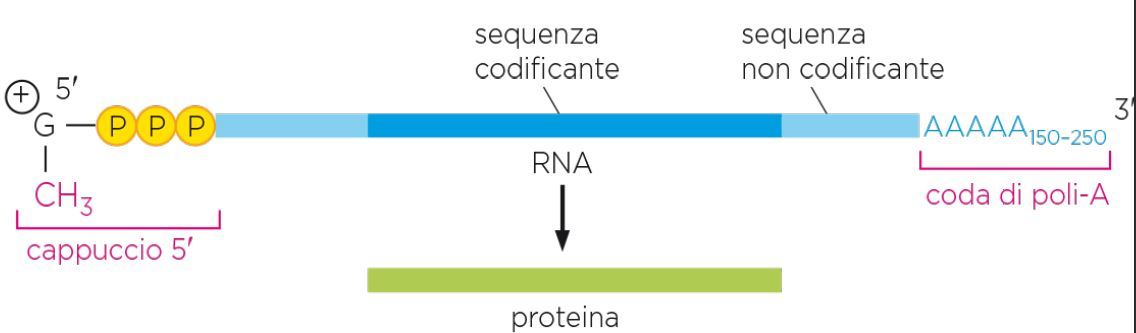
\includegraphics[width=0.5\textwidth]{images/poliAeCap.JPG}
                \caption{\small poliadenilazione e apposizione del CAP}
                \label{fig:mesh1}
            \end{figure}
            
            \textbf{Splicing:}
            Lo splicing è una procedura che avviene solo per gli organismi eucarioti. Infatti il trascritto di RNA contiene delle sequenze non codificanti chiamate \textit{introni}, più lunghe e frequenti di quelle codificanti (\textit{esoni}). 
            Lo splicing si occupa di eliminare queste sequenze lasciando nell'RNA maturo solamente gli esoni.\\
            Lo splicing è una modifica co-trascizionale che avviene tramite una transesterificazione.
            \begin{enumerate}
                \item in corrispondenza di una specifica adenina (solitamente prossima alla fine dell'introne), viene legato il gruppo OH all'estremità 5' del primo nucleotide dell'introne formando una conformazione a \textit{cappio}.
                \item le estremità degli esoni si ricongiungono
                \item viene eliminata la struttura a cappio intronica
            \end{enumerate}
            Un esone comincia sempre per G e finisce per AG, condizione necessaria perchè avvenga lo splicing.
            Un introne contiene sequenze non specifiche ma deve contenere una sequenza al 5' e al 3' specifica e una certa sequenza attorno alla adenina sulla quale avviene la transesterificazione. In particolare viene identificata come \textit{YUR\textbf{A}C}, dove Y sta per una pirimidina e R una purina.\\
            Questo processo è catalizzato da una ribonucleoproteina \textit{snRNP} (\textit{small nuclear ribonucleoprotein}) che si associano singolarmente alle estremità degli introni collaborando alla formazione del cappio e all'intervento di enzimi per lo splicing. \\
            Una volta che il cappio viene eliminato, gli RNA maturi possono formarsi anche cambiando l'ordine delle sequenze esoniche rimaste: questo processo è detto \textit{splicing alternativo} e dà luogo alla formazione di proteine differenti (processo regolato e specifico).
            A livello evolutivo, ci sono domini molto comuni tra proteine diverse e certi altri molto specifici. La modulabilità nella costruzione delle proteine (utilizzo ricorrente di sequenze introniche) aumenta la variabilità delle proteine in modo più efficacie e rapido.
            \begin{figure}[h]
                \centering
                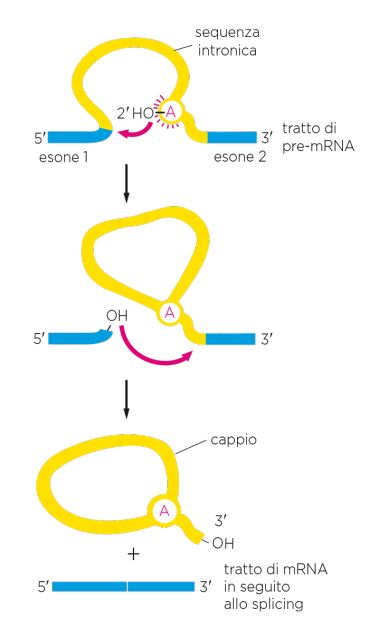
\includegraphics[width=0.4\textwidth]{images/splicing.JPG}
                \caption{\small splicing}
                \label{fig:mesh1}
            \end{figure}
            
        \subsubsection{Esportazione ed emivita}
            Per effettuare lo spostamento dell'mRNA maturo dal nucleo al citoplasma vengono coinvolte numerose proteine che si legano alla testa e alla coda dell'RNA. Ci sono anche complessi di giunzione tra gli esoni. Viene quindi effettuato un legame con il poro nucleare per l'esportazione. \\
            Le stesse proteine promuovono successivamente anche la traduzione. Le componenti che non passano attraverso il poro vengono degradate o riciclate. 
            La sequenza dell'mRNA viene comunque degradata in base alla sua emivita (determinata da sequenze interne codificanti, contribuisce a quest'informazione anche la sequenza in 3' dell'UTR, ovvero \textit{untranslated region}, URT è presente anche al 5'). Dall'emivita dipende il numero di proteine prodotte da quel singolo stretch di mRNA. 

\section{Traduzione}
    Si parla di \textit{traduzione} perchè si passa dal linguaggio nucleotidico a quello AA. Risulta necessario leggere nucleotidi a gruppi di tre in modo da poter riuscire ad identificare univocamente tutti i 20 AA ($4^{3} = 64$ sequenze differenti). Un AA può corrispondere a più triplette (o codoni), tre specifici codoni identificano lo stop alla traduzione.
    Codoni diversi che identificano uno stesso AA sono più variabili all'ultimo nucleotide rispetto agli altri.
    \subsection{Moduli di lettura}
        Ogni proteina comincia con una Metionina, identificata univocamente da AUG (per i mitocondri anche AUA) e finiscono inderogabilmente con una codone di stop (UAA, UAG, UGA). Metionina e stop si possono vedere come elementi di punteggiatura.\\
        Non tutte i nucleotidi dell'mRNA messaggero codificano per AA (per esempio URT citati prima).\\
        Il ribosoma comincia a tradurre la proteina nel momento in cui trova la sequenza AUG per la metionina. Da quel momento legge a gruppi di tre i nucleotidi associando ad ogni tripletta l'AA corretto.
        \subsubsection{Esperimento storico}
            Storicamente, per individuare a quale codone fosse associato quale AA, si creava artificialmente uno stretch di nucleotidi successivo a un mRNA "originale". Per esempio utilizzando uno stretch di U e fornendo questo mRNA sintetico a una cellula, si notava che venivano prodotte fenilalanine. Facendo la stessa cosa con altre sequenze note si riuscirono a dedurre alcuni codoni.\\
            Utilizzando successivamente sequenze di UGUG... alternate si ottiene una sequenza di cisteina e valina, non c'è modo però di sapere se UGU codfichi per l'una o per l'altra.\\
            Successivamente si utilizzarono i tRNA per dedurre la decodifica precisa, da un lato sono coniugate a un AA, dall'altro si associano complementarmente al codone di mRNA. In particolare si utilizzarono delle triplette sintetiche che portarono alla decodifica delle associazioni nucleotidi-AA.
            
    \subsection{tRNA}
        I tRNA sono composti da circa 80 nucleotidi e alla loro estremità in 3' si legano a un AA specifico. Ha una tipica forma a trifoglio e nell'ansa dell'anticodone mostra una sequenza complementare al codone che codifica per l'AA legato al tRNA.\\
        La sua sequenza nucleotidica può contenere basi non canoniche. \\
        I tRNA sono al massimo 61 differenti (64 - 3 codoni di stop), ma il numero minimo è 31. L'uomo possiede solamente 48 tRNA differenti.\\
        La base in posizione 3 è la più variabile (le triplette differenti che codificano per lo stesso AA sono generalmente differenti per il nucleotide in posizione 3). La base azotata \textit{ipoxantina} può comparire in posizione 3 e rappresentare una wildcard per A, C e U. In terza posizione possono esserci anche appaiamenti \textit{wabble} (ad esempio a una C può essere associata una G o una U).
        \begin{figure}[h]
                \centering
                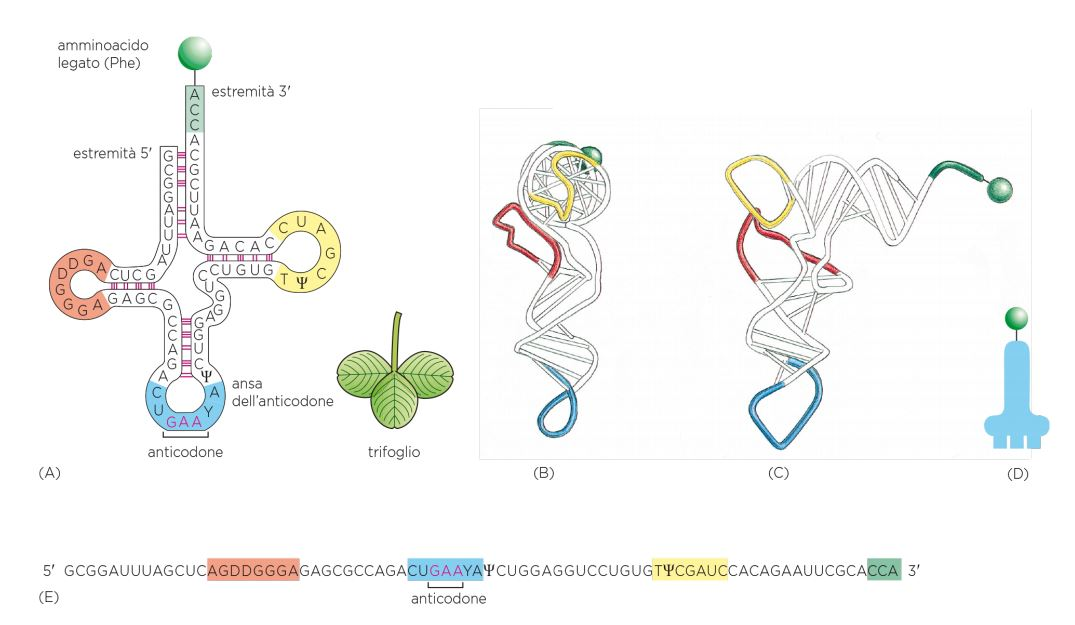
\includegraphics[width=0.5\textwidth]{images/tRNA.JPG}
                \caption{\small tRNA}
                \label{fig:mesh1}
        \end{figure}
    
        \subsubsection{Associazione AA a tRNA}
            Più di un legame ad alta energia viene utilizzato per "caricare" l'AA sul tRNA da una specifica \textit{tRNA sintetasi} per ogni AA. 
            Ogni tRNA sintetasi deve saper riconoscere sequenze di codoni differenti per lo stesso AA e forma un legame estere tra i due. Per il riconoscimento viene utilizzata la sequenza del braccio del trifoglio. 
         
    \subsection{Ribosomi}
        Sono macro-complessi ribonucleoproteici che possono essere libere nel citoplasma o essere associati a RE. Sono formati da 80 proteine differenti e 4 molecole di rRNA. Sono composti di una subunità maggiore (circa 50 peptidi e 3 molecole di rRNA) e una inferiore (circa 30 peptidi e 1 molecola di rRNA). Sulla subunità minore è presente un sito per l'associazione del mRNA.\\
        Tra le due subunità sono presenti tre tasche specifiche (quindi per tre codoni contemporaneamente): E, exit per il rilascio; P, peptidil tRNA e A, amminoacil tRNA. Questi siti coinvolgono sia la subunità maggiore che quella minore. 
        \begin{figure}[h]
                \centering
                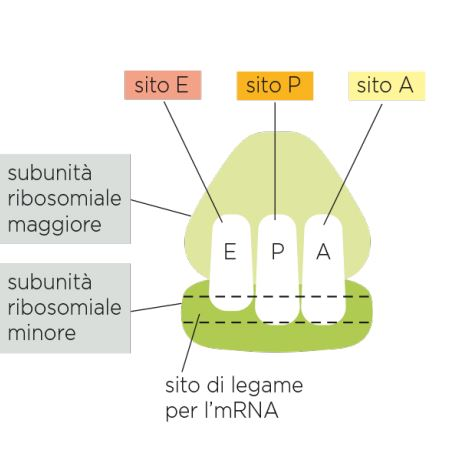
\includegraphics[width=0.35\textwidth]{images/ribosoma.JPG}
                \caption{\small struttura ribosoma}
                \label{fig:mesh1}
        \end{figure}
        Il robozima è la porzione a RNA con funzione catalitica presente del ribosoma che si occupa effettivamente della sintesi proteica, ovvero la \textit{peptidiltransferasi} presente internamente alla subunità maggiore del ribosoma. Strutturalmente è simile a un classico enzima proteico (esiste tasca per favorire la reazione) per orientare i reagenti.
        \subsubsection{Nucleoli}
            Sono domini del nucleo che sintetizzano gli rRNA, tramite RNA-P 1 e 3. C'è una densità di cromatina completamente differente (facilmente osservabili al microscopio) e vengono \textit{clusterizzate} diverse sequenze per il rRNA (cromosoma 1 per rRNA 5s e cromosomi 13, 14, 15, 21 e 22 per rRNA 47s).
    
    \subsection{Processo di traduzione}
        \subsubsection{Inizio per procarioti}
            L'mRNA procariotico maturo non possiede un cap su 5'.
            Esistono sequenze specifiche a cui il ribosoma si associa e comincia la traduzione. Lo stesso mRNA può produrre proteine diverse qualora i ribosomi comincino da AUG differenti (metionine). Gli mRNA batterici che codificano per più geni vengono detti \textit{policistronici}.
        
        \subsubsection{Inizio per eucarioti}
            \begin{enumerate}
                \item La subunità minore si associa ad elementi proteici e a un tRNA iniziatore specifico (che trasporta metionina, riconosce AUG). Esistono due tipi di tRNA per la metionina: uno che viene utilizzato per l'inizio della traduzione e uno per l'inserimento generico di una metionina nella sequenza AA.
                \item Questo complesso si lega all'estremità 5' (riconosciuta dal cap).
                \item Il complesso scorre in direzione 3' fino a trovare il codone AUG per la metionina. Questo evento determina un arresto e quindi il modulo di lettura delle triplette.
                \item I fattori di iniziazione si dissociano e interviene la subunità maggiore del ribosoma per cominciare l'elongazione.
            \end{enumerate}
            Nella maggior parte delle proteine non si riscontra una metionina all'N terminale perchè tramite modifiche post traduzionali vengono spesso rimosse.
            
        \subsubsection{Elongazione}
            \begin{enumerate}
                \item Due tRNA sono ora adiacenti nelle tasche P ed A all'interno del ribosoma. In posizione P, l'AA è legato alla catena peptidica. In posizione A è presente il tRNA che ha portato il nuovo AA da legare al peptide.
                \item Una componente catalitica promuove la formazione del legame peptidico tra l'AA in P e quello in A (reazione catalitica). 
                \item Avviene uno slittamento della subunità maggiore (il sito P diventa E, il sito A diventa P, A rimane vuoto). 
                \item Avviene uno slittamento della subunità minore. Il tRNA che ora era nel sito E viene rilasciato.
                \item Subentra un nuovo tRNA che si associa al codone.
            \end{enumerate}
            Anche la scansione del mRNA avviene dal 5' al 3', per questo abbiamo anche una direzione di sintesi e lettura degli AA (da N a C terminale).\\
            Durante la fase di elongazione avviene anche il folding della proteina. Possono esserci degli chaperon associato al ribosoma. La velocità di sintesi della proteina ha impatto sulla sua conformazione tridimensionale. I tRNA specifici per un codone sono disponibili in quantità differenti, quindi il codone richiesto determina la velocità della sintesi. \\
            Anche gli mRNA possono essere tradotti da poliribosomi, ossia molteplici ribosomi associati allo stesso stretch che traducono la stessa proteina "in fila". Esistono molecole usate come antibiotici che inibiscono la traduzione batterica che non hanno tossicità per i meccanismi umani.
    
        \subsubsection{Terminazione}
            I tRNA antiparalleli ai codoni di stop sono associati a fattori di rilascio.
            \begin{enumerate}
                \item Il sito A contiene una sequenza di stop
                \item Il fattore di rilascio associato al tRNA si lega e cambia conformazione del sito catalitico. Idrolizza il legame tra l'ultimo AA e il suo tRNA rilasciando la proteina neosintetizzata libera. 
                \item Il ribosoma e gli altri fattori si dissociano.
            \end{enumerate}
        
        \begin{figure}[h]
                \centering
                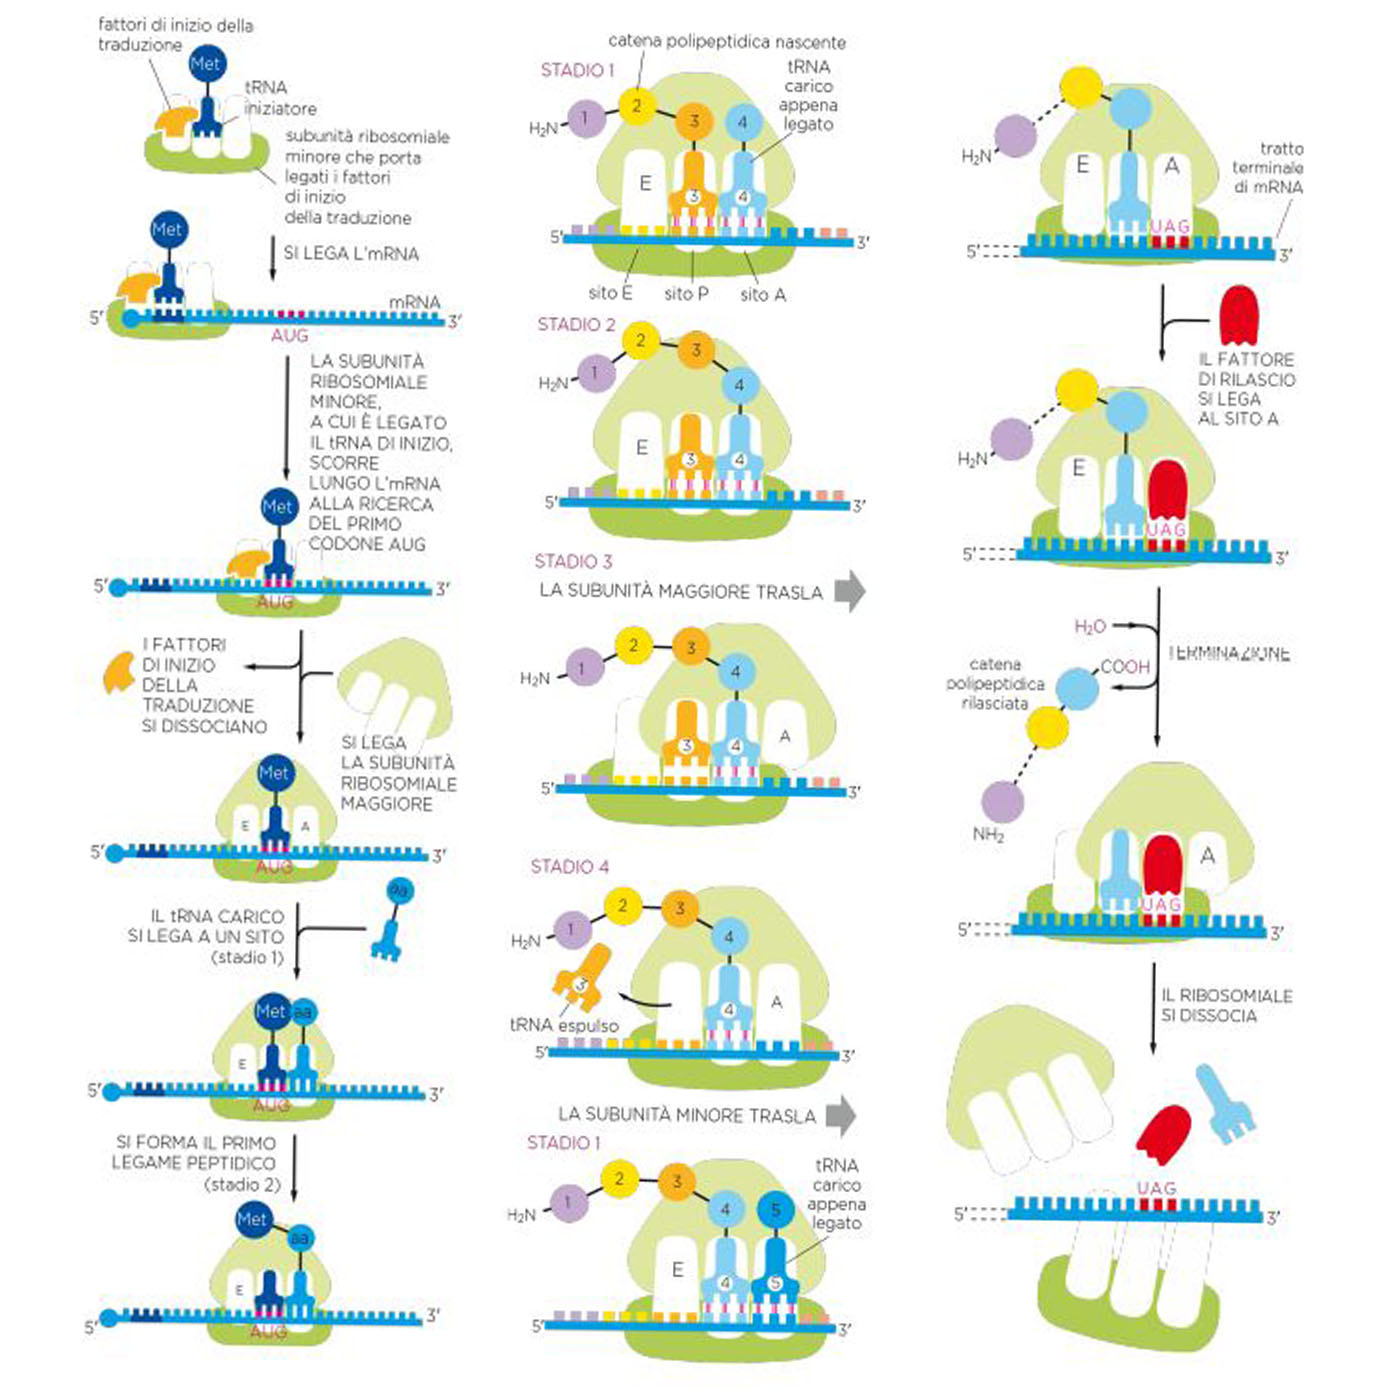
\includegraphics[width=1\textwidth]{images/traduzione.jpg}
                \caption{\small fasi della traduzione, rispettivamente iniziazione, elongazione e terminazione per gli eucarioti}
                \label{fig:mesh1}
        \end{figure}
        
        \subsubsection{Post traduzione e morte}
            Le proteine possono subire delle modifiche post-traduzionali, ne si può modificare l'emivita e di conseguenza la sua concentrazione. \\
            Un polipeptide che finisce il suo ciclo di vita viene "spezzettato" nel proteasoma, un core catalitico che svolge il polipeptide (consumando ATP) e rilascia AA singoli o bipeptidi nel citoplasma.\\
            L'ubiquitina è un marker per le proteine che devono essere degradate, l'aggiunta molteplici catene di questa proteina (composta di 76 AA) è anche essa una modifica post-traduzionale chiamata \textit{poliubiquitinazione} e viene effettuata sempre su una lisina.\\
            Il proteasoma riconosce le sequenze di ubiquitina e degrada la proteina.\\ 

\pagebreak
\setcounter{section}{0}

\large{\addcontentsline{toc}{part}{Capitolo 6: Citoscheletro}}
\Huge\textbf{Capitolo 6: \\Citoscheletro}

\vspace{1cm}
\small
Il citoscheletro è una struttura cellulare composta da microtubuli (MT), filamenti intermedi (FI) e microfilamenti (MF). Hanno funzioni, dimensioni e composizioni molecolari differenti.

\section{Microtubuli}
    I MT hanno un diametro di circa 25 nm e sono l'"impalcatura" per il traffico intracellulare. Sono presenti in ogni tipologia cellulare e hanno struttura sempre uguale a se stessa, ma assumono funzioni differenziate.
    \subsection{Struttura e conformazioni}
        Un MT è un cilindro cavo composto da 13 protofilamenti lineari con simmetria radiale. I protofilamenti sono eterodimeri composti da sequenze alternate di $\alpha$tubulina ($\alpha$T) e $\beta$tubulina ($\beta$T). $\alpha$T si associa sempre a GTP (funzione di cofattore) mentre $\beta$T si può associate a GTP o GDP (funzione di cofattore) e catalizza eventualmente l'idrolisi da GTP a GDP.
        \begin{figure}[h]
            \centering
            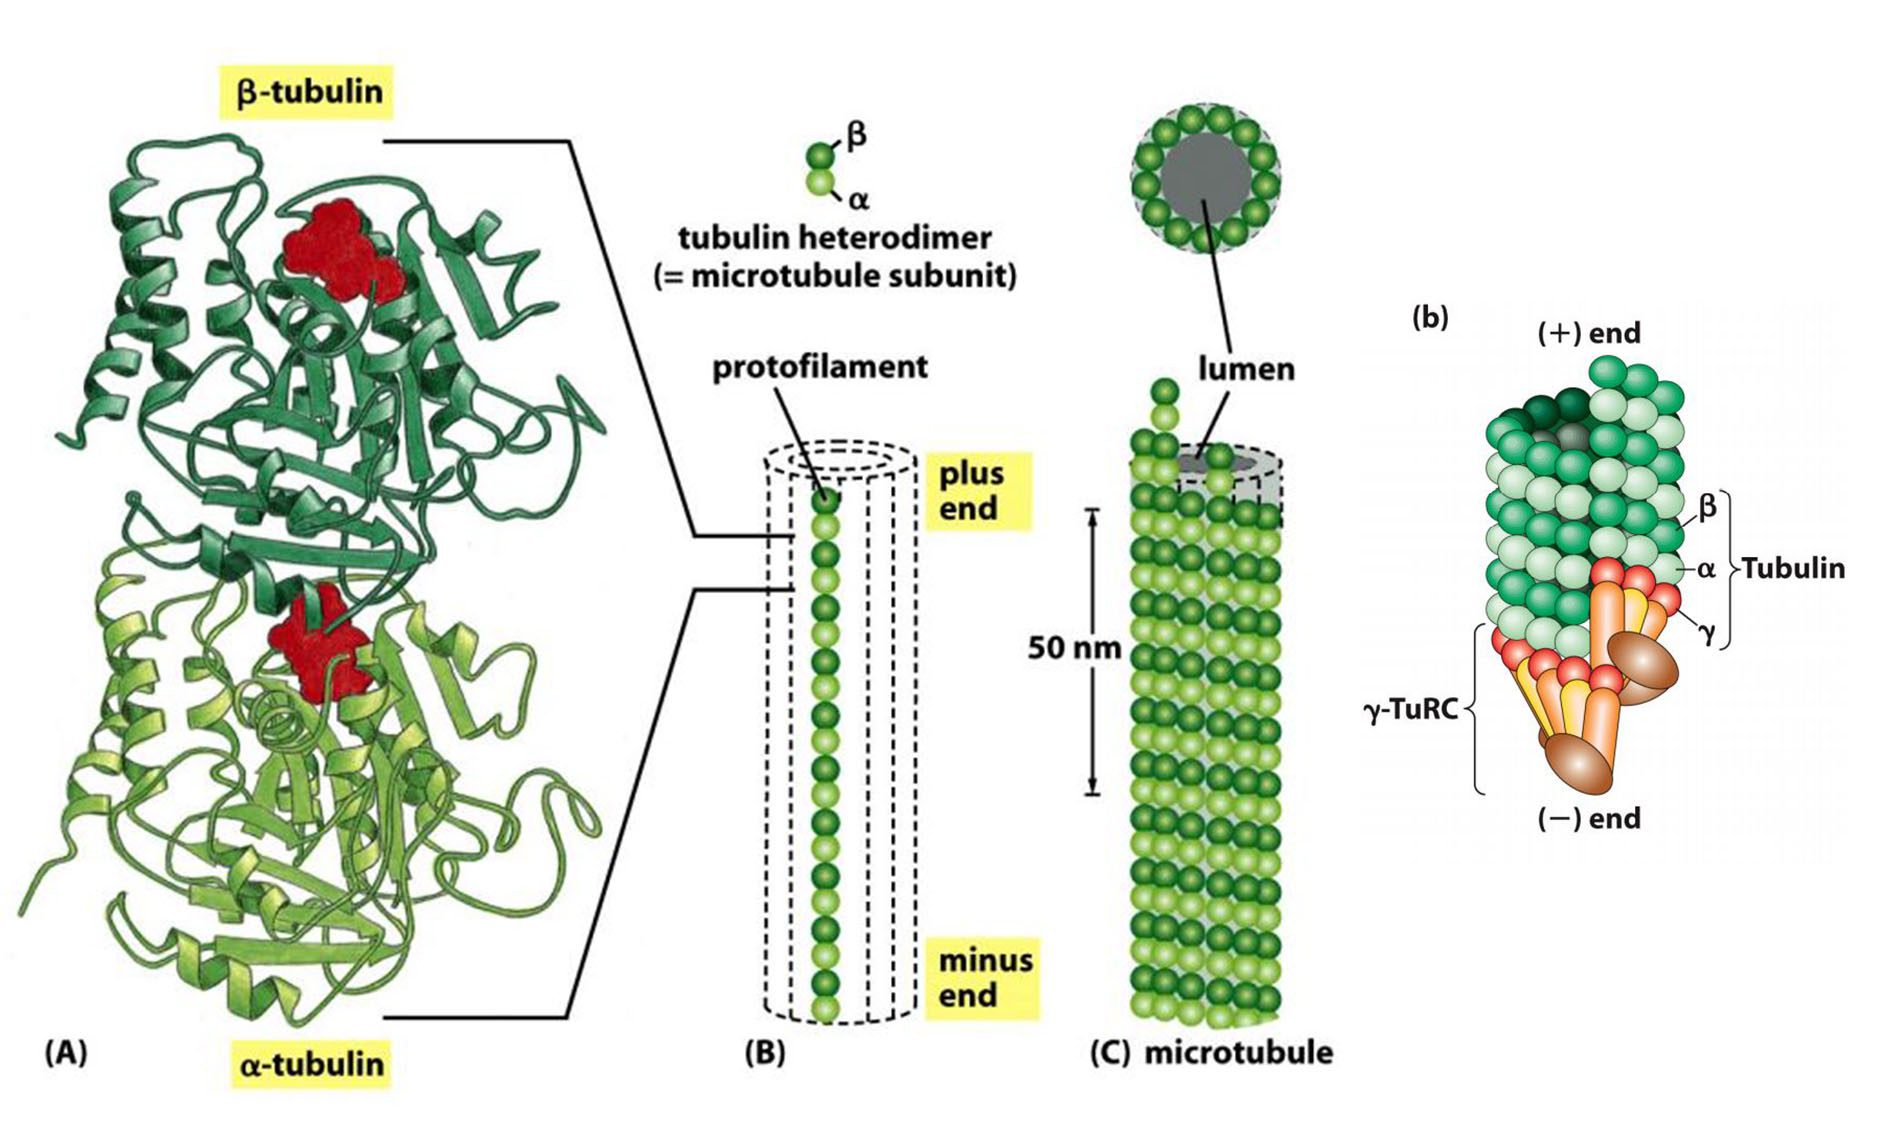
\includegraphics[width=0.8\textwidth]{images/MT.JPG}
            \caption{\small struttura di un microtubulo}
            \label{fig:mesh1}
        \end{figure}
        I protofilameti sono eterodimeri orientati ($\alpha$T , negativa - $\beta$T, positiva) quindi intrinsecamente polari. I MT sono composti da 13 protofilamenti per la formazione di un cilindro cavo (la polarità del MT corrisponde alla polarità del protofilamento, i fasci sono paralleli e hanno la stessa polarità). L'andamento elicoidale fa sì che si verifichi una discontinuità chiamata seam visibile come stacco del pattern.    \\
        I MT possono assumere più strutture:
        \begin{itemize}
            \item singola: solamente un tubulo di 13 protofilamenti
            \item doppiette: un tubulo da 13 filamenti e uno da 10 
            \item triplette: un tubulo da 13 e due da 10
        \end{itemize}
        L'estremità negativa del MT è "incappucciata" a un cap chiamato $\gamma$TURC (\textit{tubulin ring complex}), un complesso formato da 14 molecole di $\gamma$ tubulina ($\gamma$T). L'ultima $\alpha$T è associata ad una $\alpha$T che lega GTP.
        Questo protegge l'estremità negativa e favorisce associazioni con altre proteine che predispongono alla nucleazione.
        \subsubsection{MTOC}
            I MT possono assumere conformazioni spaziali molto diverse, sempre polari con l'estremità negativa sempre associata ad un MTOC. (\textit{microtubule-organizing center}). In ogni cellula è sempre presente almeno un MTOC. Esempi di MTOC sono il centrosoma e il corpo basale di un cilio.\\
            Gli MTOC organizzano la conformazione spaziale della cellula e degli organelli. La densità dei MT aumenta in prossimità di un MTOC.\\
            
                \textbf{Centrosoma}\\
                Il centrosoma è il principale MTOC e al contempo un organello proteico senza membrana circondato da PCM (\textit{peri centriolar material}) contenente $\gamma$TURC. Ciascun centrosoma è composto da due centrioli disposti perpendicolarmente.\\
                Il centrosoma è composto di due centrioli così strutturati:
                \begin{itemize}
                    \item all'estremità basale sono presenti triplette di MT
                    \item all'estremità distale sono presenti doppiette di MT
                \end{itemize}
                Sono sempre composti di 9 triplette di MT equidistanti tra loro. Uno dei due centrioli è più vecchio e si dice \textit{madre} ed è morfologicamente diverso dal secondo. 
                Il centriolo madre ha nelle porzioni distale e sub-distale degli appendici. Il centriolo figlio non porta appendici ma presenta un \textit{cartwheel} nella porzione basale e ogni raggio della ruota lega una tripletta di MT. Il cartweel è una struttura transitoria che concorre alla formazione del centriolo (quindi utile alla fase iniziare della sintesi).\\
                Non è noto perchè sia necessario un organello così complesso per legare la $\gamma$T delle estremità negative dei MT.\\
                Le cellule vegetali non presentano centrioli, ma esistono altre forme di MTOC.\\
                Normalmente una cellula presenta un unico centrosoma. In fase di duplicazione viene anche esso duplicato ed è funzionale alla separazione della cellula, alla citochinesi e alla cariochinesi.
                \begin{figure}[h]
                    \centering
                    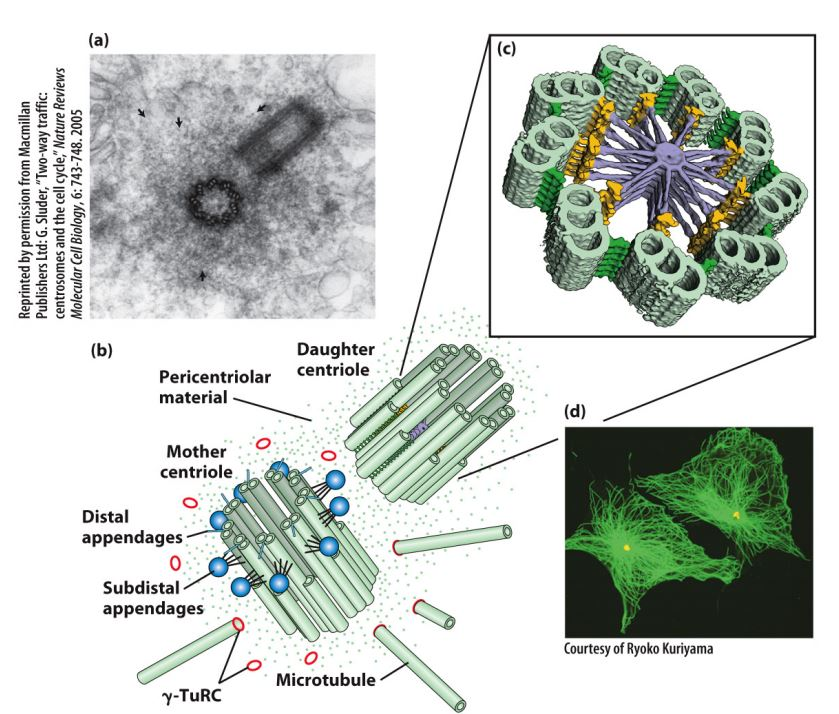
\includegraphics[width=0.5\textwidth]{images/centrosoma.JPG}
                    \caption{\small struttura di un centrosoma} 
                    \label{fig:mesh1}
                \end{figure}\\
                Il centrosoma assume ruoli differenti a seconda della fase cellulare:
                \begin{enumerate}
                    \item in fase di duplicazione forma organizza il fuso mitotico
                    \item può formare il corpuscolo basale per il cilio primario
                \end{enumerate}
                Il centriolo madre presenta gli appendici distali e sub-distali necessari per diventare basal body e nucleare il cilio.
        
    \subsection{Comportamento nella cellula}
        \subsubsection{Instabilità dinamica dei MT}
            Tra le estremità positive e negative dei MT affiora un'asimmetria: l'estremità positiva infatti accresce più velocemente di quella negativa. Studi in vitro suggeriscono che dopo una certa soglia, il MT depolimerizza (in base alla torbidità).\\
            In vitro, i dimeri di tubulina si associano in due direzioni. I legami longitudinali sono per lo più stabili, mentre quelli laterali soffrono grave instabilità nel momento in cui avviene una curvatura del MT dovuta alla presenza di GDP (se la curvatura è troppo pronunciata si verifica una catastrofe). Esistono farmaci che rendono le catastrofi più frequenti con il fine di danneggiare un tessuto tumorale.\\
            Si nota inoltre che fornendo i dimeri di tubulina, essi si associano spontaneamente nella formazione di un MT, sempre con la stessa organizzazione spaziale.\\
            
            \textbf{Catastrove}\\
                Si osserva in vitro una ritmica crescita e decrescita del MT, le seconde dovute alle cosiddette \textit{catastrofi}, durante le quali la velocità di decrescita supera quella della crescita.
                All'interno di una cellula succede lo stesso fenomeno, per ogni MT gli eventi sono asincroni e indipendenti.
                Il MT si associa stabilmente utilizzando GTP sia per $\beta$T che per $\alpha$T. Qualora il GTP associato alla $\beta$T venga idrolizzato, avviene un lieve cambio conformazionale che tende a incurvare il protofilamento. Questo evento favorisce la depolimerizzazione, quindi avviene una catastrofe.\\
                
            \textbf{Rescue}\\
                Alle catastrofi si alternano fasi di \textit{rescue}, durante le quali il GDP viene sostituito da GTP (processo endoergonico) per la costruzione di MT stabili.\\
            
            L'alternare di catastrofi e rescue definiscono l'instabilità dinamica intrinseca dei MT.
            \begin{figure}[h]
                    \centering
                    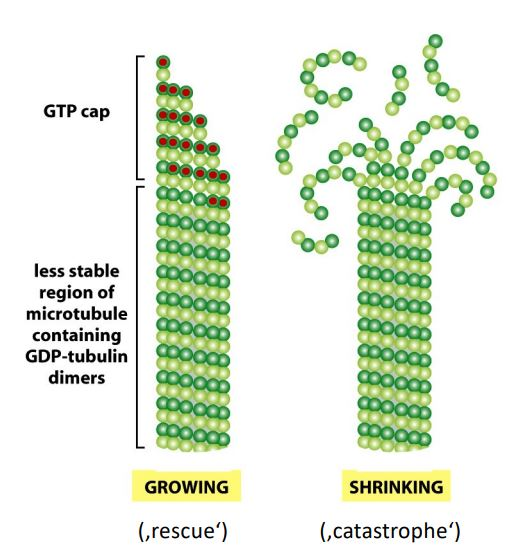
\includegraphics[width=0.5\textwidth]{images/rescue_catastrofe.JPG}
                    \caption{\small schema degli eventi di catastrofi e rescue}
                    \label{fig:mesh1}
            \end{figure}
            Quando viene idrolizzato GTP a GDP, non avviene una catastrofe immediatamente, bensì si crea una tensione del MT che viene sfruttata dalla cellula per muovere componenti cellulari o cercare altre componenti (ad esempio, esistono delle proteine che si associano specificamente all'estremità positiva in fase di depolimerizzazione per essere trascinate verso l'estremità negativa).\\
            Inoltre la stessa crescita e decrescita dinamica è sfruttata per "cercare" componenti, infatti la posizione centrale dei centrosomi e la possibilità di crescita e decrescita delle sue estremità positive, fanno sì che (anche stocasticamente) queste vengano in contatto con organelli o generalmente componenti cellulari (comprese proteine della membrana). Quindi hanno anche il compito di posizionare gli organelli.
                
        \subsubsection{Treadmilling}
            Il MT in vitro tende a polimerizzare all'estremità positiva mentre all'estremità negativa si nota una depolimerizzazione. Questo avviene meno frequentemente nelle condizioni normali della cellula perchè è presente all'estremità negativa $\gamma$TURC che protegge l'estremità.\\
            Il processo di depolimerizzazione all'estremità negativa e polimerizzazione a quella positiva favorisce una certa dinamicità, lo "scorrimento" del filamento si chiama appunto \textit{treadmilling}.
            
        \subsubsection{MAPS}
            Le MAPS (\textit{microtubule associated proteins}) modificano il comportamento dei MT.\\
            
            \textbf{TAU}\\
                TAU interagisce con i dimeri di tubulina (con domini specifici) elettrostaticamente per ne determina la distanza reciproca in base alla lunghezza di domini che protrudono dalle TAU stesse (lunghezza del dominio di TAU è inferiore a MAP2, ad esempio).\\
                
            \textbf{EB1}\\
                EB1 (end-binding protein) si lega alle estremità positive (in particolare il GTP cap). Tipicamente è associata ad altre proteine che sfruttano EB1 per essere trasportate (grazie l'instabilità dinamica).\\
                
            \textbf{Chinesina 13 (CHI13)}\\
                Altera il comportamento dei MT catalizzando l'energia per dissolvere il MT a livello del dimero (quindi promuove una catastrofe).\\
                
            \textbf{Stathmin}\\
                Hanno una conformazione a U con affinità per gli eterodimeri di $\alpha$T e $\beta$T. Nel momento in cui l'estremità positiva sia incurvata ne accentuano questa caratteristica.
        
    \subsection{Motor proteins}
        Le \textit{motor proteins} sono le proteine che sono associate al movimento di molecole o complessi maggiori lungo i MT.
        
        \subsubsection{Esperimenti}
            Marcando degli AA con radioattività, si nota come la proteina costruita con questo AA venga trasportata lungo i MT in verso sia anterogrado che retrogrado. Si nota inoltre che la velocità del trasporto è più alta rispetto al semplice trasporto in soluzione. Si deduce che ci sono delle componenti che si occupano del movimento di queste molecole (ovvero le motor proteins).\\
            Utilizzando l'assone gigante del calamaro, è possibile estrarre fasci di MT ed è possibile notare che le vescicole viaggiano lungo questo canale in senso anterogrado e retrogrado.
        
        \subsubsection{Chinesine}
            Sono una famiglia di motor proteins che si muovono per lo più dall'estremità negativa a quella positiva (tranne rare eccezioni), quindi in senso anterogrado. La prima scoperta è stata isolata dall'assone gigante del calamaro, ovvero CHI1.\\
            
            \textbf{Struttura} \\
                Le chinesine sono composte da due catene pesanti (stelo), due catene leggere, due teste e due code. \\
                Sulle teste è presente un nucleoside di-fosfato. Sono proprio le teste che interagiscono con il MT per "camminare".\\
                Trasportano un cargo tramite dei legami con le catene leggere attraverso in recettore per la CHI presente sul cargo.\\
            
            \textbf{Classificazione}\\
                Le chinesine (CHI) sono divise in 14 classi differenti, codificare da 45 geni diversi (nel genoma umano). La struttura della testa resta per lo più simile tra le classi, altri domini presentano un'elevata eterogeneità.
                \begin{figure}[h]
                    \centering
                    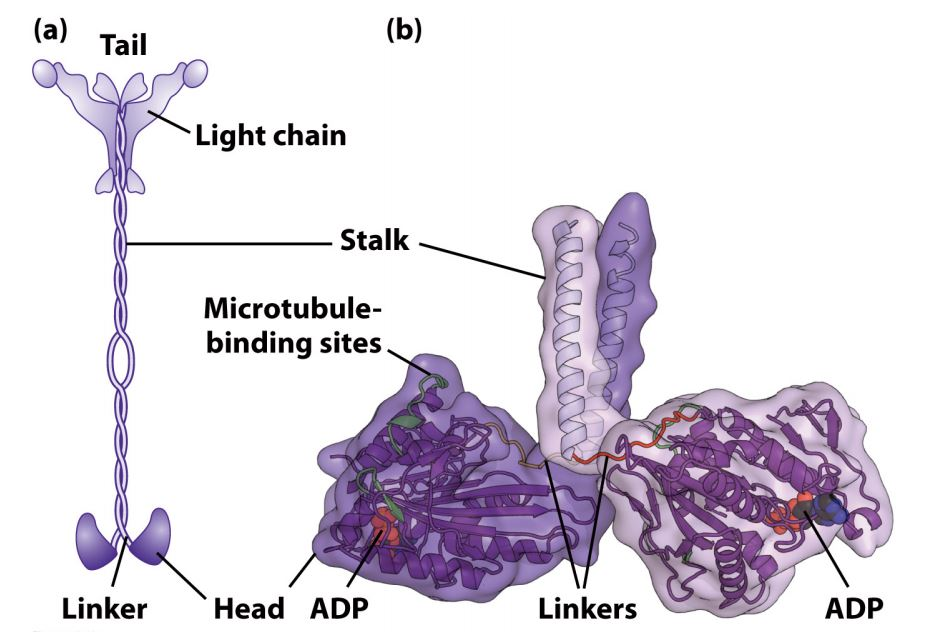
\includegraphics[width=0.5\textwidth]{images/chinesina.JPG}
                    \caption{\small chinesina 1}
                    \label{fig:mesh1}
                \end{figure}
                \begin{itemize}
                    \item Chinesina 1 (CHI1) è un eterodimero, la più classica rappresentata in figura
                    \item Chinesina 2 (CHI2), è un eterotrimero (due catene pesanti diverse che si associano a un terzo polipeptide che determina inetrazione con il cargo).
                    \item Chinesina 5 (CHI5), un tetrametro formato da due coiled coil e quattro piedini. Forma contatti con due MT ed è per questo utilizzato nei processi che necessitano di sliding (entrambe le coppie scorrono nello stesso verso).
                    \item Chinesina 13 (CHI13), è un dimero di cui la quasi totalità è rappresentata dai piedini (non hanno uno stelo). Non è destinato al movimento ma alla catalizzazione della depolimerizzazione dei MT.
                \end{itemize}
                
            \textbf{Movimento}\\
                Il movimento delle CHI è dovuto all'idrolisi di un ATP per ogni "passo" (16 nm, ovvero la distanza tra due dimeri di $\alpha$T e $\beta$T).
                Chiamiamo per chiarezza i due piedini $x$ e $y$. 
                \begin{enumerate}
                    \item Il piede $x$, ora posto davanti (leading head), verso la direzione target, non è legato a nucleotidi: per questo motivo è saldamente legata al MT. $x$ lega un ATP, il quale ingresso induce un irrigidimento che promuove il movimento dei $y$.
                    \item Il piede $y$, posto dietro (trailing head), possiede un ATP che idrolizza ad ADP per allentare il suo legame con MT. Essendo $x$ saldamente legato al MT e quindi svolge la funzione di perno, $y$ arriva in posizione anteriore diventando leading head.
                    \item  $y$ ora si trova ad essere la trailing head e per rafforzare il legame al MT espelle ADP. Quindi il ciclo ricomincia.
                    \item La CHI non si dissocia mai dal MT quindi ha un comportamento processivo.
                \end{enumerate}
                La CHI non si dissocia mai dal MT quindi ha un comportamento processivo.
                \begin{figure}[h]
                    \centering
                    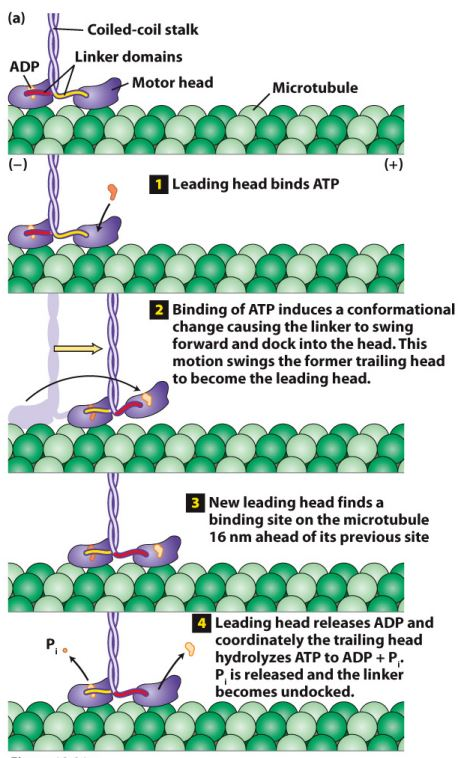
\includegraphics[width=0.5\textwidth]{images/chinesinMovement.JPG}
                    \caption{\small movimento della chinesina}
                    \label{fig:mesh1}
                \end{figure}\\
                
            \textbf{Conformazioni}\\
                Le CHI possono assumere delle conformazioni attive o inattive.\\
                Le conformazioni attive legano in cargo e un MT.
                Le conformazioni inattive sono tali per cui la CHI si ripiega su se stessa. In questo modo si inibisce la funzione catalitica e la proteina viene trasportata da un altro agente all'estremità negativa per poter essere nuovamente utilizzata.
            
        \subsubsection{Dineine}
            Le dineine (DIN) sono proteine di trasporto molto più grandi delle CHI, che solitamente si muovono dall'estrermità positiva a quella negativa (senso retrogrado). \\
            Si differenzia tra DIN citoplasmatica e flagellare.\\
            
            \textbf{Struttura}\\
                Essendo la DIN una molecola molto grande, non è ancora del tutto noto il suo comportamento e la sua struttura.\\
                Sono formate da una catena pesante, una catena leggera e una catena intermedia. La catena pesante è composta da più di 4000 AA (supera i 550 kDalton).\\
                Le DIN hanno delle teste che svolgono attività ATPasica: sono dei conglomerati di sei domini proteici che formano un anello che in termini strutturali è costituito da AAA ATPasi. Il ripiegamento di questo polipeptide fa si che si generino i gambi per protrusione per formare la testa della DIN.\\ 
                Due copie di questo polipeptide formano due "piedini" per camminare sui MT.\\
                Il "cammino" della DIN è dovuto a un cambio conformazione che consiste in un cambio dell'angolo tra lo stelo e l'esamero.\\
                
            \textbf{Interazione con il cargo}\\
                Le DIN interagiscono con un complesso chiamato \textit{dinactina} che concorre a stabilire interazioni con il cargo. La sua subunità \textit{dinamitina} stabilisce l'interazione tra DIN e dinactina. Anche DIN lavora in maniera processiva.
                \begin{figure}[h]
                    \centering
                    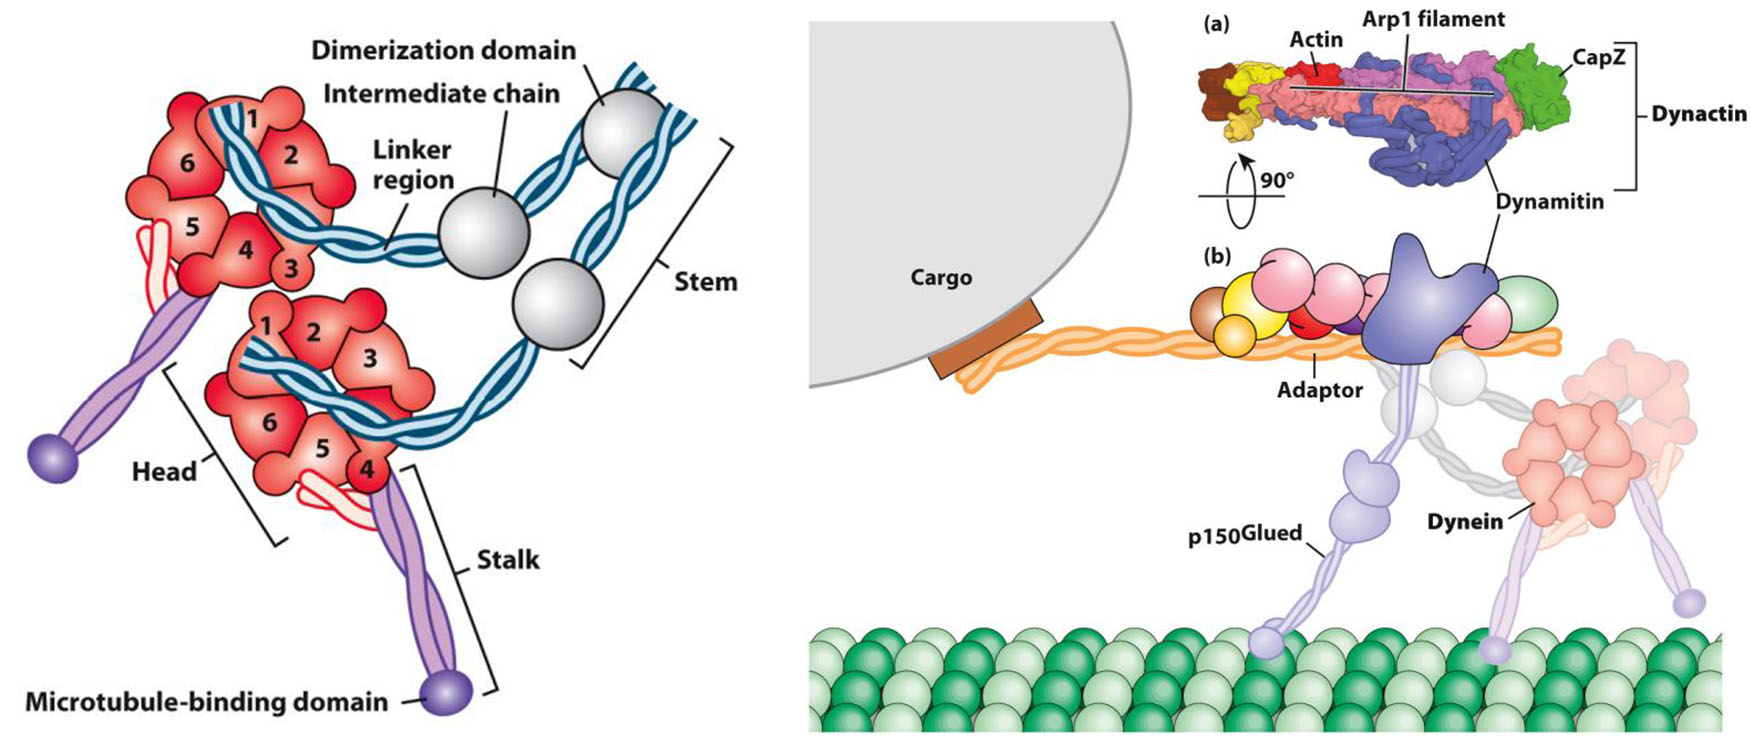
\includegraphics[width=1\textwidth]{images/dineina.JPG}
                    \caption{\small a sinistra struttura della dineina, a destra l'interazione con il cargo}
                    \label{fig:mesh1}
                \end{figure}
                
        \subsection{Interazioni e modifiche}
            Organelli differenti interagiscono con motor proteins diverse. In base a ciò si definiscono strutture e disposizioni differenti interne alla cellula.\\
            I melanofori (cellule dell'epidermide di rettili e pesci), contengono vescicole (melanosomi) con pigmenti che modificano il colore in base alla loro posizione, dettata per l'appunto dal movimento sui MT dei melanosomi.\\
            
            $\alpha$T e $\beta$T possono subire modifiche post-traduzionali. In particolare possiamo assistere a:
            \begin{itemize}
                \item poli glutammilazione sia per $\alpha$T che per $\beta$T che ne promuove la stabilità
                \item poli glicinazione sia per $\alpha$T che per $\beta$T che ne promuove instabilità\\
                Poli glutammilazione è mutualmente esclusivo rispetto a poli glicinazione.
                \item detirosinilizzazione per $\alpha$T che determina la propensione per la CHI13 a depolimerizzare il MT (con questa modifica sono più resistenti alla depolimerizzazione)
                \item acetilazione della lisina per $\alpha$T presenti all'interno della struttura nel caso di cilia o flagelli
            \end{itemize}
            Combinazioni di modifiche determinano comportamenti diversi (CHI1 si associa preferibilmente con MT detirosinati e acetilati).
        
    \subsection{Cilia e flagelli}
        Sono protrusioni costituite in gran parte da MT ricoperte da membrana (e ne richiedono la presenza per resistere). 
        \subsubsection{Struttura}
            Sono costituite da una porzione basale che contiene l'MTOC (un corpo basale, è effettivamente un centriolo) composto da nove triplette e la ruota solitamente presente nel centriolo figlio. Da qui vengono nucleate doppiette di MT. Ha due MT centrali.\\
            C'è una zona di transizione che funge da filtro tra parte interna ed esterna.
            Per assonema si intende la protrusione che può avere lunghezze molto variabili (da micrometri a millimetri). 
            La nessina connette le doppiette di MT, le strutture a raggio conferiscono rigidità, all'interno sono sempre presenti i due MT singoli.
            \begin{figure}[h]
                \centering
                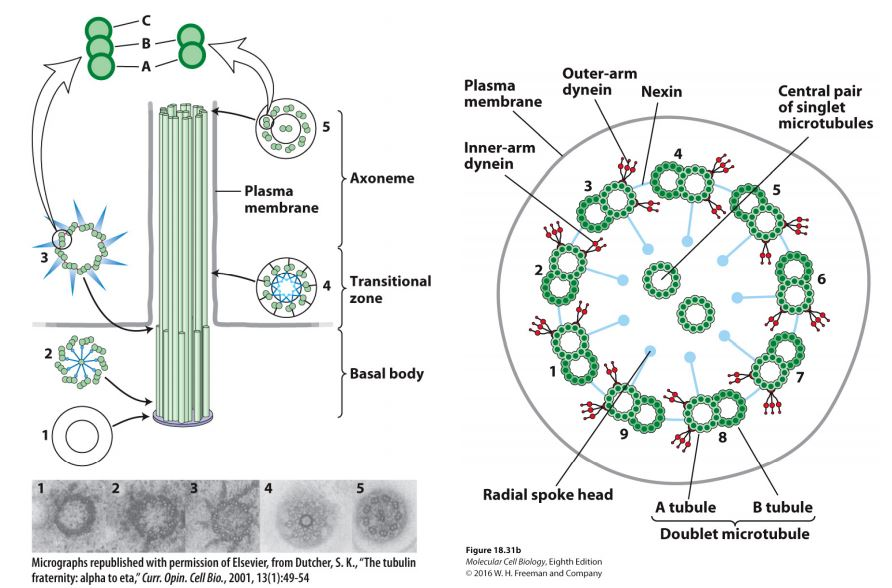
\includegraphics[width=0.6\textwidth]{images/cilia.JPG}
                \caption{\small struttura del cilio o flagello}
                \label{fig:mesh1}
            \end{figure}
        
        \subsubsection{Dineina flagellare}
            I flagelli utilizzano la DIN flagellare, che ha una conformazione differente da quella vista nei paragrafi precedenti. Ha una funzione di movimento del flagelli attraverso attività ATPasica (e non di trasposto).
            Concorre anche al ripiegamento del flagello: la DIN sostiene uno slittamento tra le coppie di MT, la nessina non permette che i due MT scorrano interamente l'uno sull'altro.
            
        \subsubsection{Cilio primario}
            Nel flagello avviene un trasporto attivo di ITF-particles, sostenuto da CHI2 e DIN citoplasmatica, è vitale per la funzione del flagello.
            In moltissime cellule umane/animali esiste il cilio primario che serve come "antenna" per captare segnali provenienti da altre cellule. Ha una struttura differente dal cilio presentato prima, non ha DIN flagellare e non ha i due MT centrali.\\
            La presenza del cilio primario è associata a periodi della vita della cellula in cui è proliferante, viene degradato per permettere al centrosoma di svolgere le funzioni pertinenti alla duplicazione.\\
            Le appendici distali e sub-distali sono necessari per diventare corpuscolo basale, infatti sono necessarie per nucleare i MT del cilio. Difetti nella ciliogenesi causano patologie fenotipicamente e geneticamente molto eterogenee.
    
    \subsection{MT nel ciclo cellulare}
        Il ciclo cellulare si divide in cinque fasi principali: G0, G1, S, G2 e M.\\
        La fase G0 è la fase di vita cellulare non in replicazione. \\
        La fase G1 è la fase in cui viene replicato il materiale cellulare, è presente un solo centrosoma con due centrioli circondati da PCM (peri-cerntiolar material) con $\gamma$T, organizzano MT nello spazio.\\
        La fase S presenta i cromatidi replicati e sono coesi (anello “intrappola” due doppie eliche DNA dei cromatidi fratelli).
        Ogni centriolo genera un pro-centriolo (non maturo), generata da centriolo madre, crescita ortogonale al centriolo madre (mediato da PLK – 4, chinasi).\\
        In fase G2 vi è una doppia quantità DNA, i cromatidi fratelli sono legati da anelli di coesina. Sono presenti 4 centrioli.\\
        La durante la fase M c'è un coinvolgimento più vario dei MT\\	In questa fase avviene la compattazione della cromatina, la trascrizione è sospesa perché dovrà essere separata in due cellule. Ogni centrosoma può liberamente percorrere spazio e formare i due MTOC separati. \\
        Ci sono tre tipi di MT:
        \begin{itemize}
            \item astrali: contatti con cortex e orientamento
            \item polari: interdigitazione, rigidità strutturale
            \item in contatto con cinetocori: contatto con uno dei due cromatidi fratelli
        \end{itemize}
        
        \subsubsection{Profase}
            In profase avvengono i seguenti step:
            \begin{enumerate}
                \item separazione dei due MTOC
                \item riorganizzazione estesa della rete dei MT
                \item condensazione cromosomi
                \item assemblaggio cinetocori
                \item dissoluzione parziale anelli di coesina
            \end{enumerate}
            In particolare la separazione dei centrioli avviene grazie alla CHI-5 che opera lo scorrimento dei MT antiparalleli (allontanamento centrosomi).
            
            L'assemblaggio dei cinetocori (complesso proteico presente sulla porzione centrale del cromosoma in corrispondenza del DNA centromerico) prende luogo perchè possa interagire con i MT. 
            La sua formazione è dovuta a differenza locale nella struttura istonica (CEMP-A al posto di H3, dalla quale dipende la formazione delle altre proteine del cinetocore). Il cinetocore presenta siti per interazione con l’estremità + dei MT.
            
            Infine vengono dissolti gli anelli di coesina ad eccezione che nella zona centromerica (conferendo la tipica forma a X), il quale evento segna la fine della profase.
            \begin{figure}[h]
                \centering
                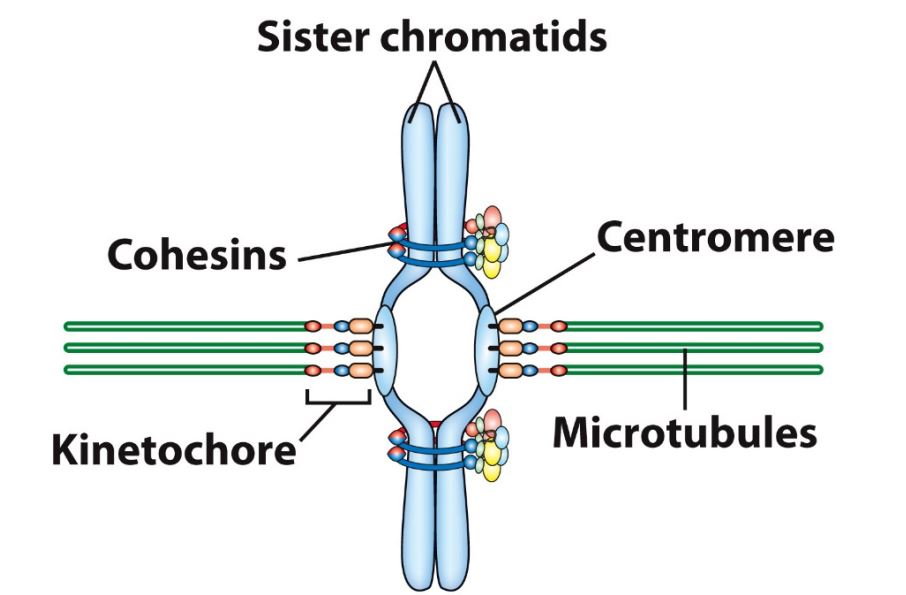
\includegraphics[width=0.5\textwidth]{images/cromatidi.JPG}
                \caption{\small Cromatidi fratelli, cinetocore fornisce ancoraggio a MT}
                \label{fig:mesh1}
            \end{figure}
            
        \subsubsection{Prometafase}
            In prometafase avvengono i seguenti eventi:
            \begin{enumerate}
                \item dissoluzione della membrana nucleare
                \item cattura dei cromosomi da parte dei MT
                \item bi-orientazione e congression
            \end{enumerate}
            Dal momento che cromosomi e MT si trovano nello stesso ambiente (citoplasma) può avvenire l’interazione tra l’estremità + dei MT e il cinetocore.\\
            Di seguito le fasi e le nozioni per sintetizzare bi-orientazione e congression:
            \begin{enumerate}
                \item un cromosoma si dice mono-orientato quando viene agganciato da un MT
                \item si oppongono al movimento netto di un centrosoma mono-orientato verso il centrosoma varie forze (che consistono di molti fattori, es: CHI-4) per arrivare alla bi-orientazione (per congression si intende movimento che prevale)
                \item un cromosoma di dice bi-orientato quando si stabilisce una tensione equilibrata tra i due poli della cellula, quindi quando ogni cromatidio è associato a MT di MTOC diversi
                \item i cromosomi bi-orientati convergono sulla piastra metafasica (anche in tempi diversi)
            \end{enumerate}
            
            \textbf{Regolazione MT e cinetocore con Ndc80 e Aurora B}\\
            \textit{Ndc80 è un complesso (presente in molte copie) la cui formazione innata attorno si MT favorisce l’interazione con il cinetocore. Presenza regolata anche con modifiche post-traduzionali.\\
            Aurora B è una chinesina che fa parte di CPC (Chromosomal Passenger Complex) ed è presente sul centromero. \\
            Si genera una tensione che deforma regioni centrometiche, cinetocore esterno viene orientato verso i poli del fuso per separare i cromatidi promuovendo una defosforilazione di Ncd80 (da parte di Aurora B) e i cinetocori sono più affini ai MT.\\
            L’interazione tra Ncd80 e Aurora B costituisce un metodo per correggere errori (error correction) dovute a tensioni differenti su un cromosoma. Così facendo infatti si destabilizza l’interazione con i MT e la mitosi non può continuare.\\
            \[L'autore non ha capito questa parte\]}
        \subsubsection{Metafase}
            Durante la metafase (definita per esclusione) in cui i cromatidi fratelli sono bi-orientati e sono riusciti a convergere sulla piastra metafasica tenuti in tensione.\\ Avviene l'apertura ultimi anelli di coesina in corrispondenza del centromero.

        \subsubsection{Anafase}
            Durante l'anafase avvengono due eventi in simultaneo: il movimento dei cromatidi verso poli opposti, aumento distanza tra cromatidi (A) e l'aumento distanza interpolare con conseguente elongazione del fuso (B).\\
            La fase A contempla i seguenti step: 
            \begin{enumerate}
                \item depolimerizzazione estremità MT positiva dovuta all’aumento di catastrofi, generazione movimento verso il centrosoma (intervento di CHI-13) grazie all’energia generata dalla depolimerizzazione
                \item depolimerizzazione estremità MT negativa, fenomeno di treadmilling CHI13
            \end{enumerate}
            La fase B sono coinvolte CHI-5 che promuovono lo shift dei MT in posizione centrale (antiparalleli) e una DIN associata a MT corticali avvicina il fuso verso la membrana plasmatica.

        \subsubsection{Telofase}
            Avviene la riformazione involucro nucleare.
            
            \begin{figure}[h]
                \centering
                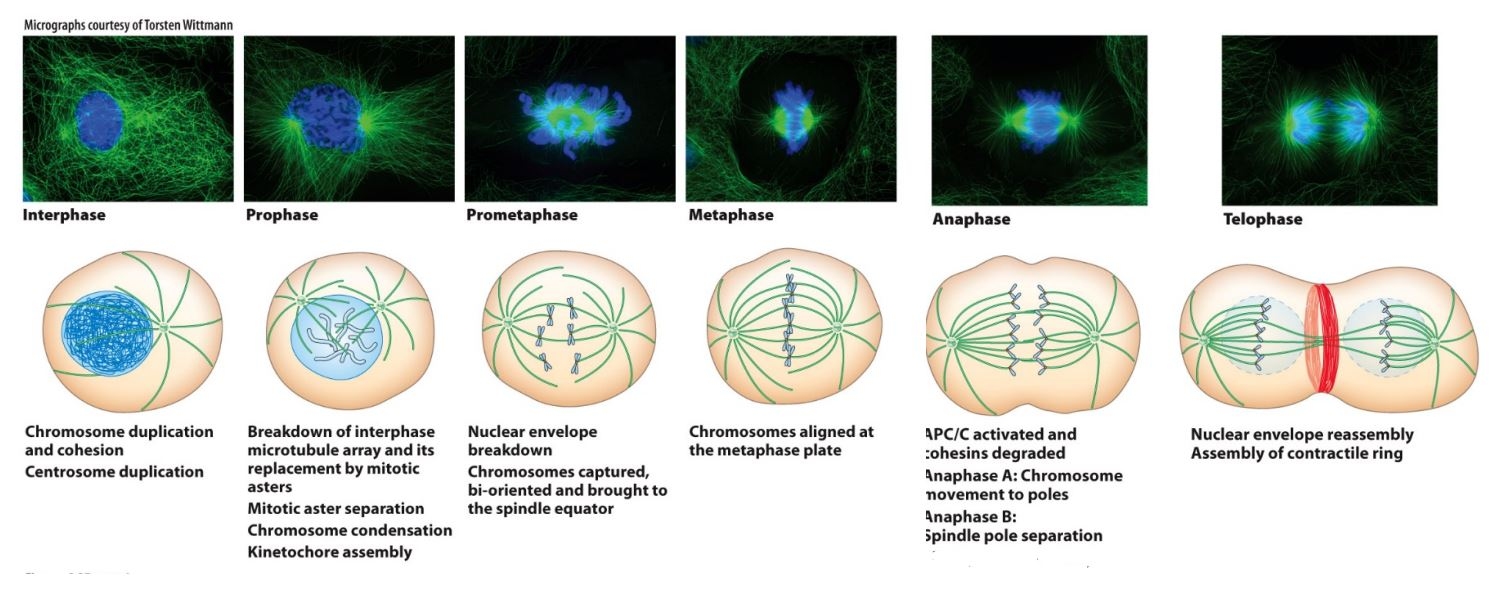
\includegraphics[width=1\textwidth]{images/mitosi.JPG}
                \caption{\small fasi della mitosi}
                \label{fig:mesh1}
            \end{figure}
            
        \subsubsection{Citocinesi e cariochinesi}
            Per citochinesi si intende la separazione fisica a livello citoplasmatico delle due cellule. Non è un processo separato da altre fasi cellulari, ma avviene in simultaneo alle ultime fasi della mitosi, comincia in corrispondenza dell’anafase.\\
            Per cariochinesi si intende la separazione dei nuclei (e corredi genetici), corrispondenti alle prime 5 fasi della meiosi.\\
            
            \textbf{Aurora B e CPC}\\
            In pro/prometa/metafase, Aurora B e CPC sono localizzati al centromero.\\
            Durante anafase si rilocalizzano sulla spindle midzone, hanno affinità con MT antiparalleli e mantengono questa localizzazione anche in telofase.\\
            Si forma un anello contrattile che determina invaginazione (fatto di actina e miosina), che si genera in corrispondenza della posizione di Aurora B (fornisce alla cellula le “coordinate” per la separazione).
            
\section{Filamenti intermedi}
    I FI hanno una composizione eterogenea tessuto-specifica. Hanno un diametro di circa 10 nm.
    Sono presenti anche all'interno del nucleo. Danno rigidità ai tessuti, non hanno polarità intrinseca, non sono legate a nucleotidi fosfati, non sono note proteine motore che interagiscono con FI (correlato al fatto che non hanno polarità) e hanno dinamicità limitata.
    
    \subsection{Struttura}
        70 geni differenti codificano per i FI. Sono dei dimeri paralleli che formano dei coiled coil. I domini C e N terminali sono specifici in base al tessuto e possono essere tra loro molto diversificati. Ogni dimero può associarsi ad un altro dimero in modo antiparallelo.\\
        Un protofilamento è composto da 4 FI associati in maniera antiparallela, 4 protofilamenti formano una \textit{protofibrilla}.
        \begin{figure}[h]
            \centering
            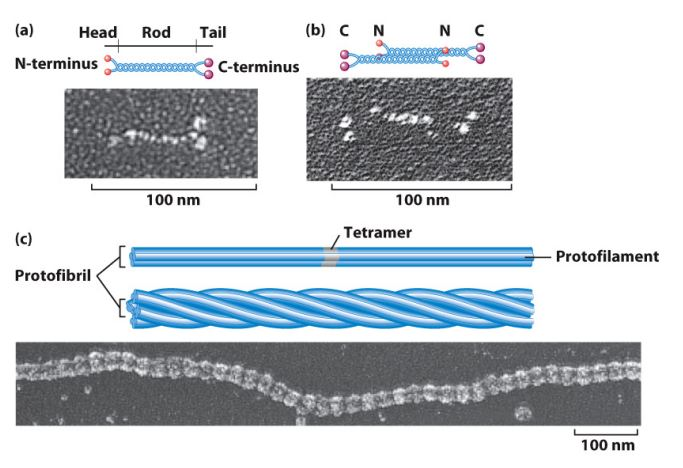
\includegraphics[width=0.7\textwidth]{images/filametiIntermedi.JPG}
            \caption{\small struttura dei FI e della protofibrilla}
            \label{fig:mesh1}
        \end{figure}
    \subsection{Classi}
        I FI si dividono in classi.
        \subsubsection{Cheratina acida e basica}
            Sono due classi differenti (acida e basica) che però collaborano strettamente, sono sempre associate a coppie acida-basica. Sono codificate da 50/70 geni e sono ampiamente presenti a livello epiteliale. Contribuiscono alla rigidità della cellula.
        \subsubsection{Desmina, vimentina e GFAP}
            Sono FI presenti delle cellule muscolari, gliali e mesenchimali. Si occupano dell'organizzazione del sarcomero e hanno funzioni tra loro differenti.
        \subsubsection{Neurofilamenti}
            Sono presenti nelle cellule neuronali e contribuiscono all'organizzazione dell'assone. Si dividono in categorie differenti perchè sono tre tipologie che collaborano (light, heavy e medium).
        \subsubsection{Lamìne}
            Sono FI presenti nel nucleo che contribuiscono alla sua organizzazione e struttura.
            Sono ubiquitari, in assoluto i più comuni. Interagiscono con il cortex per la membrana nucleare. \\
            Le lamìne formano un reticolo sottostante alla membrana nucleare (interna) e si associa alla membrana in modi differenti (tramite proteine o la sua struttura è modificata direttamente per l'interazione). \\
            Interagisce con la cromatina per il suo metabolismo, preferibilmente con regioni eterocromatiche.\\
            La mutazione di questa proteina compromette la stabilità del DNA.\\
            Risulta in continuità con altri elementi citocheletrici citoplasmatici, infatti esistono proteine specifiche che consentono l'interazione della lamìna con MT, FI e MF.\\
            Esistono proteine diverse che sostituiscono la classe delle lamìne [A, B1, B2, C]. Le proteine A e C derivano dallo splicing alternativo dello stesso gene.\\
            In prometafase, la dissoluzione del nucleo avviene anche grazie alla fosforilazione della lamìna (che è un processo reversibile).

\section{Microfilamenti}
    I microfilamenti (detti anche filamenti di actina) sono intimamente legati alla membrana citoplasmatica, sono deputati al movimento della cellula e alla definizione della forma della membrana. In cellule polarizzate definisce il leading edge. I MF determinano la forma della cellula in base ai segnali dei recettori delle membrane: l'actina è la componente citoschelettrica più fortemente condizionata dal signaling. Hanno un diametro di 6/7 nm.\\
    L'actina ha strutture e funzioni diverse:
        \begin{itemize}
            \item microvilli
            \item cortex cellulare
            \item connessione cellule
            \item movimento delle vescicole
            \item formazione lamellipodi e fillopodi
            \item stress fibers (presenti fisiologicamente)
            \item fagocitosi
            \item anello contrattile
        \end{itemize}
    A livello sperimentale viene utilizzata la \textit{falloidina} che lega l'actina e ne permette l'osservazione "immobilizzandola" nel caso di cellule vive.
    
    \subsection{Struttura}
        L'actina è composta da un singolo polipeptide ed è codificata da molteplici geni. Il singolo monomero che compone il filamento di actina (F-ACT) è l'actina globulare (G-ACT) che presenta una tasca per l'associazione con l'ATP.\\
        Il F-ACT è polarizzato (l'estremità positiva non espone la tasca per ATP, quella negativa si), sono necessarie 14 G-ACT per compiere un giro.\\
        La miosina è una proteina che interagisce fortemente con l'actina e che si lega ad essa con un angolo specifico, osservando l'angolo si deduce l'orientamento del F-ACT (si forma una "freccia" che indica l'estremità negativa).
        \begin{figure}[h]
            \centering
            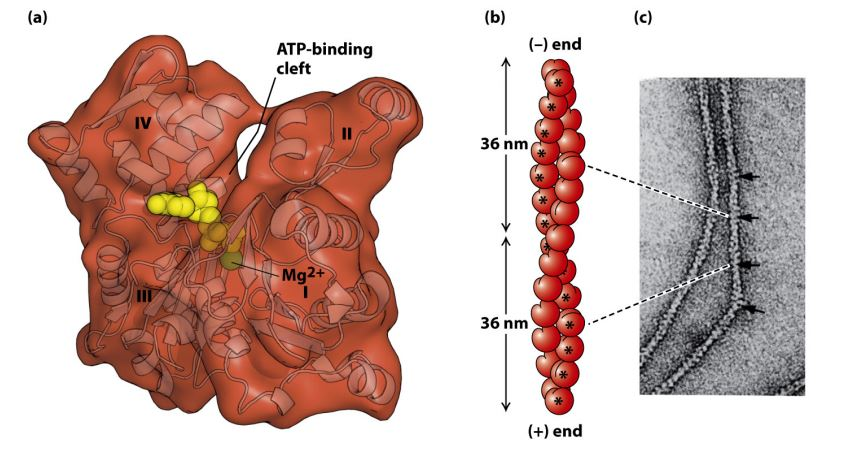
\includegraphics[width=0.7\textwidth]{images/G-ACTeF-ACT.JPG}
            \caption{\small Struttura della actina globulare e del filamento}
            \label{fig:mesh1}
        \end{figure}
        
        \subsubsection{Comportamento dell'actina purificata}
            In vitro si riesce a studiare il comportamento dell'actina purificata per quanto riguarda la sua crescita e decrescita. Si notano tre fasi: lag, elongation e una fase di stallo.
            \begin{enumerate}
                \item LAG: è la fase iniziale a cui si assiste alla formazione di un nucleo di tre G-ACT che costituiscono il seme su cui si baserà l'orientamento e la struttura di tutto il F-ACT.
                \item ELONGATION: una fase di rapida elongazione del filamento
                \item STALLO: equilibrio tra concentrazione di G-ACT e quella presente su F-ACT. Avviene in corrispondenza della concentrazione critica CC.
            \end{enumerate}
            
    \subsection{Dinamica dei MF}
        La dissociazione della G-ACT avviene a prescindere dalla sua concentrazione. L'aggiunta a un F-ACT di G-ACT dipende invece dalla concentrazione, la concentrazione critica dell'estremità positiva differisce da quella all'estremità negativa.
        La G-ACT possiede un'innata propensione ad idrolizzare ATP e rilasciare il fosfato. All'equilibrio il dominio positivo di F-ACT possiede ATP, i domini intermedi ADP+P e quella negativo solo ADP.\\
        L'idrolisi dell'ATP riduce la propensione della G-ACT a rimanere associata a un F-ACT.
        Anche i MF presentano il processo di treadmilling (l'accrescimento all'estremità positiva, depolimerizzazione all'estremità negativa).
        Il treadmilling del preparato di sola actina è è 10 volte pià rapido di quello espresso in vivo.
            
        \subsubsection{Agenti promotori ed inibitori}
            Ci sono degli agenti che ne modificano il comportamento:
            \begin{itemize}
                \item Profilina: lega G-ACT legata a ADP e catalizza lo scambio con ATP, quindi ne velocizza la polimerizzazione.
                \item Cofilina: lega protofilamenti di F-ACT e ADP e ne catalizza la depolimerizzazione all'estremità negativa.
                \item Timosina $\beta$4: lega G-ACT e ATP quando questa è monomerica. In questo modo non può essere incorporata in un F-ACT (si forma una "riserva").
                \item CapZ e Gelsoina: si legano all'estremità positiva e previene l'aggiunta di F-ACT. Promuove la decrescita.
                \item Tropomodulina: si lega all'estremità negativa di F-ACT e ne previene il disassemblaggio. Promuove la crescita.
                \item Formina: è una proteina composta di più domini catalizza l'assemblaggio di F-ACT. Il dominio FH2 stabilisce il contato tra due G-ACT orientate correttamente e possibilmente cambia conformazione man mano che si aggiunge G-ACT. Il dominio FH1 ha affinità per profilina che promuove una crescita locale. Il dominio RBD interagisce con $\rho$GTP, regola il ripiegamento per l'autoinibizione (in assenza di $\rho$GTP) o scatena l'attività della formina in sua presenza.
                Può inibire l'associazione con CapZ rimanendo associata all'estremità positiva.
                \item Complesso ARP (\textit{actin related protein}): consiste di sette subunità, promuove la nucleazione di G-ACT con ramificazione. Utilizza NPF (\textit{nucleation promoting factor}) che predispone la G-ACT spazialmente per la nuova nucleazione di F-ACT. Il ramo cresce inclinato di 70° e sono strutture ricorrenti nei lamellipodi.
                Alcune NPF (per esempio WASp) vengono mantenute inattive finchè non intervengono due segnali contemporaneamente scatenati da input diversi. \\
                L'actina ramificata contribuisce anche alla fagocitosi. Un leucocita incapsula un battere riconosciuto tramite un anticorpo, promossa dalla locale attivazione di ARP 2/3.
                \end{itemize}
                \begin{figure}[h]
                    \centering
                    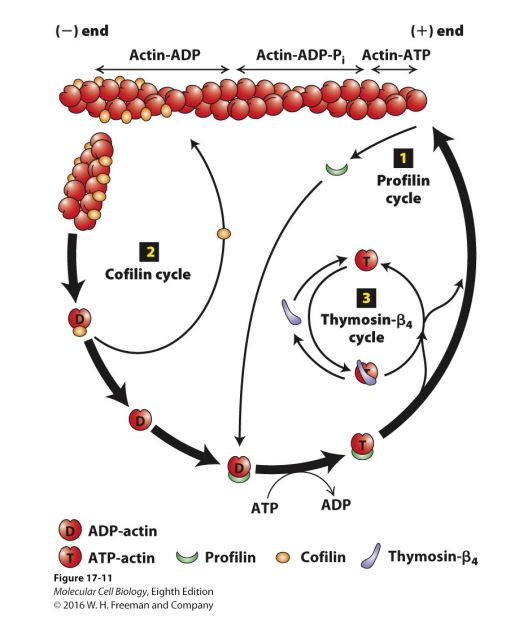
\includegraphics[width=0.7\textwidth]{images/agentiActina.JPG}
                    \caption{\small interazione timosina, profilina e cofilina con il filamento di actina}
                    \label{fig:mesh1}
                \end{figure}
            
        \subsubsection{Strutture particolari con fattori di movimenti}
            Si possono formare strutture di MF più complesse con l'interazione di ACLP (\textit{actine cross linking proteins}) che hanno più siti di legame per l'organizzazione dei filamenti nello spazio. Ricordiamo tra queste $\alpha$actina, fimbrina, spectrina, filamina e distrofina.   \\
            La spectrina è una molecola che organizza i MF in prossimità del cortex con una disposizione a raggera. Funge anche da hub tra proteine di membrana.\\
            La distrofina può essere geneticamente difettosa, in quel caso può causare patologie quali la distrofia muscolare (ma non solo).
            
    \subsection{Miosine}
        Le miosine, sono una famiglia di proteine che funge da motor protein per i MF. Hanno in comune una testa ma la coda è specifica. Il loro movimento deriva dall'idrolisi dell'ATP e assumono molti aspetti specifici (sono codificate da circa 40 geni diversi). Esistono molteplici mutazioni di questi 40 geni che causano patologie anche ereditarie.\\
        In generale camminano verso l'estremità positiva (tranne la miosina 6).
        
        \subsubsection{Miosina 1}
            La MI1 ha a caratteristica di avere una sola catena pesante, il suo passo corrisponde a 10-14 nm, è associata alla membrana e sostiene l'endocitosi. Alcuni membri di MI1 interagiscono direttamente con i lipidi.
            
        \subsubsection{Miosina 5}
            La MI5 ha una \textit{duty rate} di circa il 70\% quindi risulta molto processiva ed è coinvolta nel trasporto di organelli. La porzione della proteina che si pone tra lo stelo e i piedi è più allungata e quindi ha un passo di lunghezza maggiore (passo di 36 nm).\\
            La MI5 è utilizzata nella duplicazione del lievito (\textit{budding yeast}), si forma infatti un F-ACT nella nuova gemma e MI5 trasporta diverse molecole e organelli in direzione della gemma (anche estremità di MT).\\
            Anche nell'uomo è presente la MI5 ma se sue funzioni non sono ben comprese e definite come per il lievito.
            
        \subsubsection{Miosina 6}
            La MI6 è eccezionalmente una miosina che cammina vero l'estremità negativa del filamento di actina.
            
        \subsubsection{Miosina 2}
            La miosina 2 (MI2) è quella storicamente più importante, è ampiamente presente nel muscolo scheletrico e anche nelle cellule muscolari cardiache. Ne esistono circa 20 tipi diversi.    \\
            Esistono 16 geni che le codificano, utilizzano ATP per il lavoro meccanico e sono presenti anche in tessuti non muscolari. Il loro passo compie 8 nm.\\
            
            \textbf{Struttura}\\
            Sono composte da una catena pesante formata da un coiled coil, delle catene leggere regolatrici e leggere essenziali e dei siti attivi. Le ultime tre componenti insieme (porzione S1) lega direttamente l'actina e il nucleotide tri-fosfato. Migra verso il polo positivo dell'actina.\\
            \begin{figure}[h]
                \centering
                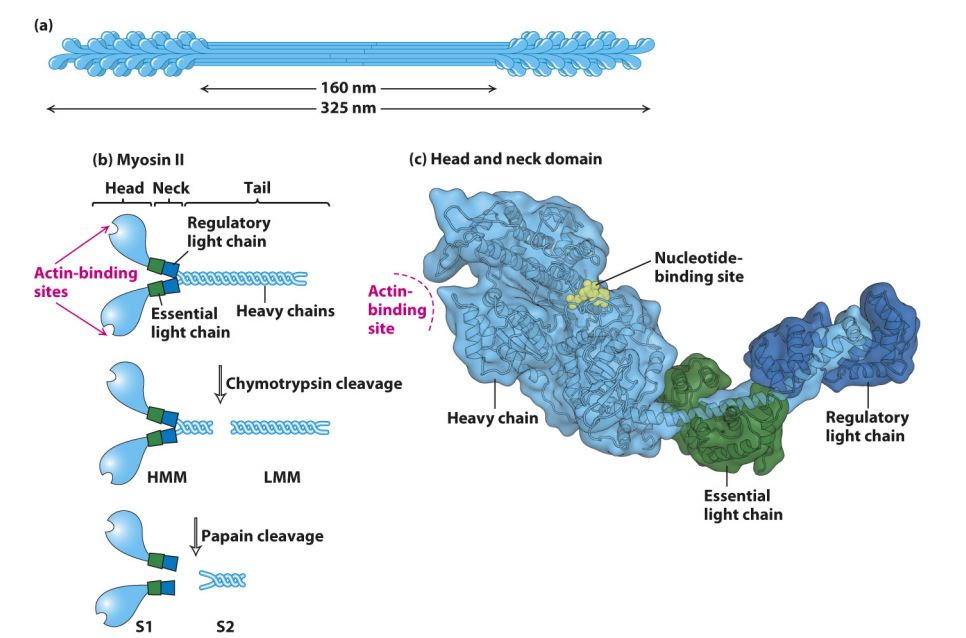
\includegraphics[width=0.7\textwidth]{images/miosina.JPG}
                \caption{\small Struttura della miosina2}
                \label{fig:mesh1}
            \end{figure}
            
            \textbf{Cammino}\\
                Il movimento della MI2 è possibile grazie all'idrolisi di ATP e il suo passo è di 8nm. 
                In particolare avviene secondo questi step:
                \begin{enumerate}
                    \item legame al MF saldo, MI2 non è legata ad ATP
                    \item rilascio della testa e legame con ATP
                    \item idrolisi dell'ATP causa un movimento del dominio
                    \item nuovo contatto con MF e rilascio dell'ADP per saldarsi all'actina
                \end{enumerate}
                Alterando la lunghezza del collo della MI si ottiene una velocità differente (proporzionale all'allungamento del passo). \\
                Per \textit{duty rate} si intende la percentuale di tempo che la testa passa legata al MF. Questo periodo dipende dalla propensione a rilasciare ADP. La duty rate di MI5 è maggiore di MI2. \\
            
            \textbf{Regolazione contrazione}\\
                Le cellule muscolari si assemblano in strutture superiori chiamate \textit{sincizi}. Queste consistono in cellule plurinucleate e si organizzano in fasci. I sincizi vano a loro volta a formare le miofibrille, la cui contrazione è regolata dal sarcomero: un assemblamento di ACT e MI. \\
                Nel sarcomero sono presenti anche altri agenti, in parte già visti in precedenza, quali:
                \begin{itemize}
                    \item titina: in continuità tra ACT e MI
                    \item nebulina: determina la lunghezza dell'ACT
                    \item tropomodulina, troponina e tropomiosina
                    \item CapZ
                \end{itemize}
                La contrazione viene regolata in dipendenza da ioni calcio $Ca^{++}$.
                \begin{enumerate}
                    \item arriva un segnale nervoso che rilascia ioni $Ca^{++}$ dal reticolo sarcoplasmatico. 
                    \item aumento della concentrazione di $Ca^{++}$ citoplasmatica
                    \item $Ca^{++}$ lega una subunità della troponina (a sua volta legata alla tropomiosina) associata ai F-ACT
                    \item spostamento della tropomiosina, esposizione dei siti di legame con la MI prima mascherati
                    \item contatto MI2 e F-ACT che determinano la possibilità di entrare nel ciclo di contrazione
                \end{enumerate}
                \begin{figure}[h]
                    \centering 
                    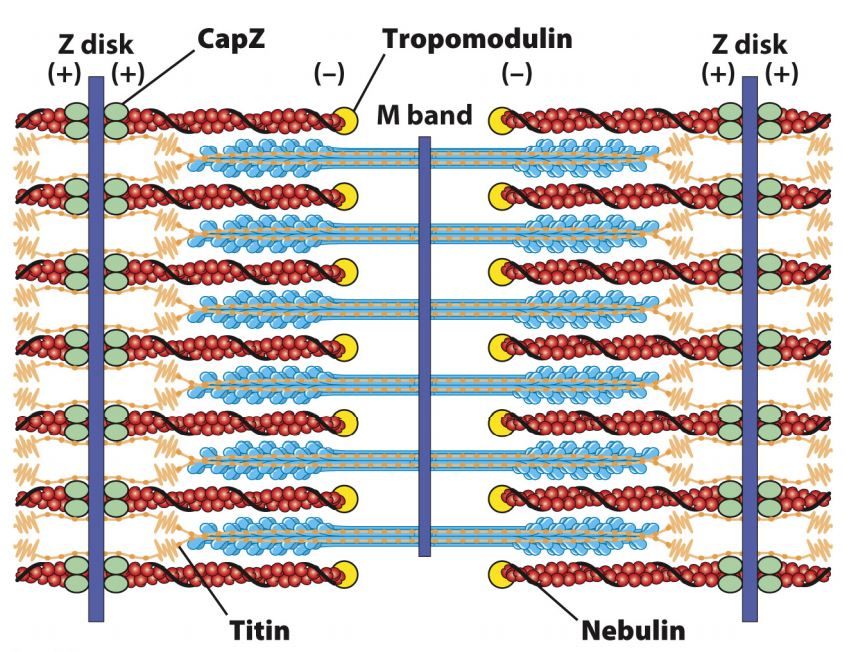
\includegraphics[width=0.5\textwidth]{images/sarcomero.JPG}
                    \caption{\small Struttura del sarcomero}
                    \label{fig:mesh1}
                \end{figure}
            
            \textbf{Contrazione nel tessuto muscolare liscio}\\
                Il tessuto muscolare liscio non presenta sarcomeri, la sua contrazione avviene senza l'interazione tra ACT e MI.
                La contrazione avviene per un meccanismo di fosforilazione e defosforilazione di una proteina target, ovvero la catena leggera regolatoria.\\
                ATP cede il suo P alla proteina target che forma un legame covalente. Il bilancio energetico è favorevole. Questo evento cambia la conformazione della proteina target che ne modifica l'attività.
                A seconda della proteina target, può essere la defosforilazione che determina il suo attivamento.\\
                \textbf{Gli AA che tipicamente possono essere fosforilati sono serina, treonina e tirosina}. La fosforilazione viene tipicamente promossa da una protein-chinasi per serina e treonina o tirosina (due gruppi di protein-chinasi) o da una protein-fosfatasi.\\
                La MI2 può essere regolata dalla fosforilazione della catena leggera che quindi regola l'esposizione del Coiled coil e la contrazione. Protein chinasi e fosfatasi collaborano per la contrazione. In particolare avvengono questi step:
                \begin{enumerate}
                    \item $Ca^{++}$ provoca un segnale
                    \item $Ca^{++}$ lega la CAM (calmodulina) e attiva MLC-chinasi
                    \item contrazione
                \end{enumerate}
                Il meccanismo regolato in questo modo risulta molto più lento perchè $Ca{++}$ deve diffondere nella cellula senza sarcoplasma.\\
                
            \textbf{Altre funzioni di MI2}\\
                La MI2 è impiegata anche per la formazione dell'anello contrattile (assieme all'ACT) durante anafase e telofase per la citochinesi. \\
                Assieme all'ACT, MI2 ha un ruolo fondamentale per la formazione di anelli contrattili a livello apicale delle cellule epiteliali.\\
                
            \textbf{Tossine}\\
                Esistono varie tossine che alterano il comportamento della MI2, quali:
                \begin{enumerate}
                    \item citocalesina B e D, che impedisce la polimerizzazione di ACT legandosi all'estremità positiva
                    \item latrunculin che impedisce la polimerizzazione legando la G-ACT
                    \item falloidina che previene la depolimerizzazione, quindi ne impedisce la dinamicità
                \end{enumerate}
            
    \subsection{Migrazione cellulare}
        La coordinazione tra ACT e MI, assieme al livello di concentrazione di $\rho$GTPasi determina gli eventi di locomozione della cellula. Distinguiamo le seguenti strutture e attività della cellula:
        \begin{itemize}
            \item lamellipodio: è l'estensione dell'estremità frontale sostenuta dal treadmilling di ACT ed è regolato da ARP2-3, formazione di ramificazioni di ACT
            \item adesione alla matrice extracellulare ad opera di strutture di adesione focale (mediate da integrine,\textit{ focal adesion}), consente contatto tra citoscheletro interno e matrice extracellulare
            \item traslocazione: lavoro di contrazione di ACT su MI2 interni alla cellula sull'estremità opposto del "senso di marcia"
            \item endocitosi: fase di de-adesione, la nuova membrana che viene utilizzata al leading edge deve essere rigenerata, quindi avviene un riciclo di lipidi di membrana distanti
        \end{itemize}
        
        A livello molecolare, le focal adesion interagiscono con proteine trans-membrana (integrine) che hanno funzioni meccaniche e di signaling per il citoscheletro (oltre che essere ancoraggio fisico). \\
        Le stress fibers sono formazioni di fibre contrattili ACT e MI2 che richiamano l'estremità arretrata.
        
        \subsubsection{Regolazione da cascate di trasduzione del segnale}
            La locomozione cellulare è un esempio di come una cascata di trasduzione di segnali anche extracellulari possano concorrere alla modifica conformazionale della cellula.\\
            La cascata di signaling è operata dalla famiglia di proteine $\rho$, sono GTPasi globulari con ancora lipidica associata alla membrana (foglietto citosolico), possono associarsi a GTP o GDP e in base a questi generano segnale (con GTP interagiscono con proteine effettrici che veicolano segnali a valle). Associata al GDP abbiamo la conformazione inattiva.\\
            Quando $\rho$ è esposta nella membrana interagisce con
            \begin{itemize}
                \item GEF (promozione scambio GDP con GTP) che ne induce attivazione
                \item GAP (promozione idrolisi GTP) che ripristina uno stato inattivo.
            \end{itemize}
            \begin{figure}[h]
                \centering
                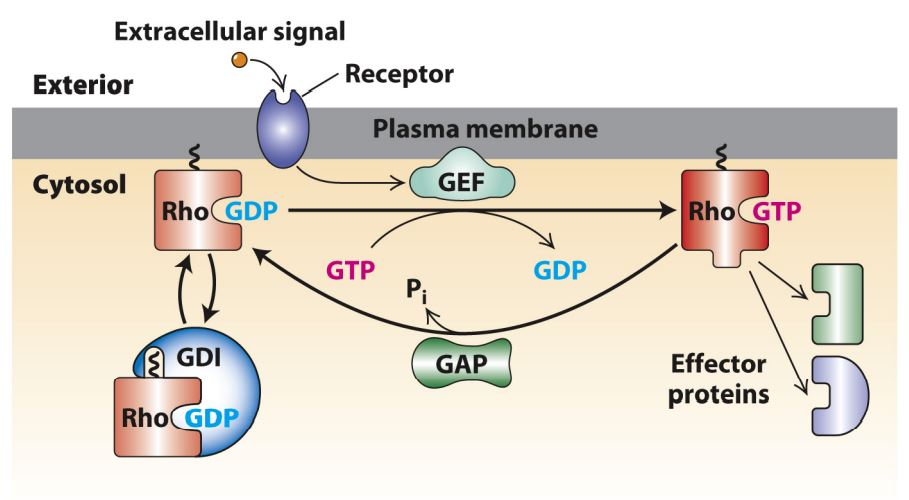
\includegraphics[width=0.5\textwidth]{images/RhoGEFeGAP.JPG}
                \caption{\small Interazione di $\rho$ con GEF e GAP}
                \label{fig:mesh1}
            \end{figure}
            
            \textit{
                \textbf{Dominanza negativa}\\
                Per dominanza negativa si intende una mutazione che influenza negativamente di un gene wild type (wt), può essere una versione di un gene mutata che compromette il corretto funzionamento possibilmente anche di altri complessi. Per le $\rho$GTPasi potrebbe essere una proteina che modifica interazione con GEF.\\}
            
            \textit{    
                \textbf{Dominanza positiva} \\
                Per dominanza positiva si intende un gene mutante che impedisce l'inattivazione di altri complessi. Nel caso delle $\rho$GTPasi, la modifica di un singolo AA muta il legame costitutivo con GTP per esprimere segnali.}\\
            
            Se esprimo nella stessa cellula diversi dominanti attivi di tre diverse $\rho$GTPasi osservo in ogni caso un rimodellamento del citoscheletro di ACT (ognuna singolarmente):
            \begin{itemize}
                \item $\rho$ dominant active determina formazione eccessiva di stress fibers
                \item CDC dominant active determina fillopodi in ogni direzione
                \item RAC dominant active determina la formazione di membrane ruffles
            \end{itemize}
            Un approccio readout molto comune è lo \textit{scretch essay} in cui cresco delle cellule sulla petri, esercito una discontinuità e dopo una certa quantità di tempo le cellule migrano e tornano ad occupare lo spazio dello scatch. 
            I tre dominanti positivi sopra rallentano il processo migratorio di questo esperimento. \\
            Al leading edge, il treadmilling è iniziato e promosso da attivazione di CDC42 (selettivamente alle porzione di membrana frontale al movimento) che determina l'attivazione di RAC (al leading edge) che che interagisce con ARP23 che causa il treadmilling. Al contempo, RAC determina l'attivazione di $\rho$ nella porzione distante della cellula che induce la contrazione dei filamenti di ACT-MI.
            L'interazione inibitoria tra $\rho$ e RAC è importante per compartimentalizzare i comportamenti in porzioni differenti della cellula. Entrambi i processi sono iniziati da CDC42.

\pagebreak
\setcounter{section}{0}

\large{\addcontentsline{toc}{part}{Capitolo 7: Proteine di membrana destinate a organelli differenti}}
\Huge\textbf{Capitolo 7: \\Proteine di membrana destinate a organelli differenti}\\

\small
In generale, la conformazione di una proteina influisce sulla sua destinazione, quindi si basa sulla composizione AA. In un preciso stratch di AA si racchiude la chiave per il target (solitamente all'N terminale), ogni organello ha recettori specifici per la propria sequenza terminale e dei traslocatori per la destinazione. 
Talvolta la targeting sequence è rimossa, ha \textbf{determinata natura chimicha, specifici recettori, specifici canali traslocatori e consuma una determinata fonte di energia.}

\section{Regolazione delle proteine}
    A prescindere dal compartimento cellulare, le proteine possono essere modificate chimicamente per ottenere un comportamento differente. 
    \subsection{Fosforilazione}
        Per fosforilazione di intende l'aggiunta di un gruppo fosfato alla proteina target in corrispondenza di un gruppo ossidrile, tramite una reazione di condensazione. Generalmente sono serina, tisorina e treonina che subiscono questa modifica. \\
        Può avvenire in qualunque compartimento cellulare.
        
    \subsection{Allosteria}
        Per allosteria si intende l'utilizzo di un ligando allosterico che si associa alla proteina in un particolare sito. Questo determina un cambiamento conformazionale di un sito A che determina l'attivazione di un sito B.\\
        Esempi di questa modalità di attivazione sono la Calmodulina tramite lo ione $Ca^{++}$ oppure RAN assieme a GTP e GDP.
        
    \subsection{Ubiquitinazione}
        Per ubiquitinazione si intende l'associazione di ubiquitina (UB) (generalmente catene) per la regolazione dell'emivita della proteina target. Il legame con la catena di ubiquitine determina l'associazione con il proteasoma. \\
        L'UB è una piccola molecola proteica (di soli 76 AA di cui 7 lisine) che risulta estremamente conservata tra speci differenti. Viene utilizzata come marker per la morte di una molecola proteica.\\
            
        L'ubiquitinazione avviene attraverso l'utilizzo di diversi enzimi:
        \begin{enumerate}
            \item E1 (enzima di attivazione dell'UB) che si associa covalentemente a una cisteina dell'UB
            \item E2 (enzima per la coniugazione dell'UB) che forma un legame covalente con una cisteina dell'UB (funzione simile ad E1)
            \item E3 (enzima ligasi per l'UB) che viene promossa dalla presenza di E2 che predispone il substrato proteico per il legame tra esso e l'UB
            \item E4 (non essenziale) che allunga le catene di UB pre-esistenti.
        \end{enumerate}
        Esistono 2 geni per E1, 35 per E2 e più di 100 per E3, questo per aumentare la specificità a substrati diversi. In particolare esistono HECT e RING (due tipologie di E3) che sostengono rispettivamente un legame covalente o un trasferimento diretto. \\
        
        La poliubiquitinazione ha come scopo l'associazione al proteasoma, una macromolecola in grado di degradare la proteina in monomeri o dimeri di AA. Il proteasoma ha dei recettori per UB (lega catene di UB), contiene DUB (de-ubiquitinazione, dissociazione da UB), AAA-ATPasi per svolgere il polipeptide da degradare.\\
        L'aggiunta di UB può avvenire in maniere diverse che assumono scopi differenti, ubiquitinazioni differenti dalla proteina hanno funzioni tuttora ignote e possibilmente molto differenti:
        \begin{itemize}
            \item Poli-UB: segnala la morte della proteina e l'intervento del proteasoma
            \item Multi-UB: UB non forma una catena ma è associata a siti differenti
            \item Mono-UB
            \item Poli-UB ramificate: formazione di ramificazioni di UB tramite legami isopeptidici tra il C-terminale di un UB e una catena laterale di un'altra UB che funge da substrato.\\
            A seconda della lisina coinvolta nell'UB (sono 7 in totale) del substrato assume comportamenti differenti: 
                \begin{itemize}
                    \item Lisina 48: degradazione con proteasoma
                    \item Lisina 63: signaling immunitario
                    \item Lisina 33: controllo linfociti
                    \item Lisina 11: divisione cellulare
                \end{itemize}
        \end{itemize}

\section{Destinazione: RE}
    La sintesi proteica avviene al livello di citoplasma, possibilmente attraverso i ribosomi associati alla membrana del RE. 
    Dopo un'adeguata procedura, si riescono ad ottenere sperimentalmente i mircosomi, ovvero delle vescicole originate dal RE con ribosomi associati utili al fine di studi specifici.
    
    \subsection{Sequenza di targeting}
            Le sequenze di targeting (TS) sono specifiche sequenze di 16-30 AA poste all'N-terminale. Contiene sempre 1 o 2 AA carichi positivamente adiacenti ad uno stretch idrofobico di 6-12 AA. Gli AA idrofobici sono essenziali per la sequenza di targeting.
            Solitamente viene rimossa una volta che la proteina raggiunge il lumen. \\
            Effettuando un esperimento con dei microsomi, si osserva che l'importazione della proteina nel lumen avviene co-traduzionalmente, in particolare la traslocazione avviene entro la traduzione dei primi 70 AA. La TS è compresa nei primi 40 AA quindi risulta già esposta alle proteine traslocanti.\\
            
            \subsubsection{SRP}
                La SRP (\textit{signal recognition particle}) è una ribonucleoproteina che è composta di 6 polipeptidi e un RNA di circa 300 nucleotidi. P54, uno degli esameri che la compongono, interagisce con le TS grazie al suo canale che favorisce l'associazione con la porzione idrofobica.\\
                Un dominio differente lega invece un GTP che promuove l'associazione con un recettore di SRP, una proteina integrale di membrana presente sulla porzione citosolica.
            
            \subsubsection{Importazione}
                \begin{enumerate}
                    \item Il ribosoma sintetizza la prima porzione proteica
                    \item SRP allaccia la porzione idrofobica di TS e la stabilizza
                    \item SRP stabilisce interazioni con i recettori SRP nel momento in cui entrambi sono legati a GTP (specificità)
                    \item avviene l'idrolisi del GTP promossa su entrambi nel momento in cui il complesso è ormai formato che determina l'apertura del canale proteico (il traslocone).
                    \item la TS viene associata al traslocone e avviene il rilascio di SRP
                    \item il neo-polipeptide viene sintetizzato attivamente e grazie all'aumento di AA viene spinto attraverso il traslocone
                    \item la TS viene rimossa
                    \item nel momento il cui il ribosoma incontra il codone di stop si ferma la polimerizzazione, viene rilasciato il traslocone e avviene il rilascio della proteina.
                \end{enumerate}
                \begin{figure}[h]
                    \centering
                    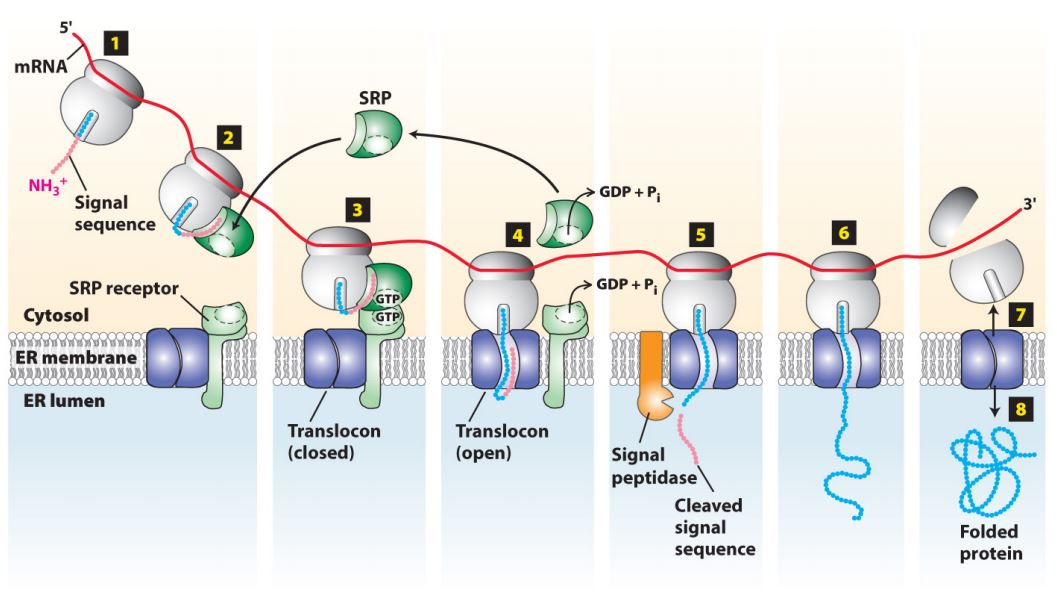
\includegraphics[width=0.7\textwidth]{images/importazioneRE.JPG}
                    \caption{\small Step dell'importazione di una proteina che presenta TS nel RE}
                    \label{fig:mesh1}
                \end{figure}
        
    \subsection{Trasloconi e canali}
        Il traslocone dedito al passaggio dei polipeptidi citato sopra è chiamato SEC61$\alpha$. Presenta una struttura a forma di poro "ristretto" con $\alpha$E di leucina che entrano a contatto con il polipeptide da traslocare.
        Assume la capacità di dilatarsi nel momento in cui viene a contatto con il polipeptide (gating, è presente una componente "plug" che libera ed ostruisce il canale). \\
        SEC63 insieme a SEC61$\alpha$ è un altro meccanismo di traslocazione ma avviene a livello post-traduzionale. Non vi è il coinvolgimento di SRP.
        Viene sostenuto da componenti accessorie che promuovono l'associazione di particoalri proteine (BiP, una chaperon) che lega e idrolizza ATP e in seguito cambia conformazione e diventa prono a legare un polipeptide.  \\
        Risulta quindi possibile traslocare porzioni proteiche a livello post-traduzionale, il principio di funzionamento è molto differente: non è l'energia dell'ATP della traduzione a promuovere la traslocazione, ma sono molteplici molecole di BiP che associate ad una sistematica idrolisi favoriscono l'import dal punto di vista energetico. 
        Una volta traslocata BiP si dissocia e la proteina può assumere la sua conformazione.
        \begin{figure}[h]
            \centering
            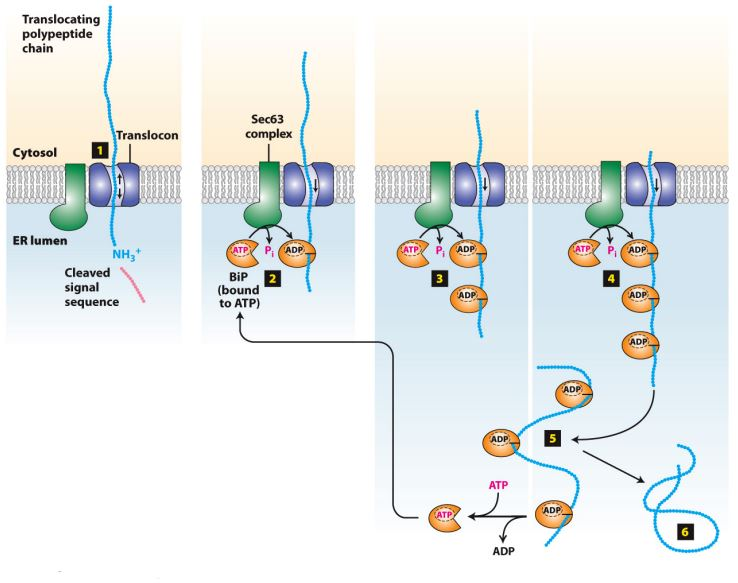
\includegraphics[width=0.7\textwidth]{images/importazioneSEC63-61.JPG}
            \caption{\small Step dell'importazione di una proteina a livello post-traduzionale grazie a SEC61 e SEC63}
            \label{fig:mesh1}
        \end{figure}
        
    \subsection{Sequenze di targeting e inserimento}
        Esistono molte tipologie di proteine transmembrana che dipendono dalle loro sequenze topogeniche, dalla loro posizione e dal loro orientamento. 
        \subsubsection{Sequenze topogeniche}
            \begin{itemize}
                \item \textbf{TS} all'N-terminale
                \item \textbf{STA}, stop transfer anchor interna alla sequenza
                \item \textbf{SA}, anchor signal, simile alla sequenza TS, presenta allo stesso modo una porzione di AA in prossimità dello stretch idrofobico ma è interna alla sequenza AA
            \end{itemize}
            Di seguito le tipologie di proteine transmembrana in base alle loro sequenze topogeniche.
        
        \subsubsection{Tipo 1}
            \begin{figure}[h]
                \centering
                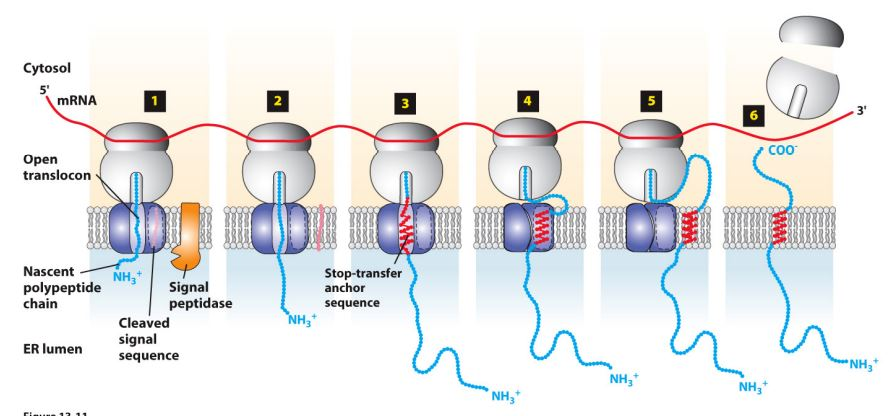
\includegraphics[width=0.7\textwidth]{images/Tipo1.JPG}
                \caption{\small Ancoraggio alla membrana delle proteine di tipo 1}
                \label{fig:mesh1}
            \end{figure}
            Sono polipeptidi con una sequenza topogenica di tipo TS e una STA.\\
            Sono composte da una singola $\alpha$E transmembrana. \\
            \begin{enumerate}
                \item La traduzione inizia da TS all'N-terminale
                \item Produzione di uno stretch altamente idrofobico.
                \item Traduzione della STA
                \item STA raggiunge il traslocone che cambia conformazione in corrispondenza con STA e lascia diffondere lateralmente l'ancora proteica nella membrana
                \item il ribosoma rimane associato fino al codone di stop e poi si dissocia
            \end{enumerate}
            
        \subsubsection{Tipo 2 e 3}
            \begin{figure}[h]
                \centering
                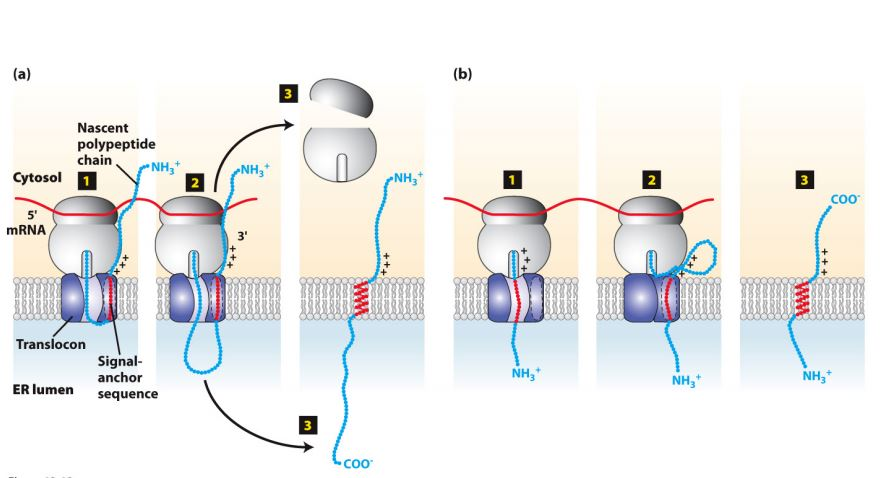
\includegraphics[width=0.7\textwidth]{images/Tipo23.JPG}
                \caption{\small Ancoraggio alla membrana delle proteine di tipo 2 e 3}
                \label{fig:mesh1}
            \end{figure}
            Sono polipeptidi con un singolo SA. \\
            Sono composte da una singola $\alpha$E transmembrana. 
            \begin{enumerate}
                \item Inizio della traduzione della proteina, compresa la porzione contenente AS
                \item SRP riconosce SA e inizia la traslocazione a valle
                \item il ribosoma incontra il codone di stop e si dissocia
            \end{enumerate}
            La differenza tra tipo 2 e tipo 3 sta nella posizione della porzione di AA positivi in relazione allo stretch SA. Per una proteina di tipo 2 sono presenti gli AA positivi precedenti a AS, per quelle di tipo 3 sono posti successivamente.
            Questa piccola differenza fa sì che le proteine di tipo 2 rivolgano il proprio N-terminale a livello del citosol mentre quelle di tipo 3 rivolgano il proprio C-terminale sul lumen.
        
        \subsubsection{Tail Anchor Protein}
            \begin{figure}[h]
                \centering
                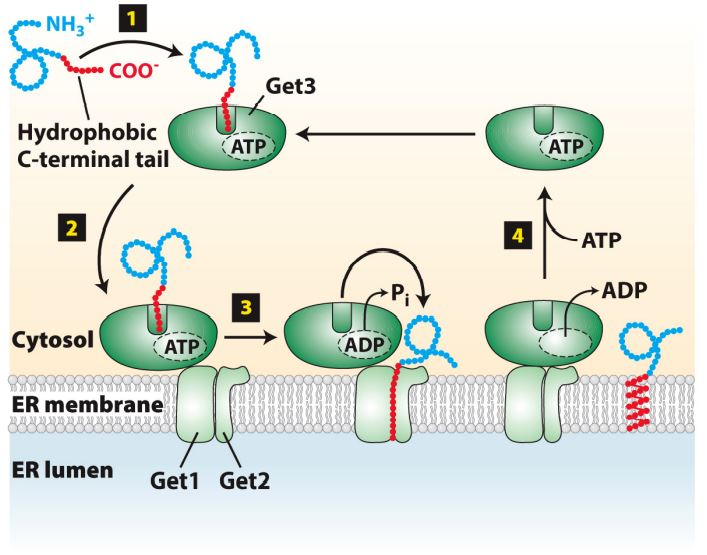
\includegraphics[width=0.5\textwidth]{images/TailAnchrProt.JPG}
                \caption{\small Ancoraggio alla membrana delle proteine di tipo tail anchor protein}
                \label{fig:mesh1}
            \end{figure}
            Sono polipeptidi contenenti una STA.\\
            Sono composte da una singola $\alpha$E transmembrana ma non hanno porzioni che si espongono sul lumen o sulla porzione esoplasmatica.\\
            Non sono coinvolti nè SRP nè il suo recettore, nè il traslocone.
            \begin{enumerate}
                \item La STA è posta al C-terminale, quindi la proteina è ormai interamente tradotta nel momento in cui appare STA
                \item STA viene riconosciuta da Get3 (presente nel citosol) che la protegge finchè non avviene l'interazione con Get1 e Get2
                \item Associazione con Get1 e Get2, idrolisi
                \item Passaggio per un traslocone dedicato
                \item apertura laterale del traslocone e inserimento STA nella membrana.
            \end{enumerate}
            
        \subsubsection{Tipo 4: multipass}
            Sono polipeptidi composti da diverse combinazioni delle classi precedenti. Sono presenti più stretch transmembrana e è possibile qualunque combinazione di N-terminali o C-terminali esposti sul lumen o sul citosol.\\
            Si possono distinguere le classi A e B (vedi figura).
            
        \subsubsection{GPI Anchor Protein}
            Sono polipeptidi contenenti una TS e una STA.\\
            Si associano ad un'ancora lipidica (GPI, \textit{glicosil fosfatidil inositolo}, un lipide con due catene idrofobe e una testa polare), hanno un dominio globulare al C-terminale a livello del lumen-esoplasmatico.
            \begin{enumerate}
                \item GPI è pre-esistente ed è già ancorato alla membrana.
                \item La proteina viene tradotta e traslocata come avviene per quelle di tipo 1. La traduzione viene ultimata prima del contatto con il GPI
                \item la proteina si associa al lipide attraverso l'enzima transamidasi (una sequenza di AA in prossimità a STA viene riconosciuta)
                \item STA rimane come prodotto di scarto
            \end{enumerate}
            Questa tipologia di proteine risulta dispendiosa a livello energetico. \\
            Vengono tuttavia sintetizzate perchè consente alle proteine di membrana di diffondere molto più rapidamente (grazie alla componente lipidica ancorata ad un singolo strato). In cellule con epiteli polarizzati, questa tipologia di ancora rappresenta un segnale per confinare una proteina ad un determinato dominio di membrana.
            \begin{figure}[h]
                \centering
                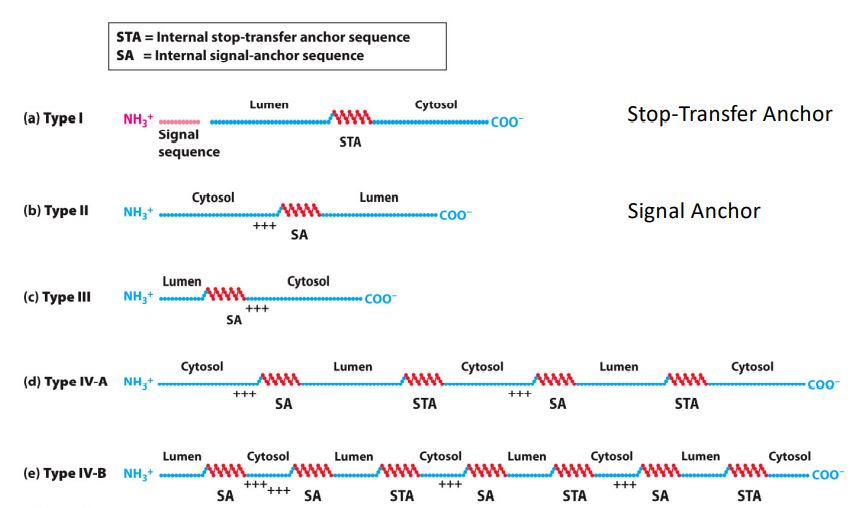
\includegraphics[width=0.7\textwidth]{images/sequenzeTopogeniche.JPG}
                \caption{\small Differenze dello stretch AA delle varie classi di proteine associate alla membrana}
                \label{fig:mesh1}
            \end{figure}
\pagebreak
            
\section{Destinazione: Nucleo}
    Le proteine che hanno accesso al nucleo sono già conformate tridimensionalmente. Passano attraverso il poro nucleare, che è il punto di discontinuità tra le due membrane nucleari quindi il punto di accesso.
    \subsection{Poro nucleare}
        Il poro nucleare (\textit{nuclear pore complex, NPC}) è un conglomerato proteico (16 volte più grande del ribosoma) formato da 30 polipeptidi differenti, le nucleoporine (NAP), ognuno dei quali presente in più copie.\\
        Il NPC è poco selettivo, permette
        \begin{itemize}
            \item la diffusione di piccole molecole
            \item la diffusione di proteine conformate tridimensionalmente fino a 40 KDalton
            \item il traspoto attivo di speci chimiche differenti, quali subunità ribosomiali, mRNA e tRNA
        \end{itemize}
        L'importazione e l'esportazione dal nucleo avvengono molto velocemente.
        \subsubsection{Struttura}
            Il NPC è formato da numerose proteine, tra le quali:
            \begin{itemize}
                \item membrane nucleo-porins: proteine transmembrana, si posizionano sul ripiegamento  che congiunge le due membrane. Vengono organizzate grazie a proteine strutturali
                \item proteine strutturali: organizzano la forma e la struttura del NPC. Ne fa parte il Y-complex, presente ripetuto per 8 volte su entrambe le facce del poro.
                \item FG nucleoporine: nucleoporine ricche di FG (AA fenilalanina e glicina) non strutturate con stretch idrofilici
                \item basket: una struttura di coiled coil sulla porzione interna della membrana
                \item filamenti citosolici: coiled coil che danno sulla parte esterna della membrana
            \end{itemize}
            Il core della struttura del NPC è la matrice di nucleoporine FG, che formano un canale idrogel. 
            \begin{figure}[h]
                \centering
                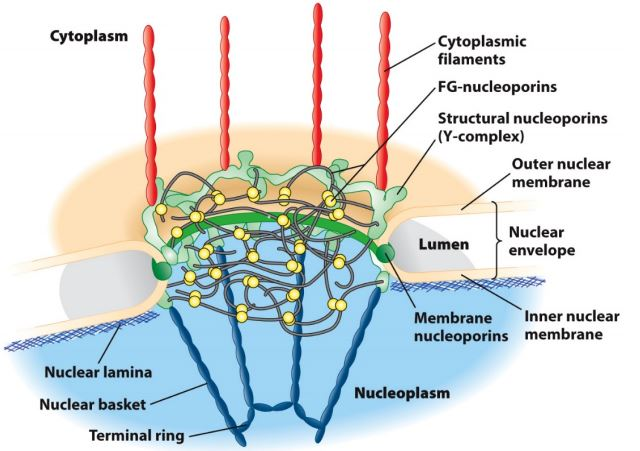
\includegraphics[width=0.7\textwidth]{images/poroNucleare.JPG}
                \caption{\small Struttura di un poro nucleare}
                \label{fig:mesh1}
            \end{figure}
        
    \subsection{Importazione}
        \subsubsection{Nuclear Localization Signal}
            NLS sta per \textit{nuclear localization signal}. L'importazione di una proteina nel nucleo è segnata dalla presenza di una sequenza di AA particolare: 7 AA di cui prolina, lisina e arginina le più presenti, per questo motivo hanno una carica positiva. \\
            Questa sequenza sta generalmente in prossimità del C-terminale e \textbf{non} viene rimossa.
            
        \subsubsection{Processo importazione}
            I fattori coinvolti nell'importazione di proteine nel nucleo sono:
            \begin{itemize}
                \item un recettore di trasporto nucleare, l'\textit{importina}
                \item una RAN (GTPasi, \textit{RAs-related Nuclear protein}), associata a GTP diventa prona ad associazione con importina, associata a GDP non ha affinità
                \item GAP e GEF
            \end{itemize}
            L'importazione segue gli step:
            \begin{enumerate}
                \item L'importina riconosce la sequenza NLS
                \item Il complesso importina-proteina attraversa il NPC grazie alle caratteristiche chimiche dell'importina stessa
                \item RAN (può diffondere attraverso il NPC) si associa a un GTP grazie ad una GEF (pre-esistente nel nucleo) che favorisce l'associazione all'importina e promuove il rilascio del cargo.
                \item RAN-GTP associata ad importina attraversa NPC
                \item una GAP (nel citoplasma) idrolizza il GTP di RAN a GDP, quindi abbiamo la dissociazione tra RAN e l'importina.
            \end{enumerate}
            La GEF nel nucleo e la GAP nel citoplasma mediano l'attivazione e l'inattivazione di RAN (tramite inclusione di GTP o idrolisi a GDP) che entra ed esce dal nucleo per esportare importina, con il fine di poterla riutilizzare.\\
            Per ogni ciclo di RAN si consuma un GTP.
            \begin{figure}[h]
                \centering
                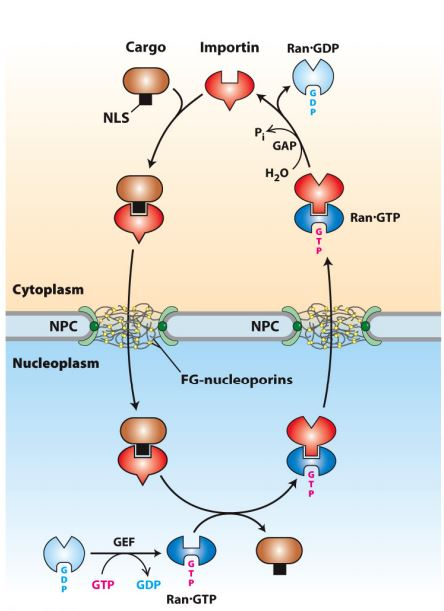
\includegraphics[width=0.5\textwidth]{images/import-exportNucleo.JPG}
                \caption{\small Molecole coinvolte nell'importazione del cargo e nell'esportazione dell'importina con il fine di compiere il ciclo nuovamente}
                \label{fig:mesh1}
            \end{figure}
            
    \subsection{Esportazione}
        \subsubsection{Nuclear Export Sequence}
            NES sta per \textit{nuclear export sequence} ed è una sequenza ricca di leucina (e un percentuali minori isoleucina, valina, metionina e fenialanina).
            
        \subsubsection{Processo esportazione}
            L'esportazione dal nucleo avviene per proteine che veicolano l'uscita di molecole sintetizzate nel nucleo, quali tRNA, mRNA o subunità ribosomiali.\\
            Per l'esportazione dal nucleo sono coinvolte proteine in grado di compiere \textit{shuttling}, ovvero hanno sia una sequenza NLS che NES per essere esportate e importate dopo aver compiuto il loro dovere, tra le quali \textit{exportin1} o \textit{CRM1}.
            \begin{enumerate}
                \item la proteina target espone il NES
                \item la sequenza NES viene associata a exportin1 o CRM1 (nel nucleo)
                \item avviene l'associazione a una RAN-GTP: la formazione del complesso per il trasporto è ora pronto.
                \item attraversamento NPC
                \item GAP promuove idrolisi di GTP di RAN-GTP che rilascia l'esportina, la quale rilascia il cargo.
            \end{enumerate}
            \begin{figure}[h]
                \centering
                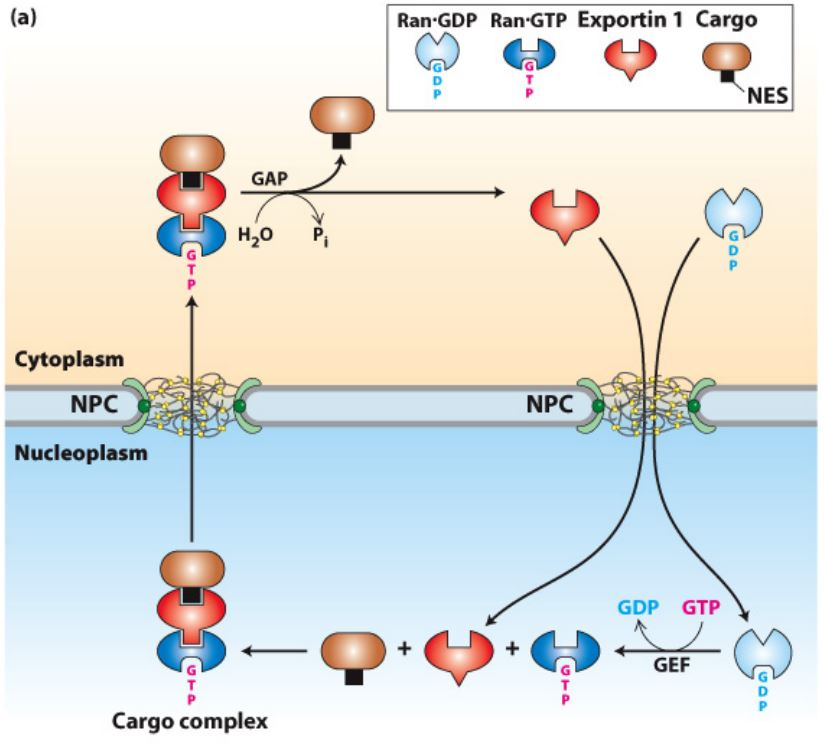
\includegraphics[width=0.5\textwidth]{images/exportNucleo.JPG}
                \caption{\small Molecole coinvolte nell'esportazione}
                \label{fig:mesh1}
            \end{figure}
            
            \textbf{RAN}\\
                RAN, oltre ad avere importanti compiti circa l'import e l'export dal nucleo, assume altri comportamenti in fasi cellulari diverse.\\
                Durante l'interfase protegge la comatina, mentre durante la mitosi fornisce le "coordinate" ai MT per la formazione del fuso mitotico utilizzando GEF e GAP, in prossimità della cromatina infatti c'è una concentrazione maggiore di RAN-GTP.
                
        \subsubsection{Esportazione attiva di mRNA}
            L'mRNA è trascritto nel nucleo e deve essere esportato per essere tradotto.\\
            La sua esportazione è associata a delle RNA binding protein (in particolare NXF1 e NXT1) che hanno propensione ad attraversare la maglia di nucleoporine FG e vengono dissociate dall'mRNA da un RNA-elicasi. 
            L'mRNA, NXF1 e NXT1 sono a questo punto liberi, e l'mRNA si può l'associare ai ribosomi.\\
            Le RNA binging protein possiedono una sequenza NLS che consente loro di essere importate nel nucleo per svolgere nuovamente la loro funzione (shuttling).
            \begin{figure}[h]
                \centering
                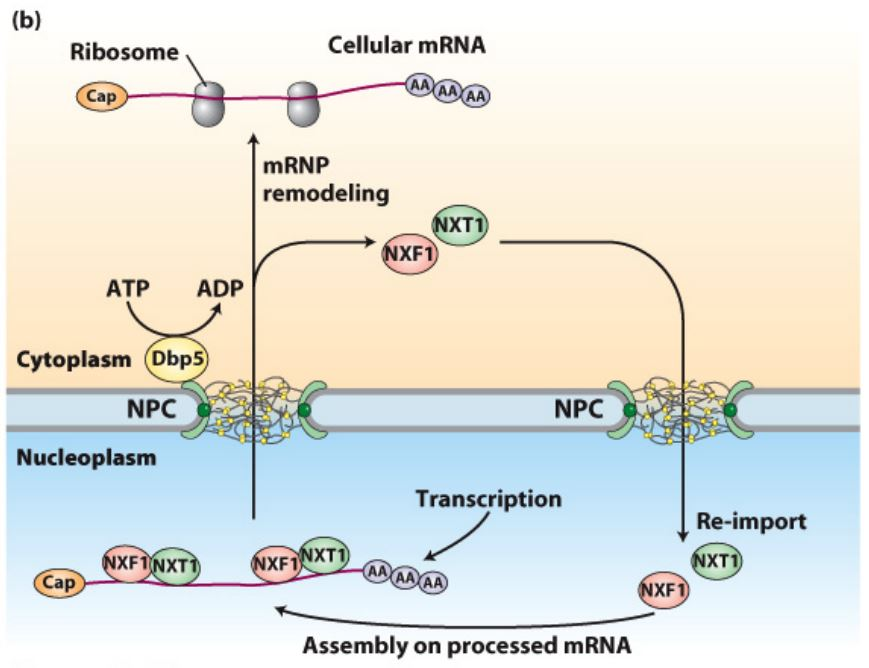
\includegraphics[width=0.5\textwidth]{images/exportNucleomRNA.JPG}
                \caption{\small Molecole coinvolte nell'esportazione si una molecola di mRNA maturo}
                \label{fig:mesh1}
            \end{figure}
    
\section{Destinazione: Mitocondrio}
    Il mitocondrio è un organello cellulare ottenuto dalle cellule eucariotiche per incorporazione di un altro organismo (vedi teoria endosimbiontica). 
    \subsection{Struttura mitocondrio}
        Il mitocondrio è composto da due membrane, la porzione completamente interna è chiamata matrice mitocondriale, lo spazio tra le due viene chiamato spazio intermembrana.\\
        Si occupa della respirazione cellulare e sulla sua membrana sono presenti le proteine che rendono possibile di questo processo. Racchiude il proprio genoma mitocondriale (DNA-M), le proprie RNA-P e tRNA. I complessi proteici codificati dal DNA-M sono composti in maggior parte da porzioni codificate dal DNA-C (cellulare): è pertanto necessario un coordinamento tra i geni del DNA-M e del DNA-C.
        In particolare le proteine sintetizzate nel citoplasma dal DNA-C devono raggiungere il mitocondrio.
        
    \subsection{Mitocondrial Targeting Sequence}
        Per MTS (mitocondrial targeting sequence), si intende una sequenza specifica posta all'N-terminale rappresentata da un $\alpha$E anfipatica di lunghezza variabile. 
        Dopo l'importazione, MTS viene rimossa.
        
    \subsection{Importazione}
        L'importazione nel mitocondrio avviene a livello post-traduzionale con la proteina non conformata tridimensionalmente.\\
        Sono coinvolte le seguenti molecole:
        \begin{itemize}
            \item HSP70: uno chaperon contro il ripiegamento
            \item TOM20 e TOM22: \textit{Traslocone of Outer Mitocondryal membrane} che non coinvolgono GTP
            \item TOM40: un poro generale della membrana esterna
            \item TIM44: \textit{Trascolone of Inner Mitocondryal membrane}
        \end{itemize}
        L'importazione nella matrice mitocondriale avviene secondo i seguenti step:
        \begin{enumerate}
            \item HSP70 riconosce MTS e impedisce alla proteina di ripiegarsi. Per questa operazione viene consumato ATP
            \item TOM20 e TOM22 predispongono la proteina all'importazione esponendo la MTS
            \item TIM44 si allinea a TOM40 spazialmente, per permettere alla proteina di attraversare entrambe le membrane simultaneamente
            \item HSP70 idrolizza ATP per permettere la traslocazione della proteina senza che avvenga un ripiegamento. Perchè avvenga la traslocazione è necessaria la differenza di gradiente protonico tra i lati della membrana.
            \item rimozione della MTS
        \end{enumerate}
        \begin{figure}[h]
            \centering
            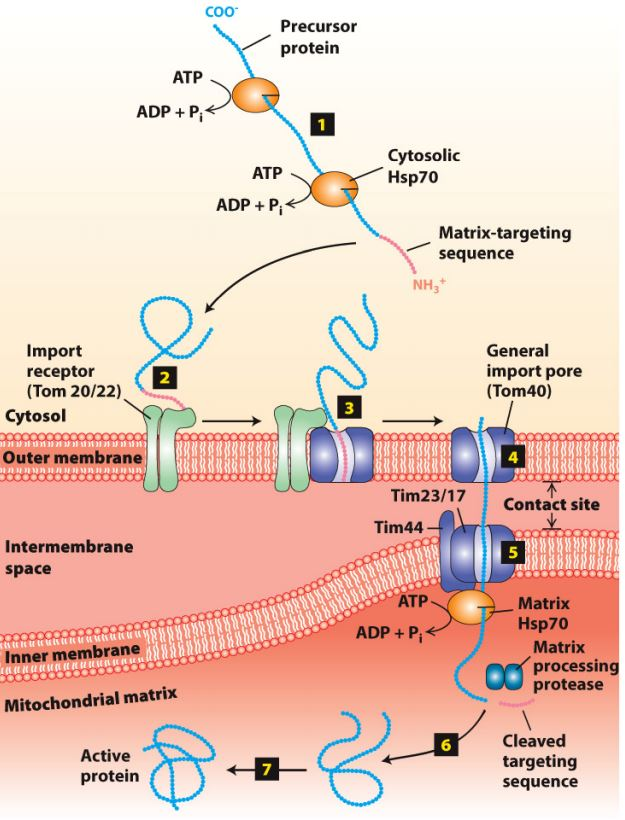
\includegraphics[width=0.7\textwidth]{images/importMito.JPG}
            \caption{\small Molecole coinvolte nell'importazione di una proteina svolta nella matrice mitocondriale}
            \label{fig:mesh1}
        \end{figure}
        
        \subsubsection{Destinazioni nel mitocondrio}
            Essendo un complesso formato da diverse membrane, proteine diverse avranno luoghi interni al mitocondrio differenti. In base alla loro destinazione si evidenzia una sequenza variabile adiacente a MTS.\\
            
            \textbf{Matrice mitocondriale}\\
                Presenta una MTS all'N-terminale, è il procedimento descritto in precedenza.\\
                
            \textbf{Integrali di membrana interna}\\
                Esistono diverse possibilità: 
                \begin{itemize}
                    \item Sequenza MTS all'N-terminale seguita da sequenza topogenica STA che permette l'inserzione nella membrana
                    \item Sequenza MTS all'N-terminale seguite da sequenze riconosciute da OXA1 (a livello della membrana interna, riconosce proteine nella matrice trasferite completamente e le reinseriscono nella membrana).
                    \item Sequenza primaria a-tipica, senza sequenza MTS all'N-terminale, ma con sequenze interne riconosciute da un recettore dedicato TIM. Dopo passaggio attraverso TOM40 c'è un interazione con un complesso TIM dedicato che inserisce la proteina nella membrana.
                \end{itemize}
            
            \textbf{Integrali di membrana esterna}\\
                Riguarda per lo più proteine che assumono la conformazione di barile$\beta$. Avviene grazie alla sequenza MTS all'N-terminale insieme a STA che consentono la diffusione interna al doppio strato lipidico. (TOM40 importa se stesso)\\
            
            \textbf{Spazio intermembrana}\\
                Esitono diverse sequenze che permettono l'arrivo di una proteina nella porzione inetrmembrana:
                \begin{itemize}
                    \item presenza MTS all'N-terminale (passaggio per TOM e successivamente TIM) con sequenza STA. Rilascio della proteina nella membrana interna, intervento di una proteasi che elimina la sequenza transmembrana per liberare la sequenza di AA nello spazio intermembrana.
                    \item presenza di MTS all'N-terminale specifica per il poro generale TOM40. Avviene una semplice diffusione, TIM44 non si allinea. La formazione di ponti disolfuro garantisce l'unidirezionalità del movimento. 
                \end{itemize}
            
\section{Destinazione: Cloroplasto}
    L'incorporazione del cloroplasto nelle cellule vegetali è associata alla stessa teoria endosimbiontica per i mitocondri. Le proteine che lo compongono sono per lo più codificate a livello di DNA-C.
    \subsection{Struttura cloroplasto}
        Il cloroplasto ha un'organizzazione più complessa del mitocondrio: sono sempre presenti le due membrame interna ed esterna, ma al posto della matrice si identifica lo stroma, all'interno del quale ci sono delle organizzazioni a cisterne chiamate tilacoidi.\\
        Solo a livello dei tilacoidi si nota il gradiente protonico citato in precedenza per i mitocondri. 
        
    \subsection{Importazione}
        L'importazione avviene attraverso step e componenti molto simili a quelle del mitocondrio. In particolare TOM diventano TOC (\textit{Traslocone of the Outer Chloroplast membrane}) e TIM diventano TIC (\textit{Traslocone of the Inner Chloroplast membrane}). \\
        La sequenza che determina l'importazione viene detta CTS, \textit{chloroplast transer sequence} che verrà tagliata dopo la traslocazione. CTS e MTS differiscono in larga parte. CTS è ricca di serine, treonine ma povera di acido glutammico e asparagina.\\
        La fonte energetica utilizzata per il trasferimento della proteina è l'ATP per prevenire il ripiegamento (sempre ad opera di HSP70). La proteina per poter transitare non deve essere ripiegata. Non c'è contributo del gradiente protonico per arrivare allo stroma (proprio perchè non c'è gradiente se non a livello dei tilacoidi). \\
        Nel caso una proteina debba raggiungere il tilacoide, esiste un'ulteriore sequenza segnale, riconosciuta da SRP che assieme a SRP receptor promuovono il trasferimento all'interno del tilacoide, successivamente la sequenza viene eliminata.
        Il tilacoide viene raggiunto tramite un canale diverso che permette di traslocare anche proteine non ripiegate. La fonte energetica per questo step è data dal gradiente protonico.

\section{Destinazione: Perossisomi}
    I perossisomi sono delle vescicole che sono adibiti a processare chimicamente delle molecole liberando $H_{2}O_{2}$. Dal momento che questa sostanza risulta tossica e dannosa, si confinano queste reazioni nei perossisomi. 
    I perossisomi sono generalmente sferici e contengono enzimi come l'\textit{ossidasi} e la \textit{catalasi}.\\
    Il metabolismo degli acidi grassi avviene a livello di mitocondrio e di perossisoma dando come risultato le stesse molecole ad eccezione per ATP, NADH e FADH$_{2}$, ma il perossisoma sono produce calore.\\
    L'ingresso della proteina nel perossisoma avviene a livello \textbf{post} traduzionale.
    
    \subsection{Peroxisome Targeting Sequence}
        Ci sono due tipologie di sequenze di targeting per il perossisoma che \textbf{non} venengono rimosse dopo l'importo. 
        La sequenza è \textit{serina-lisina-leucina}. Possiamo differenziare in:
        \begin{itemize}
            \item \textbf{PTS1}: la maggioranza, posta al C-terminale 
            \item \textbf{PTS2}: la minoranza, posta all'N-terminale
        \end{itemize}
        
    \subsection{Importazione}
        L'importazione di una proteina all'interno del perossisoma coinvolge i seguenti elementi:
        \begin{itemize}
            \item PEX5: un recettore sulla membrana citosolica del perossisoma per le PTS
            \item PEX14: proteina integrale di membrana per il trasporto
            \item PEX 10, 2, 12 integrali di membrana per ubiquitinazione
            \item PEX 1, 6, delle AAA ATPasi 
        \end{itemize}
        Questo processo prosegue secondo le fasi (in questo esempio la proteina possiede PTS1):
        \begin{enumerate}
            \item proteina viene interamente tradotta
            \item proteina espone PTS1 e viene riconosciuta dalla tasca dedicata di PEX5
            \item PEX5 interagisce con PEX14 che promuove la traslocazione nel lumen
            \item dissociazione PEX5 dalla proteina. Fino a questo punto non c'è dispendio di energia
            \item Dispendio ATP da parte di PEX 10, 2, 12 che mono-ubiquitinano PEX5
            \item PEX 1, 6 estraggono PEX5 dalla membrana che è libera di compiere di nuovo il suo dovere consumando ATP.
        \end{enumerate}
        Mutazioni distinte delle proteine della famiglia PEX (presenti in pazienti affetti dalla sindrome di Zellveger) hanno permesso di studiare a fondo il fenotipo dei perossisomi.\\
        Ad esempio, mutando PEX12, si assiste alla formazione di perossisomi che però rimangono privi di contenuto. La mutazione di PEX3 invece si manifesta con l'assenza dei perossisomi stessi. 
        \begin{figure}[h]
            \centering
            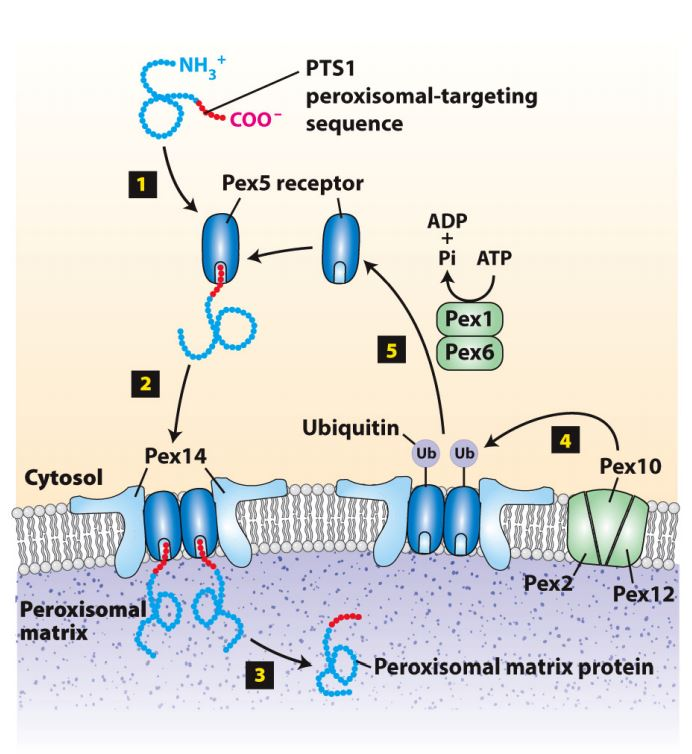
\includegraphics[width=0.5\textwidth]{images/importPerossisoma.JPG}
            \caption{\small Molecole coinvolte nell'importazione di una proteina nel perossisoma}
            \label{fig:mesh1}
        \end{figure}
        
    \subsection{Origine dei perossisomi}
        I perossisomi possono essere generati a partire da perossisomi pre-esistenti (grazie a PEX11) oppure ex-novo per gemmazione di una vescicola del RE. Nel secondo processo concorrono molte proteine della famiglia PEX e PMP70. \\

\section{Maturazione delle proteine}
    Per maturazione delle proteine si intendono eventi che possono avvenire a livello post o co-trazuzionale, vengono trasportate con SEC e avvengono nel RE o nel Golgi.
    
    \subsection{Glicosilazione}
        Per glicosilazione si intende l'aggiunta di componenti saccaridiche alla struttura proteica. Sono modifiche post-traduzionali che avvengono su AA specifici, ovvero serina e treonina (in corrispondenza di un OH nel lumen del Golgi) e asparagina (su un $NH_{2}$ nel lumen de RE).  \\
        La glicosilazione nel RE (\textit{N-linked glycosylation}) avviene seguendo gli step:
        \begin{enumerate}
            \item formazione del precursore con zuccheri (14 monomeri) assemblati covalentemente per la formazione del \textit{dolicolofosfato}, il precursore della glicosilazione vera e propria (associato ad asparagina)
            \item in presenza della sequenza segnale asparagina-x-serina/treonina avviene una glicosilazione a livello cotraduzionale degli N-terminali
        \end{enumerate}
        Alcuni step sono reversibili.\\
        La glicosilazione è necessaria al ripiegamento. La modifica degli zuccheri indicano infatti il corretto ripiegamento o servono alla recluta di chaperon per arrivare ad una conformazione corretta. Questa modifica è anche utile per la segnalazione della degradazione del polipeptide tramite l'albero saccaridico. 
        \begin{figure}[h]
            \centering
            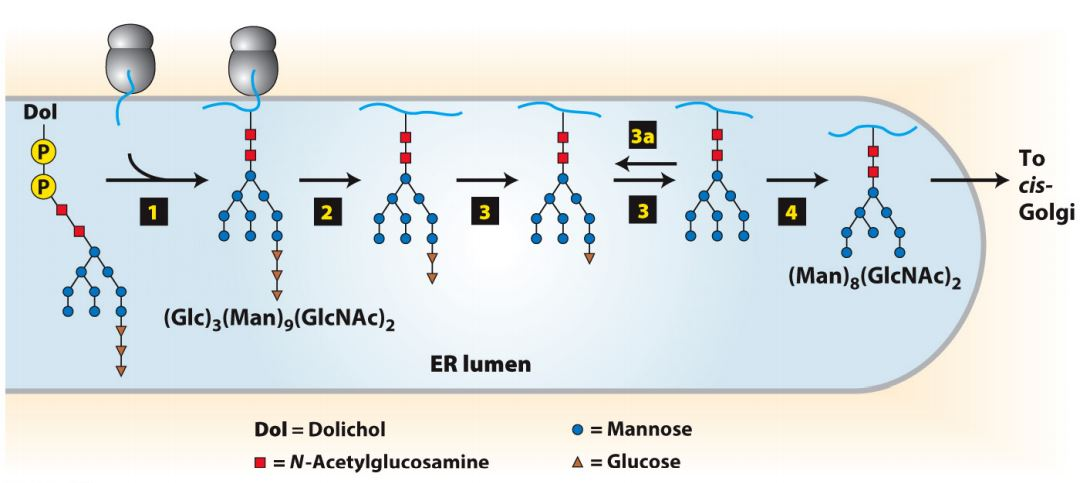
\includegraphics[width=0.7\textwidth]{images/glicosilazine.JPG}
            \caption{\small Glicosilazione di una proteina}
            \label{fig:mesh1}
        \end{figure}
        
    \subsection{Ponti disolfuro}
        I ponti disolfuro sono legami tra catene tra residui AA di cisteine che vengono effettuate solo a livello del lumen del RE.
        Viene mediato dall'enzima disolfuro-isomerasi (PDI) che contiene cisteine e un ponte disolfuro. \\
        La reazione è composta da due REDOX :
        \begin{enumerate}
            \item avviene una reazione tra PDI e una cisteina della proteina target che produce il ponte disolfuro
            \item avviene una reazione tra due cisteine del peptide target rilasciando PDI (grazie a potere dell'ossidazione) e spostando il ponte disolfuro tra i due residui AA
        \end{enumerate}
        La PDI può promuovere anche la rilocazione del ponte disolfuro.\\

        \begin{figure}[h]
            \centering
            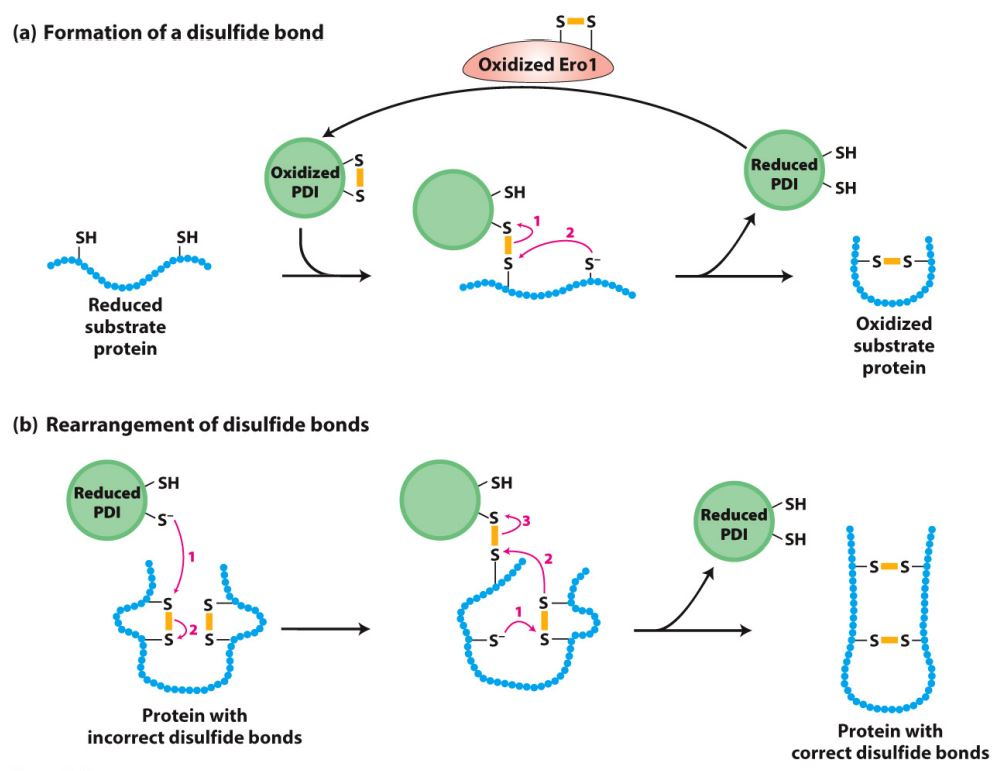
\includegraphics[width=0.6\textwidth]{images/pontiDisolfuro.JPG}
            \caption{\small Formazione dei ponti disolfuro e rilocazione attraverso PDI}
            \label{fig:mesh1}
        \end{figure}
        
    \subsection{Folding e assemblaggio di complessi multiproteici}
        Il folding e l'assemblaggio sono eventi che si verificano nel lumen del RE. 
        \subsubsection{Emoagglutinina del virus influenzale (HA)}
            Prendiamo come esempio il processo di assemblaggio della proteina che funge da antigene sul capside del virus influenzale. 
            \begin{enumerate}
                \item la proteina HA possiede una seguenza target all'N-terminale che permette l'accesso al RE. 
                \item avviene una glicosilazione cotraduzionale per ogni sequenza utile transitata: quest'operazione è utile al processo di folding che verrà effettuato dallo chaperon BiP.
                \item PDI forma dei ponti disolfuro
                \item la proteina di associa con altre proteine (calnexina e calreticolina) che legano specifici gruppi funzionali degli zuccheri, in questo modo la proteina viene ritenuta dal RE e non passerà attraverso il Golgi
                \item in corrispondenza della sequenza STA (Stop Tranfer Anchor) la proteina viene rilasciata nella membrana lipidica 
                \item la proteina funzionale è composta da un trimero, per questo motivo avverrà un riassemblaggio strutturale 
                \item proteolisi per la formazione di HA matura e fuoriuscita dal RE
            \end{enumerate}
                \begin{figure}[h]
                \centering
                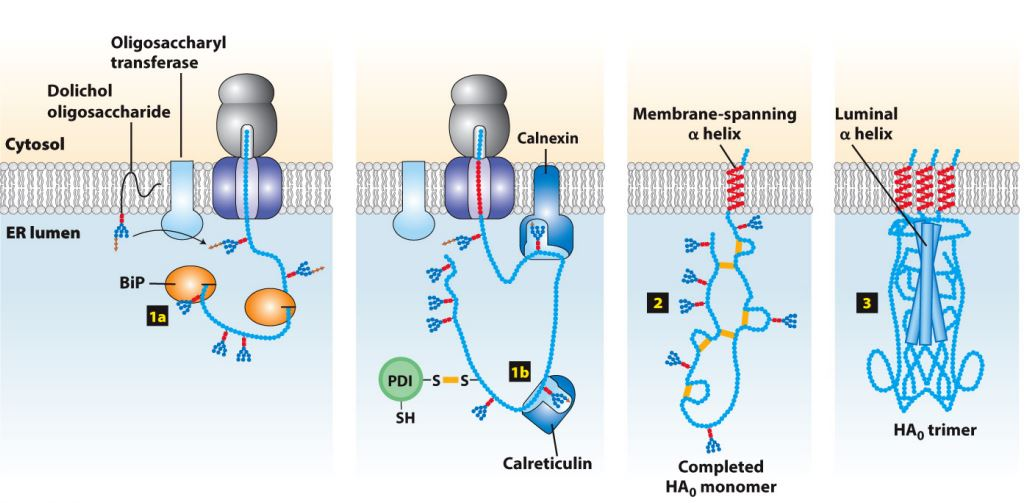
\includegraphics[width=0.7\textwidth]{images/ripiegamentoHA.JPG}
                \caption{\small Ripiegamento dell'emoagglutinina}
                \label{fig:mesh1}
            \end{figure}
        
        
        \subsubsection{Isomerizzazione della prolina}
            I carboni attorno ai legami peptidici assumono solamente dei determinati angoli, alcuni dei quali sono incompatibili con la formazione di strutture tridimensionali corrette (incompatibili con la formazione di determinate strutture secondarie). 
            Per questo motivo intervengono delle cis-trans-isomerasi (abbondanti nel lumen del RE) che catalizzano lo scambio conformazionale tra isomeri cis e trans.
        
        \subsubsection{Proteine mal-ripiegate}
            Le proteine non ripiegate correttamente non vengono rilevate come mature, per questo motivo non possono lasciare il RE e si crea un accumulo di materiale. L'accumulo causa a sua volta stress signaling.\\
            Esistono diversi metodi per controllare il corretto ripiegamento delle proteine, tramite quello che si chiama \textit{unfolded protein response} (UPR) tra cui il comportamento di Ire1.
            \begin{enumerate}
                \item Lo chaperon BiP cerca di ripiegare correttamente le proteine. Quando non è impegnato in questo compito, BiP è associato alla proteina di membrana Ire1.
                Quando la concentrazione di BiP libera è altra, Ire1 non vi è associata e genera un segnale citoplasmatico tramite un mRNA per cui lo "splicing" non è completato (Hac1).
                \item Ire1 ad effettua le modifiche a questo mRNA per farlo maturare (attua un'attività nucleosidica su un introne anomalo)
                \item traduzione del mRNA per ottenere altri chaperon BiP.
            \end{enumerate}
            Ire1 assume anche altri compiti, per esempio la sua alterata espressione genica collabora al signaling per la morte cellulare, infatti fa maturare miRNA per la regolazione della traduzione del gene pro-apoptotico.\\
            La situazione di stress signaling prodotta dall'accumulo di proteine malripiegate è spesso utilizzata sperimentalmente utilizzando la tunicamicina (un antibiotico che blocca le modifiche all'ancora lipidica necessaria al processo di glicosilazione).\\
            
    \subsection{Degradazione proreica}
    \begin{figure}[h]
            \centering
            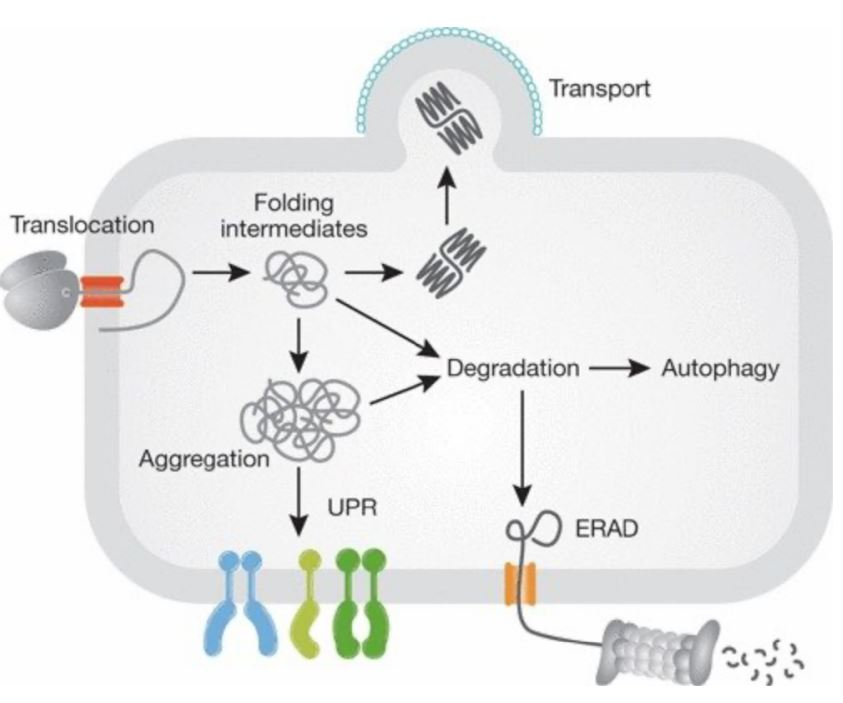
\includegraphics[width=0.5\textwidth]{images/degradazione.JPG}
            \caption{\small Diversi destini per proteine ripiegate e mal-ripiegate}
            \label{fig:mesh1}
        \end{figure}
        La degradazione delle proteine può avvenire tramite metodi che differiscono dall'utilizzo del proteasoma. Per l'operazione che si descrive ora si necessita della traslocazione dal lumen al citosol.\\
        L'enzima mannosidasi marca le proteine che necessitano di traslocazione nel citosol (dislocazione non per proteine glicosilate). Oltre alla mannosidasi esitono altri metodi per la traslocazione (di proteine glicosilate) che però non sono noti.\\
        Esiste un complesso chiamato ERAD (ER associated degradation), formato da 4 proteine integrali di membrana che insieme a p97 (AAA-ATPasi) strappa proteine destinata alla degradazione dalla membrana del RE. \\
        Se questo processo non va per il meglio si può attivare un UPR, altrimenti interviene ERAD fa passare le proteine nel citosol e contemporaneamente le poliubiquitina.
        

\pagebreak
\setcounter{section}{0}

\large{\addcontentsline{toc}{part}{Capitolo 8: Traffico vescicolare}}
\Huge\textbf{Capitolo 8: \\Traffico vescicolare}\\

\small
\section{Reticolo endoplasmatico, Golgi e Lisosoma}
    Il RE è in diretta continuità con la membrana nucleare e comunica fortemente con il Golgi. Il trasporto tra RE e Golgi è mediato da vescicole. Dal RE si spostano le proteine mature pronte ad essere modificate o esportate dal Golgi.\\
    Se la proteina non possiede sequenze particolari (viste nel capitolo precendente) vengono veicolare dal RE al Golgi.
    Per trasporto anterogrado di una proteina di intende il trasporto da RE, passando per Golgi per essere poi espulsa dalla membrana.\\
    Per trasporto retrogrado si intende il percorso contrario e avviene per una determinata classe di proteine.
    
    \subsection{Golgi}
        Il Golgi è costituito da cinque cisterne (più grande delle vescicole stesse) che prendono nomi diversi in base alla propria posizione. A partire dal quella prossima al RE sono:
        \begin{itemize}
            \item Cis Golgi Network (CGN)
            \item Cis Golgi (CG)
            \item Media Golgi (MG)
            \item Trans Golgi (TG)
            \item Trans Golgi Network (TGN)
        \end{itemize}
        Essendo prossima alla membrana plasmatica, TGN è la cisterna che funge da "smistatore" per le vescicole in uscita dalla cellula (o comunque le sostanze arrivate fino a lì) generando vescicole diverse per destinazione diverse. 
        Determina l'identità del compartimento di destinazione.\\
        Il contenuto di una vescicola da cisterna a cisterna muta gradualmente, non abbiamo la generazione di nuove vescicole mano a mano. Muta invece la composizione chimica interna.
        \begin{figure}[h]
            \centering
            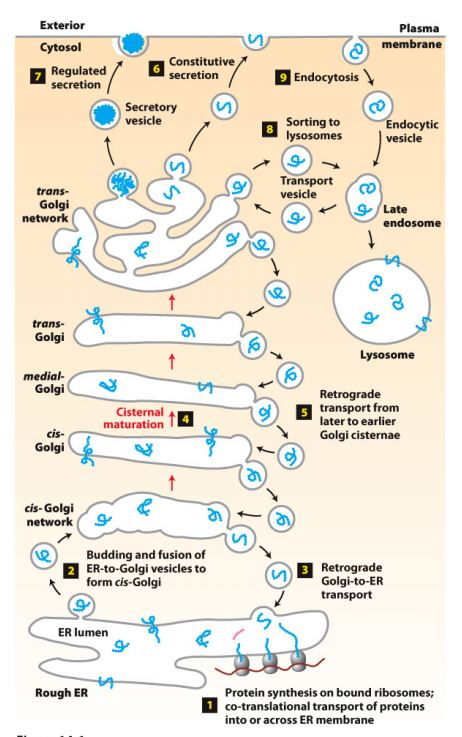
\includegraphics[width=0.5\textwidth]{images/Golgi.JPG}
            \caption{\small Schema della struttura del Golgi, si noti come TGN è deputata alla realizzazione di diverse tipologie di vescicole}
            \label{fig:mesh1}
        \end{figure}
            \subsubsection{Funzioni}
            Il Golgi è adibito alla glicosilazione delle proteine. Questo processo inizia nel CGN e la modifica prende parte in cisterne diverse con step graduali fino ad arrivare al TGN. \\
            Il Golgi contiene delle proteine residenti quali glicosidasi e glicosiltransferasi per adempiere alla propria funzione di glicosilare i peptidi.
            
    \subsection{Lisosoma}
        Il lisosoma è un componente cellulare vescicolare che si occupa della degradazione di materiali per lo più extracellulari, batteri o organelli non più in grado si svolgere il proprio compito. Ha quindi una funzione catabolica. La fusione dell'endosoma tardivo con un lisosoma determina la degradazione del suo contenuto.\\
        Il lisosoma possiede un pH acido per consentire alle idrolasi acide di svolgere il proprio compito, per questo motivo presenta delle pompe protoniche per mantenere questo livello di acidità. 
            
    \subsection{Esperimenti}
        \subsubsection{VSV-G}
            L'obiettivo è visualizzare la proteina virale VSV-G (proteina di superficie) che da neosintetizzata di trova nel RE. Dopo 40 minuti si ritrova nel Golgi mentre dopo 30 ore si trova nella membrana.\\ 
            Per fare ciò viene utilizzata una GFP, una proteina naturale che riesce a effettuare un processo di bioluminescenza.\\
            La cellula produce VSV-G in un singolo istante perchè la proteina (modificata, non wt) è sensibile alla temperatura. Quindi questa variante è più prona a non ripiegarsi correttamente a una temperatura più elevata del normale (\textit{temperatura non permissiva}). 
            Qualora la proteina non fosse ripiegata correttamente non viene trasportata.\\
            Le cellule vengono spostate alla temperatura permissiva, la proteina ri ripiega correttamente e viene rilasciata dal RE verso il Golgi e via dicendo.
            
        \subsubsection{Mutanti deficitari}
            I mutanti deficitari sono mutanti con impedimenti di specifiche funzioni coinvolte nei processi interposti tra la sintesi e l'espulsione dalla membrana. \\
            Sono stati ampiamente utilizzati tramite cellule di lievito. Queste funzioni sono essenziali per la vita, di conseguenza sono stati selezionati mutanti temperatura sensibili.\\
            La classe di mutanti A, posti alla temperatura non permissiva accumulano proteine secretorie nel citosol, quindi la funzione difettiva consisteva nell'importo nell'ER (mutanti SEC).\\
            Altre classi di mutanti accumulano proteine nel lumen dell'ER (deficit nella gemmazione), accumulano proteine nelle vescicole di connessione ER - Golgi, accumulo nel Golgi.\\
            Incrociando mutanti diversi si possono osservare fenotipi che sono stati essenziali allo studio di questi eventi.

\section{Gemmazione e fusione}
    \subsection{Coat Proteins}
        La gemmazione delle vescicole è guidata dalle Coat Proteins (CP). Sono queste proteine a dettare una curvatura della membrana associandosi ad essa.\\
        Le CP hanno interazioni specifiche con proteine trans membrana e GTPasi associate. La deformazione della membrana determina la formazione di una protrusione che alla fine si distaccherà.
        Una volta che la vescicola è stata formata si procede a un disassemblaggio delle CP prima che essa arrivi alla propria destinazione.\\
        Esistono vari tipi di CP, i quali determinano la tipologia delle vescicole:
        \begin{itemize}
            \item COP1 (con ARF): impiegata nel trasporto retrogrado. ARF è una GTP binding-protein.
            \item COP2 (con SAR1): impiegata nel trasporto anterogrado. SAR1 è una GTPasi che induce gemmazione qualora sia associata al foglietto citosolico e recluta membri di COP2 per la vescicolazione, nel momento in cui il GTP viene idrolizzato si induce il distacco dei COP1.
            \item Clatrina (con ARF)
        \end{itemize}
        SAR1 e ARF sono presenti a livello citoplasmatico associate a GDP quindi inattive.\\
        Non è nota la CP specifica per il trasporto da TGN alla membrana cellulare.\\
        Vari esperimenti hanno confermato la necessaria presenza delle CP per la formazione delle vescicole e della necessità di avere un'idrolisi di GTP per il rilascio del coat (per il secondo esperimento si utilizza GTP$\gamma$s il quale non permette idrolisi).
        
    \subsection{Gemmazione con COP2}
        A livello citoplasmatico SAR1 è libera finchè SEC12 non interagisce come GEF: SAR1 viene "caricata" con GTP facendo esporre il proprio N-terminale idrofobo. Questo fa sì che SAR1 si associ al foglietto citosolico della membrana. \\
        Questa associazione determina la recluta di altri componenti proteici di COP2 che vanno a formare la vescicola. Nel momento in cui il GTP di SAR1 viene idrolizzato (GAP), il coat si disassembla e la vescicola rimane nuda.
        
    \subsection{Clatrina}
        La clatrina è un dipeptide, tre di questi dipeptidi formano una struttura a triscele. 36 trisceli formano una struttura sferica attorno a una vescicola. 
        La clatrina non sa interagire autonomamente con la vescicola, ma ha bisogno di un'adattina, una proteina che consente l'interazione con la membrana.\\
        Il distacco della vescicola che si forma in presenza della clatrina è operata dalla dinamina. La dinamina è una proteina che opera una "strozzatura" del collo della gemma corrispondente alla nuova vescicola e ne determina il distacco effettivo. La dinamina è di per sè una GTPasi multimerica, di conseguenza questo processo energicamente sfavorito è realizzabile spendendo GTP. 
        Non si conoscono proteine analoghe per gli atri tipi di CP.
    
    \subsection{Adattina}
        Le adattine (adapter proteins) sono una classe di proteine che aiutano la clatrina a formare la struttura sferica per la vescicola (per esempio AP1, GGA e AP2).\\
        Un particolare adattina riesce anche interagire direttamente con la vescicola e formare un coat autonomo in assenza della clatrina (AP3 complex).
        
        
    \subsection{Fusione}
        La fusione della vescicola con CGN avviene grazie all'interazione di proteine specifiche chiamate\textbf{ V-SNARE}, presenti sulla vescicola, e \textbf{T-SNARE}, presenti sulla membrana target.\\
        Entrambe le SNARE sono proteine costituite da coiled coil specificamente molto affini tra loro. La loro interazione promuove la giustapposizione dei foglietti citosolici. 
        L'avvicinamento e la fusione delle membrane non è un processo energicamente favorito, tuttavia l'interazione delle proteine citate sopra, consente di superare la barriera energetica e di compiere la fusione.\\
        L'esposizione delle V-SNARE avviene dopo la perdita delle CP. Esistono circa 20 diverse tipologie di V e T-SNARE specifiche per l'interazione di determinate membrane di origine con determinate membrane target.\\
        La dissociazione dei coiled coil che si formano per la fusione richiede energia, per questono intervengono delle AAA-ATPasi.\\
        
        In particolare, le V-SNARE presenti su TGN sono chiamate VAMP mentre le T-SNARE della membrana sono sintaxina e SNAP25. La fusione alla membrana plasmatica avviene attraverso l'interazione di 4 polipeptidi (VAMP, sintaxina e due molecole di SNAP25).\\
        
        A livello vescicolare è presente anche una GTPasi della famiglia delle \textit{RAB}. Ogni RAB caratterizza una membrana di origine e determina specificità con la destinazione. 
        Le RAB hanno un ciclo specifico di associazione a GTP e GDP, qualora la vescicola sia "in cerca" della membrana target è associata al GTP. GEF e GAP si occupano del cambio dell'attività delle RAB.
        \begin{figure}[h]
            \centering
            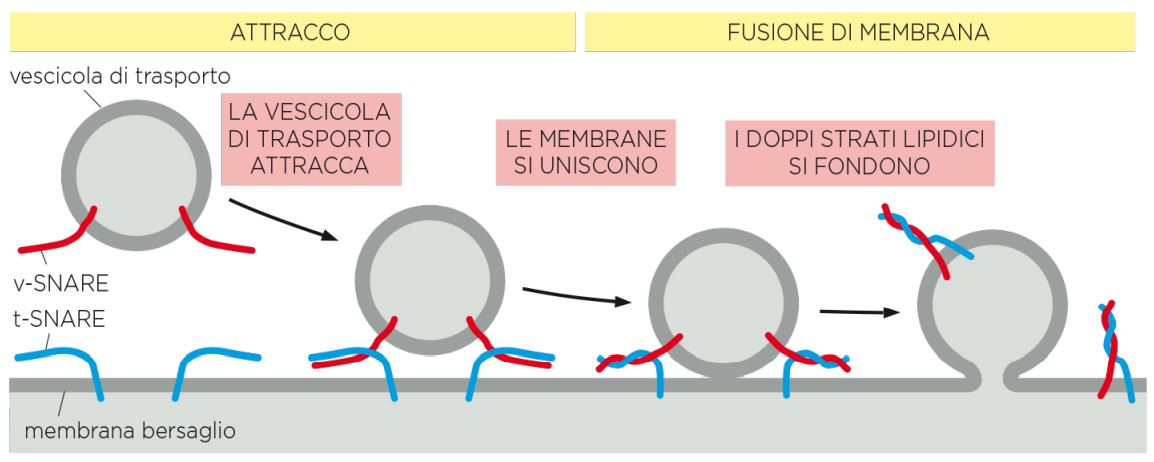
\includegraphics[width=0.8\textwidth]{images/VTSNARE.JPG}
            \caption{\small Interazione T-SNARE e V-SNARE}
            \label{fig:mesh1}
        \end{figure}
    
\section{Trasporto RE - CGN}
    Le proteine presenti sulla membrana interagiscono con componenti esterni per la formazione del coat, tuttavia esistono anche elementi proteici che si interfacciano con l'interno della vescicola con i cargo solubili. \\
    Come è facile immaginare, è proprio in dipendenza del cargo che una vescicola avrà un certo target.
    \subsection{Proteine e COP2}
        Come visto in precedenza, la formazione di del coat tramite COP2 avviene con il fine di avviare un trasporto anterogrado. \\
        La formazione del coat avviene grazie alla presenza di due SEC (23 e 24) che fungono da etichetta specifica per il target da RE a Golgi. SEC24 lega una coda proteica della proteina di membrana del RE (serve comunque l'interazione con SAR1-GTP).\\
        La coda di AA segnale esposta sul lato citoplasmatico che viene legata determina l'interazione con le proteine per il coating.\\
        Dopo questo passaggio saranno reclutati gli altri membri proteici per la formazione del coat.
        
    \subsection{Proteine e cargo solubili}
        Le proteine solubili cargo hanno sequenze AA specifiche per l'interazione con il recettore di riferimento.
        \subsubsection{Sequenza KDEL e trasporto retrogrado}
            La sequenza KDEL (lisina, asparagina, acido glutammico e leucina) è una sequenza segnale posta al C-terminale del cargo solubile tipica delle proteine luminali del RE.\\ 
            Questa sequenza codifica il fatto che la proteina deve rimanere nel lumen del RE.\\
            La sequenza KDEL possiede un recettore presente sulla membrana del Golgi: infatti nel caso in cui la proteina venga inclusa per caso in una vescicola e arrivi al Golgi, questa verrà identificata dal suo recettore che indurrà la formazione di una nuova vescicola che compierà del lavoro retrogrado per riportare la proteina con KDEL nel RE. 
            La vescicola che torna verso il RE sarà ricoperta da COP1. \\
            Una volta che la vescicola che viaggia dal Golgi verso il RE si è fusa con la membrana del RE, il recettore per KDEL si troverà associato alla membrana del RE. Tuttavia, la proteina con KDEL non interagirà con il suo recettore perchè l'associazione dipende dal gradiente protonico. Il Golgi ha una concentrazione di H$^{+}$ più elevata rispetto al RE, il quale pH induce in cambio di carica da parte della sequenza KDEL che si associa al suo recettore.
            Nel RE, il pH è più alto e questa associazione non avviene.\\
            Lo chaperon BiP è un esempio di proteina con sequenza KDEL.
            \begin{figure}[h]
                \centering
                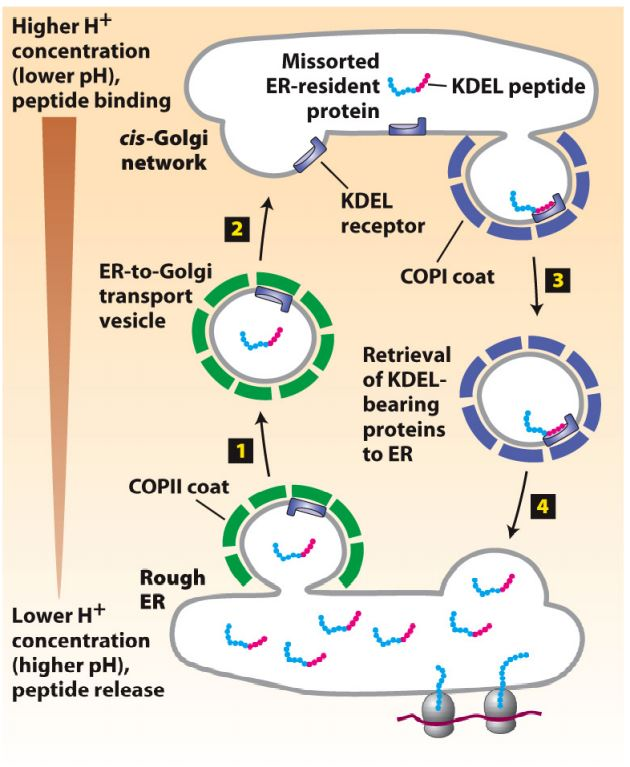
\includegraphics[width=0.5\textwidth]{images/KDEL.JPG}
                \caption{\small Trasporto erroneo anterogrado di proteina con KDEL e conseguente trasporto retrogrado}
                \label{fig:mesh1}
            \end{figure}

\section{Trasporto tra le cisterne del Golgi}
    Le cisterne del Golgi hanno contenuto e funzioni diverse in base alla loro locazione. Nel momento in cui una vescicola transita attraverso le cisterne cambia gradualmente chimicamente, seguendo un climax dettato dalle cisterne stesse.\\
    In senso anterogrado, la cisterna matura interamente senza gemmazione e fusione.\\
    In senso retrogrado c'è vescicolazione.

\section{Smistamento destinazioni del TGN}
    Il TGN, come detto in precedenza, svolge la funzione di indirizzare vescicole diverse a in direzioni specifiche. In particolare ci sono cinque path possibili che una vescicola può intraprendere:
    \begin{enumerate}
        \item esositosi costitutiva (tramite membrana)
        \item esocitosi specifica (tramite membrana)
        \item lisosoma, con APcomplex
        \item trasporto retrogrado, con COP1
        \item endosoma tardivo (ET) con Clatrina e APcomplex
    \end{enumerate}
    In alcune cellule con tipologie di membrana plasmatica ben differenziate (come le cellule epiteliali), il TGN riesce a direzionare vescicole diverse con cargo diverse per membrane diverse. 
    Lo studio di questo fenomeno è stato condotto utilizzando due virus diversi (HA dell'influenza e VSV-G) che vengono direzionate a due membrane opposte: questo suggerisce che le proteine hanno racchiuso in se stesse i segnali per essere veicolate alla membrana corretta.
    
    \subsection{Targeting del lisosoma}
        Anche le proteine solubili che devono risiedere nel lisosoma possiedono un segnale specifico: possiedono in particolare un gruppo mannosio 6-fosfato legato a una catena di glicosilazione posta in prossimità all'N-terminale (glicosilazione avviene nel CG).
        Presentano questo tipo di struttura le proteine che devono rimanere confinate nel lisosoma per garantirne la funzionalità come gli enzimi lisosomali.\\
        Di seguito il procedimento per trasportare queste proteine al lisosoma:
        \begin{enumerate}
            \item Il segnale viene letto da un recettore specifico per mannosio 6P del TGN
            \item Si forma la vescicola (clatrina)
            \item La vescicola perde le CP (clatrina)
            \item Fusione con ET
            \item ET promuove eventi di fusione per l'accesso al lisosoma
        \end{enumerate}
        Esistono delle molecole con dei marker di mannosio-6P a livello esocellulare per recuperare sostanze che sono finite erroneamente fuori dalla cellula (utilizzando lo stesso recettore), questo stesso pathway promuove la formazione di vescicole coperte da clatrina con dinamina. 

\section{Endocitosi di LDL}
    L'endocitosi è un processo che viene effettuato tramite vescicole di clatrina, AP2 e dinamina.\\
    La regolazione dell'associazione al recettore AP2 può avvenire anche in assenza del ligando nonostante l'associazione sia più stabile e duratura qualora esso sia presente. Queste vescicole possono veicolare diversi carghi, quindi sono presenti molti recettori.  \\
    Per LDL (low density lipoprotein) è destinato a essere degradato dal lisosoma per rendere disponibili i singoli componenti molecolari alla cellula. 
    LDL possiede un recettore specifico ApoB (Apolipoprpteina B) che presenta un cuore altamente idrofobico per legare le componenti lipidiche di LDL (colesterolo e trigliceridi) e un segnale per il recettore. \\
    Sarà il pH a determinare l'associazione tra ApoB e il suo recettore, in particolare:
    \begin{itemize}
        \item nel caso di pH neutro il braccio legante si associa a ApoB
        \item nel caso di pH acido (ET) il braccio si ripiega su se stesso impedendo il legame con ApoB
    \end{itemize}
    L'endocitosi di LDL è determinata da una sequenza target di AA comune per i componenti molecolari che sono destinati all'endocitosi. \\
    Persone con ipercolesterolemia (non dovute direttamente a una dieta malsana) hanno un recettore per ApoB che non riconosce la sequenza corretta, impedendo la corretta encoditosi di LDL.

\section{Degradazione lisosomiale}
    Le proteine che devono essere degradate tramite un lisosoma possono accedervi secondo due vie: la prima interessa le proteine trans-membrana che possono essere degradate o diventare componente della membrana del lisosoma, la seconda interessa componenti solubili citosolici  (ovvero il processo di autofagia).
    
    \subsection{Proteine trans-membrana}
        \subsubsection{Proteine destinate alla degradazione}
            Queste proteine sono quelle che sono state precedentemente mono-UB, processo catalizzato da complessi proteici chiamati ESCRT assieme a ATPasi e VPS4.
            Le proteine destinate alla mera degradazione interagiscono con clatrina e AP2. Nell'ET avviene la formazione di molteplici vescicole (il cui interno è porzione di citoplasma) che contengono tali proteine. 
            Nel momento in cui avviene la fusione con il lisosoma, le vescicole si ritroveranno nell'ambiente acido, la membrana verrà disciolta e con essa anche la proteina.
        \subsubsection{Proteine destinate alla membrana del lisosoma}
            Le proteine destinate alla membrana del lisosoma non vengono incluse nelle vescicole che si formano all'interno dell'ET, ma rimangono invece sulla membrana estrerna. Al momento della fusione, la membrana dell'ET si fonde con quella del lisosoma e le proteine in questione faranno ora parte della membrana del lisosoma.
        \begin{figure}[h]
            \centering
            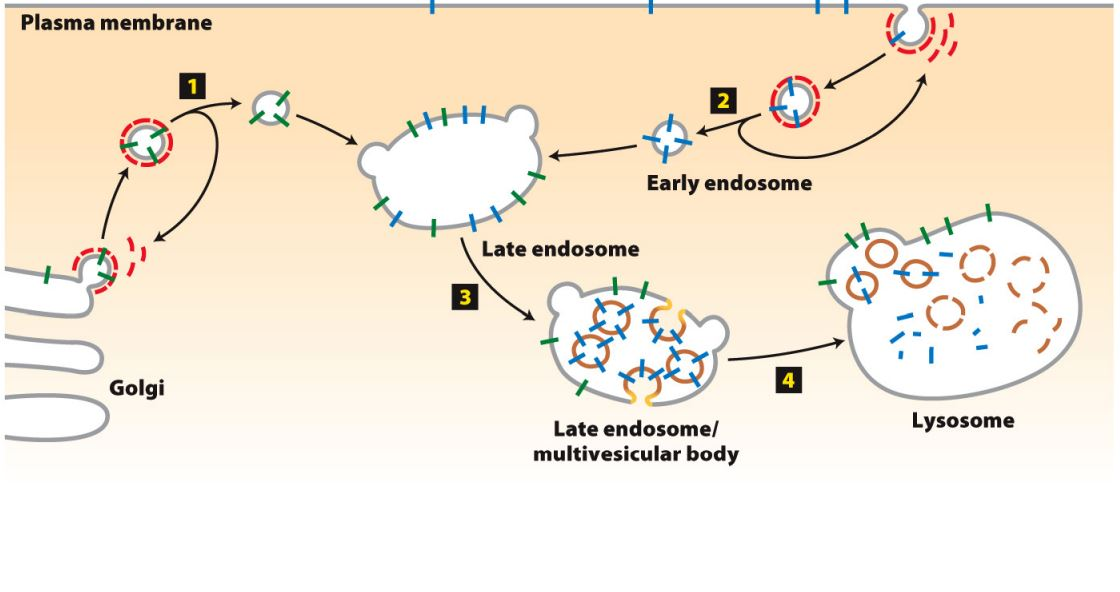
\includegraphics[width=1\textwidth]{images/degradazioneLisosoma.JPG}
            \caption{\small Proteine destinate alla degradazione in blu, proteine destinate alla membrana del lisosoma in verde}
            \label{fig:mesh1}
        \end{figure}
    \subsection{Componenti cistosolici solubili}
        Il processo di degradazione di componenti citosoloci solubili è detto anche autofagia. Questo processo è coinvolto in diverse situazioni: 
        \begin{enumerate}
            \item degradazione di componenti cellulari vecchi o non funzionanti
            \item degradazione di altri contenuti proteici presenti nel citosol
            \item degradazione di porzioni citosoliche in caso di carenze metaboliche
        \end{enumerate}
        I polipeptidi coinvolti nel processo di autofagia (1 e 3) sono i medesimi. In particolare analizzando il caso del lievito, si nota che sono presenti una famiglia di proteine chiamata ATG (autophagy) di cui in particolare fa parte ATG8. 
        ATG8 (nelle cellule umane l'analoga è chiamata LC3) è un peptide presente in due forme: solubile e associato alla membrana (quindi con componente lipidica). 
        ATG8 coopera con le membrane pre-esistenti per la formazione di una "capsula" a doppio strato fosfolipidico attorno alla porzione di citosol/organello da degradare chiamata \textit{autofagosoma}.\\
        L'autofagosoma viene quindi incluso nel lisosoma e ne viene degradato il contenuto.
        \begin{figure}[h]
            \centering
            \includegraphics[width=1\textwidth]{images/Autofagia.JPG}
            \caption{\small Processo di autofagia per un organello e per porzioni di citoplasma}
            \label{fig:mesh1}
        \end{figure}
        
\pagebreak

\setcounter{section}{0}

\large{\addcontentsline{toc}{part}{Capitolo 9: Divisione cellulare}}
\Huge\textbf{Capitolo 9: \\Divisione cellulare}\\

\small
\section{Overview}
    Il ciclo cellulare è il processo per cui una cellula va incontro a una divisione tale per cui si ottengono in ultimo due cellule analoghe. Si divide in due fasi, l'interfase (I), e la mitosi (M). La fase I si divide in G0, G1, S e G2 (in G1, G2 e G3, G sta per \textit{gap}).\\
    Durante la fase S abbiamo la duplicazione del DNA e del centrosoma.\\
    Durante la fase M abbiamo l'effettiva separazione in due cellule figlie.\\
    Durante le fasi G1 e G2 abbiamo accrescimento del volume cellulare e dei suoi componenti. In G2 viene inoltre effettuata divisione mitocondriale.
    Divisione e duplicazione di organelli diversi da centrosoma e eventi diversi dalla duplicazione del materiale genetico sono meno critici per la cellula.
    
    \vspace{0.5cm}
    Il corpo umano è composto di circa $10^{14}$ cellule e ogni giorno se ne rigenerano circa $10^{12}$. Nel corso di una vita si assiste a circa $10^{16}$ divisioni cellulari. 
    Da questi numeri è facile intuire quanto questo processo debba essere controllato e preciso al fine di preservare la vita dell'organismo.\\
    Le componenti che determinano il corretto funzionamento del ciclo cellulare sono un \textit{clock} e un sistema di correzione degli errori (\textit{checkpoints}).
    
    \subsection{Divisione per cellule differenti}
        In tipologie di cellule differenti, velocità e caratteristiche del processo possono essere specifiche. In particolare:
        \begin{itemize}
            \item \textbf{divisione delle cellule embrionali in fasi precoci}:
                \begin{itemize}
                    \item sono divisioni che avvengono molto velocemente, da 30 a 60 minuti per divisione, questo perchè vengono saltate le fasi G1 e G2
                    \item non c'è accrescimento volumetrico delle cellule, sommando il volume occupato dalle figlie si ottiene lo stesso volume della cellula madre
                    \item non c'è controllo a livello di sintesi proteica, errori in questa fase causano la morte embrionale
                    \item il clock della situazione sono i processi di produzione, modificazione e degradazione delle proteine
                    \item non c'è trascrizione di mRNA
                \end{itemize}
            \item \textbf{somatiche}:
                \begin{itemize}
                    \item hanno un ciclo di circa 24 ore
                    \item questa duplicazione è sincronizzata all'accrescimento in volume
                    \item il controllo della produzione, modifica e degradazione delle proteine determina il clock biologico, assieme alla regolazione della trascrizione dell'mRNA.
                    \item è un processo molto controllato, la cellula può generare segnali per indicare il proprio suicidio
                \end{itemize}
            \item \textbf{embrione avanzato}:
                \begin{itemize}
                    \item le cellule interagiscono con l'ambiente
                    \item si differenziano in tessuti e organi diversi
                \end{itemize}
        \end{itemize}
        Le fasi G1 e G2 sono "accessorie": infatti nella fase embrionale precoce viene completamente saltata. G1 e G2 sono responsabili per l'accrescimento della cellula e per il "controllo qualità". \\
        Per controllo qualità si intendono degli eventi che avvengono per fare in modo che la duplicazione vada a buon fine, ovvero START, il controllo della duplicazione del DNA e l'allineamento dei cromosomi sulla piastra metafasica.
        \subsubsection{START}
            Uno dei controlli che viene effettuato dalla cellula a monte della sua divisione è controllare che siano disponibili una quantità sufficiente di sostanze nutritive. 
            Se questo controllo va a buon fine, allora si inizia la divisione senza più possibilità di tornare indietro (START è il punto di non ritorno). Nel caso le condizioni ambientali cambino dopo l'avvenuto START, la divisione avrà comunque luogo.
        \subsubsection{Controllo della replicazione del DNA}
            Il controllo dell'avvenuta e corretta replicazione del DNA viene effettuata durante la fase G2. Il processo richiede tempo in quando alcune regioni del DNA sono più difficilmente accessibili.
    
    \subsection{Definizioni e richiami}
        L'uomo possiede 23 coppie di cromosomi omologhi. \\
        Una cellula si dice aploide se ha una sola copia di ogni cromosoma, al contrario se ha due coppie di ogni cromosoma si dice diploide. \\
        Dopo la fase S, ogni cromosoma è composto da due cromatidi fratelli uniti a livello centromerico (esistono casi in cui sono uniti anche in altre zone).\\
        \begin{figure}[h]
            \centering
            \includegraphics[width=0.5\textwidth]{images/cromosomiEcromatidi.JPG}
            \caption{\small Schema visuale della differenza tra cromosomi e cromatidi omologhi e fratelli}
            \label{fig:mesh1}
        \end{figure}
    
\section{Organismi modello e esperimenti}
    \subsection{SDS-PAGE}
        Per SDS-PAGE si intende un tecnica di elettroforesi di molecole associate a SDS, ovvero una molecola che conferisce carica negativa a quella di interesse.\\
        SDS sta per \textit{sodio dodecil solfato} ed è un detergente aggressivo che denatura le proteine e vi rimane associata, conferendo ad esse una netta carica negativa. Qualora uno stretch di AA sia più lungo saranno associate più SDS che conferiranno più carica.
        PAGE sta per \textit{poli acrilamide gel electrophoresis} ed è un gel composto da una miscela di acrilammide e biacrilammide che andranno a costituire una maglia di gel semi solido su cui le molecole target insieme a SDS potranno muoversi.
    
    \subsection{Esperimenti}
        \subsubsection{Hunt}
            Hunt conduce un esperimento utilizzando una sospensione di uova di riccio di mare, quindi cellule non attivamente ciclanti. 
            Induce la fecondazione delle uova simultaneamente introducendo gameti maschili con l'obiettivo di sincronizzare il ciclo cellulare tra le cellule uovo.\\
            Si introduce nella soluzione anche metionina marcata radioattivamente per poterla tracciare e rilevare.\\
            Hunt sottopose porzione dello stesso preparato a SDS-PAGE ogni 10 minuti con questo risultato:
            \begin{itemize}
                \item alcune proteine compaiono all'inizio del ciclo e continuano ad aumentare in quantità
                \item alcune proteine sembrano aumentare all'inizio del ciclo ma spariscono ritmicamente.
            \end{itemize}
            Perchè assumono questo comportamento ciclico, Hunt battezzò le seconde come \textit{cicline}. Hunt dedusse che le cicline controllassero in qualche modo la divisione cellulare. \\
            Ad oggi si sa che il clock che definisce il ciclo cellulare è composto da ciclina e CDK (ovvero chinasi ciclina dipendente). Il potere di questo complesso è quello di fosforilare proteine attivandole o inattivandole.
        
        \subsubsection{Kirschner}
            Kirschner condusse degli esperimenti utilizzando uova di anfibio perchè sono di grandi dimensioni (visibili anche ad occhio nudo) e vengono deposte in grandi quantità.\\
            Queste uova vengono trattate tramite un ormone che induce la meiosi (progesterone) e vengono quindi arrestate nel ciclo a valle, ovvero sono pronte al ciclo embrionale. \\
            Prelevando una quantità dal secondo preparato (trattato con progesterone) e inoculandola nel preparato iniziale, si nota che le cellule non trattate con ormoni cominciano anche esse a ciclare. \\
            Questo suggerisce l'esistenza di un fattore diffusibile che induce la divisione. \\
            Kirschner riesce inoltre ad isolare MPF, ovvero \textit{mitosis promoting factor} tramite tecniche di frazionamento del citoplasma.
        
        \subsubsection{Johnson e Rao}
            Questi due scienziati provarono a fondere una cellula in fase G1 con una in fase M. Il risultato fu che anche le cellule in G1 cominciano a compattare i loro cromosomi per prepararsi alla divisione. \\
            Questo esperimento conferma la presenza di MPF.
        
        \subsubsection{Hartwell}
            \textbf{Budding yeast}\\
                Budding yeas, ovvero \textit{Saccharomyces cerevisiae}, è un organismo eucariotico monocellulare utilizzato per molti esperimenti grazie al suo scarso costo, alla sua velocità di riproduzione e al peculiare fatto che consista di un ciclo aploide e uno diploide.\\
                La gemmazione è determinata da START, si possono dedurre le fasi cellulari dalla dimensione della gemma, la divisione finale non è equa in dimensioni (la cellula madre è più grande della figlia).\\
                
                
            Hartwell applicò una mutagenesi al lievito nella fase aploide. Tramite la tecnica del replica plate, riuscì a selezionare i mutanti temperatura sensibili. 
            Fece crescere questi mutanti prima a una temperatura permissiva e successivamente non permissiva.\\
            Riuscì in questo modo ad identificare CDC, perchè di fronte ad un arresto sincrono della divisione cellulare (\textit{cell division cycle}) e identificò anche geni e proteine che giocano ruoli importanti nel ciclo.\\
            Hartwell riuscì anche ad identificare i mutanti tramite la tecnica della complementazione. In particolare utilizzando delle librerie geniche, fu in grado di riconoscere CDC28 come mutante temperatura sensibile.\\
            Questa tecnica consiste nell'inserimento nel lievito di un plasmide con il gene di interesse e la successiva aggiunta del gene wt in oggetto.\\
            Nel momento in cui l'organismo viene traslato a una temperatura non permissiva solamente la coltura contenete CDC28 temperatura sensibile e CDC28 wt riesce a continuare il ciclo.\\
            In questo modo fu possibile isolare le sequenze wt di CDC28, che risulta essenzale per il passaggio dalla fase G1 alla fase S nel ciclo cellulare.
        
        \subsubsection{Nurse}
            \textbf{Schizosaccharomyces pombe}\\
                Schizosaccharomyces pombe è anche esso un lievito ma geneticamente molto distante da Saccharomyces cerevisiae preso in considerazione nell'esperimento precedente. 
                Questo lievito non effettua la duplicazione per gemmazione, ma dalla lunghezza della cellula si riesce comunque a dedurre in quale fase del ciclo cellulare si trova il lievito.\\
                
                
            Nurse condusse un esperimento usando il lievito Schizosaccharomyces pombe. In particolare rimpiazzò il gene CDC2 (analogo di CDC28 in Saccharomyces cerevisiae) con CDK1 (l'analogo per l'essere umano): il risultato fu che l'organismo preso in oggetto riesce comunque a effettuare la divisione cellulare sfruttando CDK1.
    
    \subsection{Proteine purificate}
        Esistono diversi metodi per ottenere delle proteine purificate, uno dei più utilizzati a livello laboratoriale consiste nel modificare una coltura batterica affinchè la produca selettivamente e ottenere eventualmente delle proteine ricombinanti.
        
        \subsubsection{Caratterizzazione}
        Per caratterizzazione della proteina isolata si intende \textit{in vitro kinase assey}.
        \begin{enumerate}
            \item introduzione di un accettore della fosforilazione, un substrato e CDC28
            \item introduzione ATP marcato con $P_{32}$ e protein chinasi
            \item con l'idrolisi di ATP, il gruppo fosfato marcato con $P_{32}$ viene trasferito sul substrato
            \item tramite SDS-PAGE e un autoradiogramma si può identificare la proteina radioattiva.
        \end{enumerate}
        Questo processo ha il fine di identificare e isolare la proteina.
        
        \subsubsection{Anticorpi specifici}
            In alternativa si possono produrre anticorpi specifici per una determinata proteina a partire da organismi complessi come i conigli. 
            Iniettando la proteina infatti l'organismo produce grandi quantità di anticorpi specifici che possono essere estratti e isolati.
            
        \subsubsection{Studio in modelli diversi}
            Avendo a disposizione l'anticorpo, si può sfruttare la reattività cross-specie per studiarlo indirettamente sull'uomo.
            \begin{enumerate}
                \item utilizzando cellule umane sincrone posso estrarre proteine in fasi differenti.
                \item con ogni estratto svolgo una SDS-PAGE. Si nota che alcune proteine sono sempre presenti, mentre alcune compaiono solamente dalla fase G2 in poi.
                \item con la tecnica del Western Blot (migrazione perpendicolare al gel di poliacrilammide per l'estrazione) si possono traferire le proteine su una membrana.
                \item utilizzando un anticorpo marcato precedentemente isolato per la proteina identifico in quale campione (quindi in quale fase) è presente la proteina target.
                \item tramite un immunoprecipitazione del complesso, utilizzando ATP radioattivo e facendo una SDS-PAGE posso individuare i complessi enzimaticamente attivi (utilizzo di ATP).
                \end{enumerate}
            Dalla prima fase di questo esperimento emerge che CDC28 (o CDC2 o CDK1) è sempre presente.\\
            Dalla seconda fase di questo esperimento (5.) emerge che CDC28 (o CDC2 o CDK1) sono enzimaticamente attive solo dalla fase G2 in poi. 
        
    \subsection{Esperimenti con ciclo cellulare}
        Con l'utilizzo di organismi modello e coltivazione di cellule umane tumorali (citiamo in particolare le cellule HeLa) è possibile studiare in specifico il ciclo cellulare.\\
        A livello morfologico, l'unica fase chiaramente identificabile è la fase M. Per questo motivo è necessario ricorrere ad altre tecniche per lo studio degli stadi.
            
        \subsubsection{Citometria di flusso}
            La \textit{citometria di flusso} (detta anche \textit{citofluorimetria} o \textit{FAX}) è un procedimento che a partire da una sospensione cellulare adeguatamente trattata riesce a differenziare le cellule in base alla fase mitotica in cui si trovano.\\
            Per fare questo la sospensione cellulare viene introdotta in un macchinario, il quale è in grado di isolare una cellula per ogni goccia. Queste vengono colpite da un raggio laser che induce fluorescenza.
            Un detector quantifica la fluorescenza.\\
            Utilizzando cellule di lievito e un fluoroforo per il DNA si evidenziano due picchi, uno un G1 e uno in G2: questo perchè le cellule in G1 (o in fasi precedenti, quindi una stessa quantità X di DNA) sono la maggioranza mentre il secondo picco corrisponde alla fase G2 in cui la quantità di DNA X raddoppia.
            Tra queste due misurazioni è visibile la fase S, intermedia, durante la quale il DNA si replica (quindi la quantità di fluorescenza è compresa tra X e 2X).
            \begin{figure}[h]
                \centering
                \includegraphics[width=0.5\textwidth]{images/citofluorimetria.JPG}
                \caption{\small Grafico di una citofluorimetria}
                \label{fig:mesh1}
            \end{figure}
            

\section{CDK e cilcine}
    \subsection{Struttura CDK}
        CDK consiste di un singolo peptide che presenta una struttura a tasca.  
        Presenta una porzione chiamata T-loop, un segmento proteico che contiene proteinchinasi: ha il ruolo di schermare l'ATP e la inattiva o attiva a seconda delle necessità.\\
        Il legame CDK e ciclina causa una riorganizzazione del T-loop che gli consente di fosforilare il substrato. per questo motivo CDK è \textit{ciclina dipendente}.
    
    \subsection{Funzioni, attivazione}
        CDK ha il compito di fosforilare proteine, in particolare gli AA target sono serina e treonina (anche la tirosina è spesso target di fosforilazioni ma CDK non se ne occupa). \\
        Esistono diversi complessi CDK-ciclina che sono attive in fasi diverse della divisione cellulare (quindi suddivisibili in G1-S, G2 e Mitosi).\\
        Le cicline vengono coinvolte in questo ordine: \textbf{D, E, A, B.}\\
        Se non interviene una ciclina, CDK non compie il suo dovere.
        
        \subsubsection{Cicline e CDK nell'uomo}
            Cicline (CIC) e CDK umane si associano secondo le seguenti coppie nel seguente ordine temporale. La stessa CIC si può associare a più CDK e allo stesso modo una CDK si può associare a più CIC.
            \begin{enumerate}
                \item CIC D + CDK 6 (per lo più durante fase G1)
                \item CIC D + CDK 4 (per lo più durante fase G1)
                \item CIC E + CDK 2 (G1, accompagna transizione in S)
                \item CIC A + CDK 2 (accompagna la fase S)
                \item CIC A + CDK 1 (comincia in G2, attività cresce sempre più fino alla fine di M)
                \item CIC B + CDK 1 (comincia in G2, attività cresce sempre più fino alla fine di M)
            \end{enumerate}
            Queste coppie non si limitano sempre a una sola fase del ciclo, ma possono "accompagnare" la transizione.
            
            \begin{figure}[h]
                \centering
                \includegraphics[width=1\textwidth]{images/CIC_e_CDK.JPG}
                \caption{\small A sinistra schema della presenza dell'attività CIC+CDK durante le fasi, a destra grafico della presenza dell'attività CIC+CDK}
                \label{fig:mesh1}
            \end{figure}
            
            La sommatoria delle attività CIC+CDK è un crescendo fino alla fine della mitosi stessa. Alcuni substrati possono essere fosforilati da qualunque CDK.\\
            Attraverso esperimenti su embrioni di topo, pare che CDK 1 sia sufficiente per svolgere l'intero ciclo cellulare e regolarne la divisione. Questo comporta comunque deficit e ritardi nello sviluppo ma suggerisce che l'unica CDK davvero fondamentale sia CDK 1.
            Si nota che è proprio la quantità di CDK che determina le fasi del ciclo cellulare. 
        
\section{Transizioni chiave}
        Le transizioni chiave nel ciclo cellualre sono le seguenti:
        \begin{enumerate}
            \item commitment alla divisione, ovvero START (restriction point)
            \item ingresso in M
            \item uscita da M
        \end{enumerate}
        
        \subsection{Punto di non ritorno}
            Start (per lievito) o Restriction point (per i mammiferi) rappresenta il punto di accesso al processo di divisione, dopo il quale non è possibile tornare indietro. Assume nomi diversi in organismi diversi.
            
            \subsubsection{Start}
                Il lievito decide o meno di entrare in divisione in base a \textit{ragioni metaboliche}. Vengono coinvolti SFB (fattore di trascrizione) normalmente inibito da Whi5. 
                \begin{enumerate}
                    \item Nel caso in cui i nutrienti per il metabolismo del lievito siano sufficienti, CDK viene attivata e Whi5 viene fosforilata e il fattore di trascrizione SFB diventa competente per produrre CDK.
                    \item La produzione di CIC 1 e 2 aumenta l'attività di CDK 
                \end{enumerate}
                \textbf{Il punto di non ritorno per questo sistema risiede nella fosforilazione del 50\% di Whi5.}
            
            \subsubsection{Restriction point}
                Allo stesso modo, esiste un fattore di trascrizione dei geni per le CIC, in questo caso chiamato E2F, inibito in condizioni normali da RB.
                \begin{enumerate}
                    \item In presenza di una concentrazione sufficiente di \textit{fattori di crescita}, CIC D e CDK 4 o 6 si attivano fosforilando RB.
                    \item Dissociandosi da RB, E2F permette la trascrizone di geni per la CIC E ed A. 
                    \item Le cicline appena prodotte si associano a CDK 2 e agiscono a loro volta fosforilando gli inibitori.
                \end{enumerate}
                \vspace{0.5cm}
                
            \begin{figure}[h]
                \centering
                \includegraphics[width=1\textwidth]{images/start_e_restrictionPoint.JPG}
                \caption{\small A sinistra schema degli eventi si start nel lievito, a destra quelli in un mammifero}
                \label{fig:mesh1}
            \end{figure}
            
            Questi meccanismi fanno parte della categoria dei \textit{feedback positivi}, in quanto il prodotto agisce come agente attivante alla produzione di altro prodotto (si tratta quindi di un meccanismo di rinforzo).\\
            
            \textbf{CIC D}\\
                La CIC D in questo contesto è l'agente attivante per la fosforilazione di E2F.\\
            
            \textbf{E2F}\\
                E2F rappresenta una famiglia di fattori che attivano la trascrizione di CIC E ed A rimuovendo RB. Promuovono anche la sintesi di nucleotidi necessari alla duplicazione del DNA e attiva anche se stesso.\\
            
            \textbf{RB}\\
                Quando RB è fosforilato abbiamo il superamento del restricrion point. Contribuisce alla trascrizione di geni per le CIC o CDK1. Il passaggio del restriction point è legato all'attività di fosforilazione di CIC D e CDK 4-6.\\
                Mutazioni di RB possono causare una proliferazione incontrollata delle cellule, come succede nel retinoblastoma (RB). In altri casi ci possono essere degli oncogeni che veicolano segnali a CIC D + CDK 4-6 che fosforilano RB causando nuovamente una proliferazione incontrolalta.\\
                Le cellule HeLa non hanno RB.\\
            
            \textbf{Meccanismi di azione}\\
                Studi effettuati mediante IEF (iso elettro focalizzazione), hanno permesso di verificare in diversi stadi temporali il livello di fosforilazione di RB. In particolare è emerso che:
                \begin{itemize}
                    \item in cellule a cui non si forniscono fattori di crescita, tutta RB non è fosforilata (G0)
                    \item in cellule con bassi livelli di fattori di crescita, il 50\% di RB viene monofosforilata.
                    \item in cellule con alti livelli di fattori di crescita si avverte un salto improvviso della quantità di fosforilazioni. In particolare vengono effettuate 15 fosforilazioni (su serine o treonine) a partire da CIC E + CDK 2
                    \item Questa fosforilazione permane fino alla fine della fase M
                    \item Defosforilazione di RB e ripristino
                \end{itemize}
                
        \subsubsection{Fattori inibitori di CIC+CDK}
            La \textbf{CIC} è necessaria per l'attivazione delle chinasi CDK.\\
            La famiglia delle \textbf{INK4} (A, B, C, D) sono inibitori specifici del complesso CIC+CDK di fase G1 (citiamo p15, \textbf{p16}, p18, p19). \\
            Un altro gruppo di proteine ha attività inibitrici di CIC+CDK di cui fanno parte p21, \textbf{p27} e p57 che hanno azione su ogni CIC+CDK di ogni fase.\\
            
            \textbf{p16}\\
                p16 è un fattore che interviene in fasi precoci quindi risulta il più influente. In alcuni contesti, nell'organismo pluricellulare deve avvenire una differenziazione, la cellula non deve quindi proliferare.
                Per questo motivo viene espressa p16 la quale inattiva CIC D + CDK 4-6. \\
                La mutazione di p16 è generalmente legata all'insorgenza di tumori, poichè viene meno un meccanismo di contrasto all'iperproliferazione (ad esempio il melanoma multiplo).\\
                
            \textbf{SiC1}\\
                SiC1 è un fattore presente nel lievito che si lega alle CIC in fase S o precedenti. SiC1 \textit{non} fosforilata inibisce CIC+CDK di fase S ma non precedenti. \\
                SiC1 fosforilata (in sei siti differenti) da CIC+CDK (di fasi precedenti a S) causa la sua poliubiquinazione e la sua conseguente degradazione ad opera del proteasoma.\\
                Quindi a questo punto CDK di fase S sono libere di compiere la loro attività.\\
                
            \textbf{p27}\\
                p27 è un fattore che agisce su CIC D ed E. Il suo livello di attività (come in SiC1 per il lievito) è controllato dalla sua degradazione (poliUB e proteasoma). \\
                In particolare intervengono SCF complex (modula ubiquitin ligasi, \textit{Skip2 cullin F-box protein}, determina interazione con substrato), dei complessi generici che lavorano in funzione della fosforilazione. 
                Nel momento in cui p27 viene fosforilata, vengono legate le UB (il substrato più importante nel contesto umano) per la sua degradazione.
        
        \subsubsection{Regolazione della duplicazione}
            Per la regolazione della trascrizione de DNA, intervengono ORC (origin recognition complex), PRC (pre-replication complex) e MCM complex (minichromosome maintenance, un'elicasi che collabora in fase replicativa). Data una ORI, la replicazione comincia in base alla concentrazione delle CIC+CDK di fase S.
            \begin{enumerate}
                \item \textbf{G2, M}:\\
                in queste fasi ORC legano ORI sul DNA, non c'è interazione tra ORC e MCM complex poichè la fosforilazione di CDC 6 (o CTD 1) ne impedisce l'interazione. 
                Questa fosforilazione è operata dalle CIC+CDK di fase M.\\
                In queste fasi c'è un'\textbf{elevata} attività di CIC+CDK.
                \item \textbf{G1}:\\
                in questa fase avviene il caricamento del PRC sul DNA. Dopo il superamento del restriction point avvengono i seguenti eventi:
                \begin{enumerate}
                    \item CIC+CDK fosforilano un complesso facente parte di ORC e si apre una bolla replicativa
                    \item attivazione dell'elicasi
                    \item richiamo di altri fattori (come pCNA, ORCs ...)
                \end{enumerate}
                In questa fase l'attività CIC+CDK è \textbf{la più bassa possibile}.
                \item \textbf{S}:\\
                Replicazione. In questa fase l'attività di CIC+CDK è \textbf{alta}.
            \end{enumerate}
            La replicazione del DNA è quindi dettata dall'attività di CIC+CDK di fase S.\\
            Questa stessa sequenza di eventi è anche responsabile del fatto che ogni ORI venga replicata una e una sola volta in un ciclo.\\
            Durante la fase G1 sono già presenti gli anelli di coesina, alla fine della fase S questi stessi anelli intrappolano anche il filamento neosintetizzato.
            
            \begin{figure}[h]
                \centering
                \includegraphics[width=0.8\textwidth]{images/regolazione_duplicazione.JPG}
                \caption{\small Schema della regolazione della duplicazione del DNA}
                \label{fig:mesh1}
            \end{figure}
        
    \subsection{Entrata in M}
        Profase, prometafase e metafase sono caratterizzate da un'\textbf{alta attività di CIC+CDK}.
        
        \subsubsection{Esperimento di Nurse}
            Paul Nurse, citato nei paragrafi precedenti, utilizzò S. pombe per i suoi studi. In particolare riuscì ad isolare dei mutanti temperatura sensibile del gene che codifica CDC2 (analogo di CDK1 nell'uomo).
            \begin{itemize}
                \item non mutanti: hanno una divisione normale
                \item mutanti di CDC2 recessivi : la cellula si allunga ma non si divide
                \item mutanti di CDC2 dominanti: la cellula entra in divisione precocemente.
            \end{itemize}
            Il gene CDC25 è presente anche in S.pombe e risulta estremamente conservato. Nurse osserva che:
            \begin{itemize}
                \item con un deficit di CDC25 ed eccesso di WHI1, la cellula si allunga e non si divide (analogo ai mutanti CDC2 recessivi)
                \item con un eccesso di CDC25 e un deficit di WHI1, la cellula di divide precocemente (analogo ai mutanti CDC2 dominanti)
            \end{itemize}
            Nurse ne dedusse che CDC25 funge da attivatore di CIC+CDC2 e WHI1 funge da inibitore dello stesso complesso (ricordo che S.pombe possiede un unica associazione CIC+CDC2). Questo funzionamento è conservato anche nei mammiferi.\\
            CDC25 è una fosfatasi mentre WHI1 una chinasi.
            
        \subsubsection{Sequenza eventi mitotici}
            \begin{enumerate}
                \item Wee1 fosforila la Tirosina15 di MPF inattivo (MPF = CIC+CDK). Wee1 è un inibitore.
                \item MPF inattivo viene fosforilato da CAK (cyclin activating kinase), in particolare viene fosforilata la treonina161 presente nel T-loop. Questa fosforilazione ha azione attivatoria.
                \item CDK raggiunge la sua piena attività con la fosforilazione della treonina161 e la presenza delle CIC
                \item CDC25 defosforila la tirosina15 di MPF (in particolare presente su CDK1). In questo modo il complesso MPF è effettivamente attivo.
            \end{enumerate}
            La defosforilazione operata da CDC25 è chiave per l'attivazione del complesso. La presenza di CDC25 è infatti pesantemente regolata per permettere l'attività corretta di MPF.
            
            \begin{figure}[h]
                \centering
                \includegraphics[width=0.5\textwidth]{images/MPF_activation.JPG}
                \caption{\small Schema dell'attivazione del complesso CIC+CDK tramite le fosforilazioni}
                \label{fig:mesh1}
            \end{figure}
            
        \subsubsection{Prime fasi della mitosi: Pro/Prometa/Metafase}
            La lamìna è un substrato per CDK1, quindi l'alto livello della sua attività contribuisce alla sua fosforilazione al 100\% e disassemblaggio. In questo modo abbiamo il dissolvimento della membrana nucleare. 
            Anche la condensazione dei cromosomi nella classica forma a X è dovuta all'alta attività di CIC+CDK.\\
            
            \textbf{Coesina e configurazioni}\\
                Gli anelli di coesina fino a questo punto erano presenti su tutta la lungehzza del cromosoma, ora duplicato. Con l'attivazione delle CIC+CDK di fase M abbiamo la fosforilazione degli anelli di coesina ad eccezione della zona centromerica.
                Questo è dovuto al fatto che in corrispondenza del centromero sono presenti delle proteine chiamate \textit{shugoshine} (dal giapponese "spirito guardiano"), che proteggono gli anelli di coesina dalla fosforilazione dando luogo alla caratteristica forma a X.\\
                I MT si associano al cinetocore con MAPS tramite una fosforilazione sempre ad opera di CIC+CDK di fase M.\\
                La configurazione finale che i cromosomi devono avere è detta \textit{anfitelica}, ovvero i MT associati al cinetocore sono in numero uguale su entrambi i cromatidi e sono provenienti da poli opposti della cellula. Altre configurazioni (merotelica, sintelica o monotelica) sono scorrette e causano un rallentamento della divisione. 
            
            \begin{figure}[h]
                \centering
                \includegraphics[width=0.8\textwidth]{images/shugoshina.JPG}
                \caption{\small Presenza della coesina in diversi momenti della divisione e azione della shugoshina}
                \label{fig:mesh1}
            \end{figure}
    
    \subsection{Uscita da M}
        Anafase e telofase sono caratterizzate da una \textbf{bassa attività CIC+CDK}. Il passaggio da metafase ad anafase è regolato dall'inibizione dell'attività CIC+CDK.\\
        L'anafase è indotta da un arresto improvviso dell'attività di CDK1 (da 100\% a 0\%).
        Il fattore responsabile per questo eventi è APC/C (anaphase promoting complex), il quale è responsabile della poliubiquitinazione di CIC B e della securina.\\
        \textbf{Gli attivatori di APC/C sono CDC20 e CDH1.}
        
        \subsubsection{CIC B}
            Target di APC/C è la CIC B, la quale viene poliUB e degradata dal proteasoma. Durante la transizione tra metafase e anafase, CDC20 determina l'interazione tra substrato e APC/C. 
            Eliminando CIC B, CDK non riesce più a svolgere la sua attività chinasica e vengono defosforilati i siti che precedentemente CDK1 aveva fosforilato per un "reset" dell'attività.\\
            CIC B viene poliUB tramite una D-BOX (dove D sta per destruction), ovvero una sequenza specifica per l'interazione CIC B e APC/C. In particolare è una sequenza di AA che permette il riconoscimento da parte di APC/C (R, x, x, L).\\
            Siccome la transizione tra metafase e anafase è dettata dalla degradazione della CIC B, si dice che questa transizione sia irreversibile. La degradazione della CIC B determina quindi il clock per la transizione di fase. 
        
        \subsubsection{Securina e separasi}
            Inizialmente la securina è associata alla separasi.
            APC/C ubiquitina la securina, la quale si distacca dalla separasi. La separasi singola è ora attiva e taglia determinate sequenze consenso di SCC1 (facenti parte della coesina). In questo modo i cromatidi fratelli sono liberi e la tensione ad essi associata li trascina verso poli opposti.
        
            \begin{figure}[h]
                \centering
                \includegraphics[width=0.6\textwidth]{images/securina_separasi.JPG}
                \caption{\small Azione della degradazione della securina}
                \label{fig:mesh1}
            \end{figure}
        
        \subsubsection{Ubiquitin-ligasi della mitosi}
            Le ubibuitin ligasi della mitosi sono regolate ed attivate attraverso fattori diversi. 
            Per esempio SCF fosforila il substrato il quale viene riconosciuto da F-BOX e successivamente poliUB, mentre ACP/C riconosce indipendentemente dalla fosforilazione la molecola a cui apporre UB ma esso stesso è regolato dalla fosforilazione.\\
            Quindi la stessa CDK1, l'oscillatore, promuove l'azione dei suoi inibitori.\\
            
            \textbf{ACP/C}\\
                APC/C è composto da 11 a 13 polipeptidi diversi e viene attivato tramite CDC20 oppure CDH1 (temporalmente in questo ordine).\\
                \begin{enumerate}
                    \item CDC20: è il fattore che inizia l'attivazione di APC/C ed è il più importante per l'attività regolatoria (in quanto comincia la degradazione della CIC B).
                    \item CDH1: è il fattore che interviene in un secondo momento e continua l'attività iniziata da CDC20, quindi mantiene basso il livello di CIC B durante le fasi finali di M e in G1. 
                \end{enumerate}
                ACP/C è controllato dalla fosforilazione. Per quanto riguarda la fosforilazione di CDH1: 
                \begin{itemize}
                    \item quando CDH1 si attiva, il livello di fosforilazione è basso
                    \item quando CDH1 si defosforila si associa a APC/C e continua l'azione di CDC20
                    \item quando CDH1 è altamente fosforilata determina l'inizio della mitosi con la sua dissociazione da APC/C. Si accumulano CIC di fase M e S. 
                    La fosforilazione di CDH1 è mantenuta tale dall'attività chinasica di CDK. 
                    Alla fine del processo viene ripristinata quindi defosforilata da una fosfatasi.
                \end{itemize}
                
                \begin{figure}[h]
                    \centering
                    \includegraphics[width=0.6\textwidth]{images/attivita_APCC_CDC20_CDH1.JPG}
                    \caption{\small Grafico dell'attività di CIC+CDK in dipendenza dell'azione di APC/C con CDC20 e CDH1}
                    \label{fig:mesh1}
                \end{figure}
            
                Il picco di concentrazione di CIC B e di attività di CDK1 corrispondono (la presenza stessa di CIC B è necessaria per l'attività di CDK1). \\
                Quando inizia l'attività di APC/C dovuta a CDC20, sia l'attività di CDK1 che la presenza di CIC B diminuiscono drasticamente.\\
                Il delta temporale (*) tra il picco di attività di CDK1 e quello di APC/C con CDC20 è necessario alla mitosi, può aumentare nel caso in cui i cromosomi tardino ad allinearsi sulla piastra metafasica.\\
                L'attività di APC/C con CDH1 è presente in fase G1 per annullare l'attività di CIC B.
    
\section{Checkpoint}
    Il ciclo cellulare ha a disposizione una serie di meccanismi per il controllo del corretto funzionamento di varie fasi, in particolare si esprimono controllando l'oscillatore CIC+CDK. 
    Per la cellula è molto importante effettuare questi controlli perchè l'entrata scorretta in mitosi può portare ad eventi catastrofici. 
    
    \subsection{DNA damage response}
        La replicazione può essere soggetta a dei ritardi a causa di una rottura di un filamento, missmatch, impedimenti della forcella oppure danni ai nucleotidi.\\
        Per ritardare la divisione quindi intervengono dei fattori chiamati ATM e ART (uno dei due o in rapporto differente a seconda del danno) che sono due chinasi apicali per la risposta al danno al DNA.
        ATM e ATR fosforilano Chk1 e Chk2 (Chk sta per \textit{checkpoint}) che svolgono le seguenti azioni:
        \begin{enumerate}
            \item riparazione del DNA
            \item il segnale CDC25 viene fosforilato la quale azione ne causa la degradazione tramite il proteasoma
            \item attivazione di p21 (non si conosce il meccanismo) e fosforilazione di p53
        \end{enumerate}
        
        \subsubsection{p53}
            p53 è un fattore di trascrizione che, qualora sia fosforilato, determina la trascrizione di p21. p53 è un importante fattore per la soppressione dei tumori (circa il 50\% dei tumori presentano una mutazione di p53 e molti altri presentano degli impedimenti al suo corretto funzionamento).
            Per questo motivo p53 è detto guardiano del genoma. p53 è un effettore della DNA damage response essenziale, infatti controlla l'arresto del ciclo cellulare ed eventualmente l'apoptosi.\\
            
            \textbf{p53 nelle condizioni standard}\\
                Nelle condizioni normali, quindi senza stress, p53 ha basse concentrazioni perchè poliUB e degradata.\\
            
            \textbf{p53 nelle condizioni di stress}\\
                Nelle condizioni di stress, ovvero nel caso in cui avvengano danni al DNA quali una rottura di un filamento, missmatch, impedimenti della forcella oppure danni ai nucleotidi, attiva ATM e ATR, che a loro volta attiveranno Chk1 e Chk2.
                Questa cascata di attivazioni causa l'inibizione di MDM2 e la fosforilazione di p53. Quest'ultima inibisce l'associazione con MDM2. In complesso si previene la poliUB di p53.\\
                La presenza di p53 attiva determinate risposte, quali:
                \begin{itemize}
                    \item cambiamenti metabolici
                    \item sintesi di enzimi per il riparo del DNA
                    \item arresto in fase G1 o G2 (in base a quando avviene il danno) con attivazione di p21
                    \item senescenza con attivazione di p21
                    \item apoptosi
                    \item attivazione di MDM2 (questo per consentire la reversibilità del processo)
                \end{itemize}
                
                \begin{figure}[h]
                    \centering
                    \includegraphics[width=0.8\textwidth]{images/p53.JPG}
                    \caption{\small p53 in condizioni normali e in condizioni di stress}
                    \label{fig:mesh1}
                \end{figure}    
        
    \subsection{Spindle assembly checkpoint}
        Lo spindle assembly checkpoint si occupa di controllare la corretta formazione della piastra mitotica, quindi il controllo della corretta bi-orientazione di tutti i cromosomi. \\
        Per dirsi bi-orientato, il cinetocore deve essere associato a MT provenienti da poli opposti in uguale numero, quindi la configurazione deve essere anfitelica. 
        Se così non fosse, le tensioni esercitate dai MT potrebbero non essere equilibrate e porterebbero i due cromatidi in posti diversi dalla piastra metafasica.
        Per questo motivo interviene \textit{Aurora B}, la quale chinasi fosforila porzioni del cinetocore provocando il distacco dei MT, quindi il reset del processo.\\
        Il delta temporale (*) varia proprio a seconda del tempo impiegato dai cromosomi a posizionarsi correttamente sulla piastra metafisica, includendo il tempo che potrebbe servire per correggere configurazioni erronee.
        In presenza di un solo cromosoma non correttamente bi-orientato si scatenano dei segnali che causano la posticipazione dell'anafase.\\
        
        SAC (spindle assembly checkpoint) controlla APC/C, nel caso ci siano cinetocori non correttamente associati ai MT, si genera un segnale in grado di posticipare l'inizio dell'anafase. Viene trascritto MAD2 (mitosis arrest defective) il quale è un inibitore alla transizione alla telofase.
        
        \subsubsection{MAD2}
            MAD2 ha la peculiarità di possedere due diverse conformazioni all'equilibrio, ovvero la conformazione open (MAD2-O) e la conformazione closed (MAD2-C). Nella conformazione MAD2-C è presente uno strech di AA che lega altre proteine. \\
            MAD2 contribuisce al signaling della scorretta associazione dei MT al cinetocore.
            \begin{enumerate}
                \item MAD2-C è legata a MAD1 (la quale possiede un recettore specifico sul cinetocore)
                \item MAD2 si associa a MAD1 nel momento in cui l'associazione MT-cinetocore non sia corretta (quindi diventa MAD2-C)
                \item MAD2-C causa la conversione del MAD2-O libero a MAD2-C associandolo a CDC20
            \end{enumerate}
            L'azione di MAD2 assomiglia a quella dei prioni, infatti una concentrazione di MAD2-C a contatto con MAD2-O causa un cambio di conformazione di quest'ultima a MAD2-C causando un feedback positivo.  \\
            Dal momento che MAD2-C lega CDC20, APC/C non viene attivato e non si entra in anafase.
        
            \begin{figure}[h]
                \centering
                \includegraphics[width=0.6\textwidth]{images/MAD2.JPG}
                \caption{\small Azione di MAD2}            
                \label{fig:mesh1}
            \end{figure} 
    
\section{Morte cellulare}
    La morte cellulare può avvenire tramite percorsi differenti: apoptosi, necrosi, necroptosi.
    
    \subsection{Necrosi}
        La necrosi è il tipo di morte cellulare che ne determina il completo collasso. Avviene in risposta alla rottura della membrana e causa una fuoriuscita del suo materiale citosolico, può portare a infezioni. Corrisponde a un sabotaggio della cellula.
        
    \subsection{Necroptosi}
        La necroptosi è un comportamento caratterizzato da alcuni aspetti propri della necrosi e alcuni dell'apoptosi. 
    
    \subsection{Apoptosi intrinseca}
        L'apoptosi è la morte programmata di una cellula, è una caratteristica capacità della cellula, infatti è codificata da diversi geni. 
        Questo meccanismo è presente per favorire il ricambio cellulare, è importante per lo sviluppo embrionale (a livello embrionale le mani hanno un aspetto "palmato", successivamente le cellule che si che legano dita diverse si suicidano), è importante per il corretto sviluppo del sistema nervoso centrale (vengono prodotte cellule neuronali in eccesso e successivamente eliminate) e protegge dall'insorgenza dei tumori.
        
        \subsubsection{Aspetti caratteristici}
            \begin{enumerate}
                \item condensazione della cromatina
                \item contrazione del volume cellulare, arrotondamento e formazione di vescicole esterne dette corpi apoptotici
                \item distruzione del citoscheletro
                \item perdita dell'adesione ad altre cellule o ambiente extracellulare
                \item il contenuto citoplasmatico non fuoriesce e non causa infezioni
            \end{enumerate}
        
        \subsubsection{Fattori che inducono l'apoptosi}
            I fattori che fanno da star nel processo apoptotico sono le caspasi (CAS). Le caspasi sono una famiglia di proteasi che è caratterizzata da una cisteina nel proprio sito catalitico che riconosce un acido aspartico sempre presente al substrato.
            Non tutte le poteine della famiglia delle CAS sono deputate a questa funzione, ma alcune sono coinvolte nei processi infiammatori.\\
            Le CAS si divisono in caspasi esecutrici (CAS EXE) e caspasi iniziatrici (CAS INIT).\\
            \begin{figure}[h]
                \centering
                \includegraphics[width=0.4\textwidth]{images/caspasi.JPG}
                \caption{\small Divisione delle caspasi apoptotiche e confronto della relativa lunghezza}            
                \label{fig:mesh1}
            \end{figure} 
            
            \textbf{CAS iniziatrici}\\
                Le CAS INIT hanno una lunghezza in AA maggiore di quelle esecutrici. Presentano prodomini all'N-TERM. Ne fanno parte le \textbf{CAS 8, 9, 2.}\\
                Intervengono all'inizio del processo e determinano il punto di non ritorno per effettuare la procedura del suicidio.\\
            
            \textbf{CAS esecutrici}\\
                Le CAS EXE hanno una lunghezza inferiore e non presentano i predomini all'N-teminale. Sono processive e causano l'output proteolitico. Ne fanno parte le \textbf{CAS 3, 6, 7}.\\
                
            \textbf{CAS9}\\
                Le CAS9 svolgono la loro funzione grazie alla formazione di un complesso chiamato apoptosoma. Questo complesso è formato da tre peptidi differenti: CAS9, APAF1 e Citocromo C, ognuno presente in sette copie. La CAS9 diventa esecutiva nel momento in cui entra in contatto con altre CAS9. \\
                \begin{figure}[h]
                    \centering
                    \includegraphics[width=0.5\textwidth]{images/apoptosoma.JPG}
                    \caption{\small Struttura e formazione dell'apoptosoma}            
                    \label{fig:mesh1}
                \end{figure} 
                L'elemento chiave per la formazione di questa struttura è il Citocromo C, che non è normalmente presente a livello citoplasmatico ma solamente nella porzione intermembrana dei mitocondri che solitamente collabora alla catena di trasporto degli elettroni. Il rilascio del Citocromo C nel citosol è necessario all'apoptosi.\\
                La conseguenza della formazione dell'apoptosoma è l'attivazione di CAS9 che esercita un'attività proteolitica nei confronti delle CAS EXE (3, 6, 7). Le CAS EXE possiedono una sequenza di AA riconosiuta da CAS9 che viene tagliata. In condizioni normali, le CAS EXE sono presenti a livello citoplasmatico ma si attviano solo qualora vengano proteolizzate.\\
                
            \textbf{Substrati di CAS EXE}\\
                Le CAS EXE agiscono su diversi substrati: 
                \begin{itemize}
                    \item iCAD: inibitore di CAD (caspase activated dnase), causandone l'attivazione, quindi il processo di segmentazione del DNA. 
                    \item flippasi e scramblasi: proteolizzano flippasi promuovendo l'equilibrio delle fosfatidilserine, mentre proteolizzando le scramblasi si attiva il flip-flop dei lipidi.\\
                    Perdendo l'asimmetria della concentrazione di fosfatidilserina, la cellula causa un signaling che viene intercettato dai globuli bianchi responsabili per la degradazione completa.
                \end{itemize}
                
        \subsubsection{Formazione apoptosoma}
            La formazione del complesso dell'apoptosoma è dovuto alla presenza delle BCL2 (B-cell lymphoma 2). Sono divise in tre gruppi: pro survival, pro apoptotiche BH3-only e pro apoptotiche con più domini BH.\\
            BH sono delle sequenze di AA specifiche, le BH3 sono comuni a tutte le BCL2.\\
            
            \textbf{BCL2 pro-apoptotiche: BAX e BAK}\\
                le BCL2 sono responsabili della formazione dei pori nella membrana del mitocondrio con la conseguente fuoriuscita di Citocromo C, necessario per la formazione dell'apoptosoma. BAX e BAK sono molto simili e hanno funzioni e meccanismi di attivazione analoghi.\\
                Normalmente BAX e BAK sono presenti a livello del citosol e rilocalizzano al mitocondrio nel caso sia necessario iniziare il processo apoptotico. In presenza di un segnale, BAX e BAK cambiano conformazione e oligomerizzano. 
                Oligomerizzando causano l'apertura di un foro nella membrana nucleare, la formazione di pori è chiamata MOMP (mitocondrial outer membrane permeabilization).\\
                Insieme alla fuoriuscita di Citocomo C, abbiamo la dispersione di Diablo e SMAC, altri componenti che inducono apoptosi.\\
                BAX e BAK sono solitamente inibite a livello citoplasmatico da altri elementi di BCL2 pro-survival (BCL2 stessa, BCL-XL, MCL1): sono gli stessi componenti famiglia delle BCL2 a inibire l'azione di altri componenti come BAX e BAK.\\
            
            \textbf{BH3 only}\\
                Le BCL2 BH3-only sono le proteine che rispondono effettivamente allo stimolo dello stress e possono agire tramite pathway di attivazioni diversi.\\ 
                In particolare possono attivare la cascata di sintesi di PUMA e NOXA, non normalmente presente ma prodotta grazie all'attivazione di p53. In concentrazione sufficiente di PUMA (o NOXA) si scatena l'apoptosi. \\
                Le BCL2 BH3-only possono attivare anche BAD la quale è regolata da una fosforilazione (se fosforilata è inattiva, altrimenti attiva), se attiva interferisce con l'azione delle BCM2 pro-survival.\\
                Bim è una proteina che è normalmente legata ai MT ma se quest'ultimo non risulta assemblato correttaemnte è disponibile a livello citoplasmatico e stimola le BCL2 HB3-only.
                \begin{figure}[h]
                    \centering \includegraphics[width=0.8\textwidth]{images/pathway_BH3.JPG}
                    \caption{\small Pathway di stimolazione delle BCL2}            
                    \label{fig:mesh1}
                \end{figure} 
                
    \subsection{Apoptosi estrinseca}
        L'apoptosi estrinseca, a differenza della precedente, non decide autonomamente il suicidio ma questa azione è indotta da fattori esterni, per esempio cellule adiacenti o fattori estracellulari.\\
        L'esecuzione della procedura è analoga (si utilizzano sempre le CAS EXE) le quali però non vengono proteolizzate da CAS9, bensì da \textbf{CAS8}.\\
        
        \textbf{CAS 8}\\
            La CAS8 ha come substrati target le CAS EXE. L'attivazione di CAS8 è operata da DISC (death inducing signal complex), il quale determina l'assemblaggio di CAS8 e la sua dimerizzazione (con conseguente attivazione e proteolisi di CAS EXE). \\
            Tutto ciò è possibile attraverso un clustering dei recettori stimolati dal "ligando di morte". Il ligando di morte è rilasciato per esempio da linfociti.\\
            
        \textbf{BiD}\\
            BiD è una BCL2 BH3-only che può essere clivata da CAS8, aiuta l'apoptosi intrinseca. BiD è attivata in base a un azione proteolitica, con la perdita di uno stretch AA specifico viene attivata e si associa al mitocondrio.
            
        \begin{figure}[h]
           \centering \includegraphics[width=0.5\textwidth]{images/CAS8.JPG}
           \caption{\small Pathway dell'attivazione di CAS8}            
            \label{fig:mesh1}
        \end{figure} 
        
    \subsection{CAS 2}
        La CAS 2 è una CAS INIT, la quale fino a poco tempo fa era poco compresa. Nel 2011 si è scoperto che il substrato target di CAS2 è MDM2: la separazione dei suoi due domini causa la dissociazione da p53 e impedisce la sua UB ligasi.\\
        Fisiologicamente, CAS2 è attivata dalla scorretta citochinesi la quale causa (tramite processi tuttora sconosciuti) la formazione del PiDDosoma e l'attivazione di p53. Pare che alla base della formazione del PiDDosoma ci sia la scorretta ripartizione dei centrosomi. 

\pagebreak

\Large\textbf{Sigle}\\
\small \\
Di seguito elencate le sigle non convenzionali utilizzate nel testo.

\small
\begin{itemize}
    \item MT: microtubuli
    \item MF: microfilamenti
    \item FI: filamenti intermedi
    \item RE/ER: reticolo endoplasmatico
    \item pb, b: paia di basi, basi
    \item AA: amminoacido/amminoacidico
    \item $\alpha E$: alpha Elica
    \item $F\beta$: Foglietto beta
    \item ORI: origine di replicazione
    \item DNA-P: DNA polimerasi
    \item RNA-P: RNA polimerasi
    \item $\alpha$T: $\alpha$ tubulina
    \item $\beta$T: $\beta$ tubulina
    \item $\gamma$T: $\gamma$ tubulina
    \item CHI: chinesina (generica)
    \item CHI2: chinesina 2
    \item CHI5: chinesina 5
    \item CHI13: chinesina 13
    \item DIN: dineina (generica)
    \item GEF: Guanine nucleotide exchange factor
    \item GAP: GTPase activating protein
    \item CPC: Chromosomal Passenger Complex
    \item MI: miosina (generica)
    \item MI2: miosina 2
    \item MI5: miosina 5
    \item wt: wild type
    \item UB: ubiquitina
    \item UPR: unfolded protein response
    \item TS: tagreting sequence
    \item STA: stop transfer anchor
    \item SA: anchor signal
    \item NPC: nuclear pore complex
    \item NAP: nucleoporine
    \item NLS: nuclear localization signal
    \item NES: nuclear export sequence
    \item RAN: RAs-related Nuclear protein
    \item DNA-M: DNA mitocondriale
    \item DNA-C: DNA cellulare
    \item MTS: sequenza target mitocondriale
    \item CGN: Cis Golgi Network
    \item CG: Cis Golgi
    \item MG: Media Golgi
    \item TG: Trans Golgi 
    \item TGN: Trans Golgi Network
    \item CP: Coat Protein
    \item ET: endosoma tardivo
    \item I: interfase
    \item M: mitosi
    \item CIC: ciclina
    \item CDK: chinasi ciclina dipendente
    \item MPF: fattore promotore della mitosi (CIC+CDK)
    \item MAD2-O: MAD2 con conformazione open
    \item MAD2-c: MAD2 con conformazione closed
    \item CAS: caspasi
    \item CAS INIT: caspasi iniziatrici
    \item CAS EXE: caspasi esecutrici
    
\end{itemize}



\end{document}
